\documentclass[journal]{IEEEtran}
\usepackage[utf8]{inputenc}
\usepackage[T1]{fontenc}
\usepackage{amsmath,amssymb,amsthm}
\usepackage{booktabs}
\usepackage{graphicx}
\usepackage{xcolor}
\usepackage{etoolbox}
\usepackage{multirow}
\usepackage{url}
\usepackage{tikz}
\usetikzlibrary{arrows.meta,positioning,fit,calc,shapes.geometric,backgrounds}
\usepackage[hidelinks]{hyperref}
\hypersetup{pdftitle={Per-Tier Synchronisation Under a Byte Quota in Federated Learning: A Closed-Form Gain Bound, Peak-Load Control and Schedule Leakage}, pdfauthor={Abraheem Rashid, Mehwish Mahmood}}
\usepackage{cite}

% ---------------------------------------------------------------------------
% Source of the manuscript. Every number comes from ../generated/ and
% ../../generated/numbers.tex, which the analysis scripts write from the per-seed
% logs; scripts/tmlcn/build.py resolves \num, \ifflag, \claim and \gen into the
% self-contained ../main.tex that is submitted.
% ---------------------------------------------------------------------------
\newcommand{\TotalRuns}{2218}
\newcommand{\diabetesmlpFedavgAuroc}{0.6203}
\newcommand{\diabetesmlpFedavgAuprc}{0.171}
\newcommand{\diabetesmlpFedavgUploadMb}{218.4}
\newcommand{\diabetesmlpFedavgSeeds}{10}
\newcommand{\diabetesmlpFedavgVsFedperDiff}{-0.0012}
\newcommand{\diabetesmlpFedavgNiAurocP}{\ensuremath{<10^{-4}}}
\newcommand{\diabetesmlpFedavgNiAuprcP}{\ensuremath{<10^{-4}}}
\newcommand{\diabetesmlpFedavgUploadSavingPct}{-0}
\newcommand{\diabetesmlpFedproxAuroc}{0.6279}
\newcommand{\diabetesmlpFedproxAuprc}{0.175}
\newcommand{\diabetesmlpFedproxUploadMb}{218.4}
\newcommand{\diabetesmlpFedproxSeeds}{10}
\newcommand{\diabetesmlpFedproxVsFedperDiff}{+0.0065}
\newcommand{\diabetesmlpFedproxNiAurocP}{\ensuremath{<10^{-4}}}
\newcommand{\diabetesmlpFedproxNiAuprcP}{\ensuremath{<10^{-4}}}
\newcommand{\diabetesmlpFedproxUploadSavingPct}{-0}
\newcommand{\diabetesmlpScaffoldAuroc}{0.5930}
\newcommand{\diabetesmlpScaffoldAuprc}{0.138}
\newcommand{\diabetesmlpScaffoldUploadMb}{436.9}
\newcommand{\diabetesmlpScaffoldSeeds}{10}
\newcommand{\diabetesmlpScaffoldVsFedperDiff}{-0.0284}
\newcommand{\diabetesmlpScaffoldNiAurocP}{=0.997}
\newcommand{\diabetesmlpScaffoldNiAuprcP}{=1.000}
\newcommand{\diabetesmlpScaffoldUploadSavingPct}{-101}
\newcommand{\diabetesmlpFedperAuroc}{0.6215}
\newcommand{\diabetesmlpFedperAuprc}{0.171}
\newcommand{\diabetesmlpFedperUploadMb}{217.8}
\newcommand{\diabetesmlpFedperSeeds}{10}
\newcommand{\diabetesmlpFedlamaAuroc}{0.6291}
\newcommand{\diabetesmlpFedlamaAuprc}{0.176}
\newcommand{\diabetesmlpFedlamaUploadMb}{154.1}
\newcommand{\diabetesmlpFedlamaSeeds}{10}
\newcommand{\diabetesmlpFedlamaVsFedperDiff}{+0.0076}
\newcommand{\diabetesmlpFedlamaNiAurocP}{\ensuremath{<10^{-4}}}
\newcommand{\diabetesmlpFedlamaNiAuprcP}{\ensuremath{<10^{-4}}}
\newcommand{\diabetesmlpFedlamaUploadSavingPct}{29}
\newcommand{\diabetesmlpAdacommAuroc}{0.6302}
\newcommand{\diabetesmlpAdacommAuprc}{0.168}
\newcommand{\diabetesmlpAdacommUploadMb}{29.1}
\newcommand{\diabetesmlpAdacommSeeds}{10}
\newcommand{\diabetesmlpAdacommVsFedperDiff}{+0.0087}
\newcommand{\diabetesmlpAdacommNiAurocP}{\ensuremath{<10^{-4}}}
\newcommand{\diabetesmlpAdacommNiAuprcP}{\ensuremath{<0.001}}
\newcommand{\diabetesmlpAdacommUploadSavingPct}{87}
\newcommand{\diabetesmlpLagAuroc}{0.6351}
\newcommand{\diabetesmlpLagAuprc}{0.179}
\newcommand{\diabetesmlpLagUploadMb}{218.4}
\newcommand{\diabetesmlpLagSeeds}{10}
\newcommand{\diabetesmlpLagVsFedperDiff}{+0.0136}
\newcommand{\diabetesmlpLagNiAurocP}{\ensuremath{<10^{-4}}}
\newcommand{\diabetesmlpLagNiAuprcP}{\ensuremath{<10^{-4}}}
\newcommand{\diabetesmlpLagUploadSavingPct}{-0}
\newcommand{\diabetesmlpFixedAuroc}{0.6339}
\newcommand{\diabetesmlpFixedAuprc}{0.177}
\newcommand{\diabetesmlpFixedUploadMb}{82.9}
\newcommand{\diabetesmlpFixedSeeds}{10}
\newcommand{\diabetesmlpFixedVsFedperDiff}{+0.0124}
\newcommand{\diabetesmlpFixedNiAurocP}{\ensuremath{<10^{-4}}}
\newcommand{\diabetesmlpFixedNiAuprcP}{\ensuremath{<10^{-4}}}
\newcommand{\diabetesmlpFixedUploadSavingPct}{62}
\newcommand{\diabetesmlpTierfedAuroc}{0.6269}
\newcommand{\diabetesmlpTierfedAuprc}{0.175}
\newcommand{\diabetesmlpTierfedUploadMb}{65.3}
\newcommand{\diabetesmlpTierfedSeeds}{10}
\newcommand{\diabetesmlpTierfedVsFedperDiff}{+0.0054}
\newcommand{\diabetesmlpTierfedNiAurocP}{\ensuremath{<10^{-4}}}
\newcommand{\diabetesmlpTierfedNiAuprcP}{\ensuremath{<10^{-4}}}
\newcommand{\diabetesmlpTierfedUploadSavingPct}{70}
\newcommand{\diabetesmlpNTrain}{55,992}
\newcommand{\diabetesmlpNTest}{13,998}
\newcommand{\diabetesmlpNFeatures}{160}
\newcommand{\diabetesmlpNPatients}{55,992}
\newcommand{\diabetesmlpPrevalence}{9.0}
\newcommand{\diabetesmlpPrevalenceFrac}{0.09}
\newcommand{\diabetesmlpMaxClientShare}{12}
\newcommand{\diabetesmlpLabelTv}{0.009}
\newcommand{\diabetesmlpTierSlowParams}{20,608}
\newcommand{\diabetesmlpTierSlowPct}{45.3}
\newcommand{\diabetesmlpTierMediumParams}{24,768}
\newcommand{\diabetesmlpTierMediumPct}{54.4}
\newcommand{\diabetesmlpTierFastParams}{130}
\newcommand{\diabetesmlpTierFastPct}{0.3}
\newcommand{\diabetesmlpTierTotalParams}{45,506}
\newcommand{\diabetesmlpTierTotalPct}{100.0}
\newcommand{\medmnistcnnFedavgAuroc}{0.9959}
\newcommand{\medmnistcnnFedavgAuprc}{0.991}
\newcommand{\medmnistcnnFedavgUploadMb}{1214.8}
\newcommand{\medmnistcnnFedavgSeeds}{10}
\newcommand{\medmnistcnnFedavgVsFedperDiff}{+0.0316}
\newcommand{\medmnistcnnFedavgNiAurocP}{=0.037}
\newcommand{\medmnistcnnFedavgNiAuprcP}{\ensuremath{<0.001}}
\newcommand{\medmnistcnnFedavgUploadSavingPct}{-0}
\newcommand{\medmnistcnnFedperAuroc}{0.9643}
\newcommand{\medmnistcnnFedperAuprc}{0.986}
\newcommand{\medmnistcnnFedperUploadMb}{1213.7}
\newcommand{\medmnistcnnFedperSeeds}{10}
\newcommand{\medmnistcnnFedlamaAuroc}{0.9965}
\newcommand{\medmnistcnnFedlamaAuprc}{0.995}
\newcommand{\medmnistcnnFedlamaUploadMb}{877.4}
\newcommand{\medmnistcnnFedlamaSeeds}{10}
\newcommand{\medmnistcnnFedlamaVsFedperDiff}{+0.0322}
\newcommand{\medmnistcnnFedlamaNiAurocP}{=0.036}
\newcommand{\medmnistcnnFedlamaNiAuprcP}{=0.005}
\newcommand{\medmnistcnnFedlamaUploadSavingPct}{28}
\newcommand{\medmnistcnnFixedAuroc}{0.9642}
\newcommand{\medmnistcnnFixedAuprc}{0.989}
\newcommand{\medmnistcnnFixedUploadMb}{614.8}
\newcommand{\medmnistcnnFixedSeeds}{10}
\newcommand{\medmnistcnnFixedVsFedperDiff}{-0.0001}
\newcommand{\medmnistcnnFixedNiAurocP}{\ensuremath{<10^{-4}}}
\newcommand{\medmnistcnnFixedNiAuprcP}{=0.002}
\newcommand{\medmnistcnnFixedUploadSavingPct}{49}
\newcommand{\medmnistcnnTierfedAuroc}{0.9698}
\newcommand{\medmnistcnnTierfedAuprc}{0.984}
\newcommand{\medmnistcnnTierfedUploadMb}{364.1}
\newcommand{\medmnistcnnTierfedSeeds}{10}
\newcommand{\medmnistcnnTierfedVsFedperDiff}{+0.0055}
\newcommand{\medmnistcnnTierfedNiAurocP}{=0.182}
\newcommand{\medmnistcnnTierfedNiAuprcP}{=0.090}
\newcommand{\medmnistcnnTierfedUploadSavingPct}{70}
\newcommand{\medmnistcnnNTrain}{5,232}
\newcommand{\medmnistcnnNTest}{624}
\newcommand{\medmnistcnnNFeatures}{784}
\newcommand{\medmnistcnnNPatients}{5,232}
\newcommand{\medmnistcnnPrevalence}{74.2}
\newcommand{\medmnistcnnPrevalenceFrac}{0.74}
\newcommand{\medmnistcnnMaxClientShare}{14}
\newcommand{\medmnistcnnLabelTv}{0.370}
\newcommand{\medmnistcnnTierSlowParams}{9,696}
\newcommand{\medmnistcnnTierSlowPct}{3.4}
\newcommand{\medmnistcnnTierMediumParams}{277,632}
\newcommand{\medmnistcnnTierMediumPct}{96.5}
\newcommand{\medmnistcnnTierFastParams}{258}
\newcommand{\medmnistcnnTierFastPct}{0.1}
\newcommand{\medmnistcnnTierTotalParams}{287,586}
\newcommand{\medmnistcnnTierTotalPct}{100.0}
\newcommand{\dpAdacommSigmaFourAuroc}{0.5460}
\newcommand{\dpAdacommSigmaFourAuprc}{0.108}
\newcommand{\dpAdacommSigmaFourUploadMb}{29.1}
\newcommand{\dpAdacommSigmaFourTxRounds}{8}
\newcommand{\dpAdacommSigmaFourSeeds}{10}
\newcommand{\dpAdacommSigmaFourEps}{3.6}
\newcommand{\dpAdacommSigmaHalfAuroc}{0.6223}
\newcommand{\dpAdacommSigmaHalfAuprc}{0.158}
\newcommand{\dpAdacommSigmaHalfUploadMb}{29.1}
\newcommand{\dpAdacommSigmaHalfTxRounds}{8}
\newcommand{\dpAdacommSigmaHalfSeeds}{10}
\newcommand{\dpAdacommSigmaHalfEps}{43.2}
\newcommand{\dpAdacommSigmaOneAuroc}{0.6076}
\newcommand{\dpAdacommSigmaOneAuprc}{0.148}
\newcommand{\dpAdacommSigmaOneUploadMb}{29.1}
\newcommand{\dpAdacommSigmaOneTxRounds}{8}
\newcommand{\dpAdacommSigmaOneSeeds}{10}
\newcommand{\dpAdacommSigmaOneEps}{17.6}
\newcommand{\dpAdacommSigmaTwoAuroc}{0.5469}
\newcommand{\dpAdacommSigmaTwoAuprc}{0.123}
\newcommand{\dpAdacommSigmaTwoUploadMb}{29.1}
\newcommand{\dpAdacommSigmaTwoTxRounds}{8}
\newcommand{\dpAdacommSigmaTwoSeeds}{10}
\newcommand{\dpAdacommSigmaTwoEps}{7.8}
\newcommand{\dpFedavgSigmaFourAuroc}{0.5150}
\newcommand{\dpFedavgSigmaFourAuprc}{0.094}
\newcommand{\dpFedavgSigmaFourUploadMb}{218.4}
\newcommand{\dpFedavgSigmaFourTxRounds}{60}
\newcommand{\dpFedavgSigmaFourSeeds}{10}
\newcommand{\dpFedavgSigmaFourEps}{11.2}
\newcommand{\dpFedavgSigmaHalfAuroc}{0.5990}
\newcommand{\dpFedavgSigmaHalfAuprc}{0.147}
\newcommand{\dpFedavgSigmaHalfUploadMb}{218.4}
\newcommand{\dpFedavgSigmaHalfTxRounds}{60}
\newcommand{\dpFedavgSigmaHalfSeeds}{10}
\newcommand{\dpFedavgSigmaHalfEps}{194.4}
\newcommand{\dpFedavgSigmaOneAuroc}{0.5008}
\newcommand{\dpFedavgSigmaOneAuprc}{0.096}
\newcommand{\dpFedavgSigmaOneUploadMb}{218.4}
\newcommand{\dpFedavgSigmaOneTxRounds}{60}
\newcommand{\dpFedavgSigmaOneSeeds}{10}
\newcommand{\dpFedavgSigmaOneEps}{67.2}
\newcommand{\dpFedavgSigmaTwoAuroc}{0.5143}
\newcommand{\dpFedavgSigmaTwoAuprc}{0.099}
\newcommand{\dpFedavgSigmaTwoUploadMb}{218.4}
\newcommand{\dpFedavgSigmaTwoTxRounds}{60}
\newcommand{\dpFedavgSigmaTwoSeeds}{10}
\newcommand{\dpFedavgSigmaTwoEps}{26.1}
\newcommand{\dpFedperSigmaFourAuroc}{0.5198}
\newcommand{\dpFedperSigmaFourAuprc}{0.109}
\newcommand{\dpFedperSigmaFourUploadMb}{217.8}
\newcommand{\dpFedperSigmaFourTxRounds}{60}
\newcommand{\dpFedperSigmaFourSeeds}{10}
\newcommand{\dpFedperSigmaFourEps}{11.2}
\newcommand{\dpFedperSigmaHalfAuroc}{0.6250}
\newcommand{\dpFedperSigmaHalfAuprc}{0.161}
\newcommand{\dpFedperSigmaHalfUploadMb}{217.8}
\newcommand{\dpFedperSigmaHalfTxRounds}{60}
\newcommand{\dpFedperSigmaHalfSeeds}{10}
\newcommand{\dpFedperSigmaHalfEps}{194.4}
\newcommand{\dpFedperSigmaOneAuroc}{0.5669}
\newcommand{\dpFedperSigmaOneAuprc}{0.133}
\newcommand{\dpFedperSigmaOneUploadMb}{217.8}
\newcommand{\dpFedperSigmaOneTxRounds}{60}
\newcommand{\dpFedperSigmaOneSeeds}{10}
\newcommand{\dpFedperSigmaOneEps}{67.2}
\newcommand{\dpFedperSigmaTwoAuroc}{0.5196}
\newcommand{\dpFedperSigmaTwoAuprc}{0.111}
\newcommand{\dpFedperSigmaTwoUploadMb}{217.8}
\newcommand{\dpFedperSigmaTwoTxRounds}{60}
\newcommand{\dpFedperSigmaTwoSeeds}{10}
\newcommand{\dpFedperSigmaTwoEps}{26.1}
\newcommand{\dpFixedSigmaFourAuroc}{0.5155}
\newcommand{\dpFixedSigmaFourAuprc}{0.109}
\newcommand{\dpFixedSigmaFourUploadMb}{82.9}
\newcommand{\dpFixedSigmaFourTxRounds}{37}
\newcommand{\dpFixedSigmaFourSeeds}{10}
\newcommand{\dpFixedSigmaFourEps}{8.5}
\newcommand{\dpFixedSigmaHalfAuroc}{0.6248}
\newcommand{\dpFixedSigmaHalfAuprc}{0.159}
\newcommand{\dpFixedSigmaHalfUploadMb}{82.9}
\newcommand{\dpFixedSigmaHalfTxRounds}{37}
\newcommand{\dpFixedSigmaHalfSeeds}{10}
\newcommand{\dpFixedSigmaHalfEps}{132.4}
\newcommand{\dpFixedSigmaOneAuroc}{0.5923}
\newcommand{\dpFixedSigmaOneAuprc}{0.142}
\newcommand{\dpFixedSigmaOneUploadMb}{82.9}
\newcommand{\dpFixedSigmaOneTxRounds}{37}
\newcommand{\dpFixedSigmaOneSeeds}{10}
\newcommand{\dpFixedSigmaOneEps}{47.7}
\newcommand{\dpFixedSigmaTwoAuroc}{0.5372}
\newcommand{\dpFixedSigmaTwoAuprc}{0.118}
\newcommand{\dpFixedSigmaTwoUploadMb}{82.9}
\newcommand{\dpFixedSigmaTwoTxRounds}{37}
\newcommand{\dpFixedSigmaTwoSeeds}{10}
\newcommand{\dpFixedSigmaTwoEps}{19.2}
\newcommand{\dpTierfedSigmaFourAuroc}{0.5282}
\newcommand{\dpTierfedSigmaFourAuprc}{0.114}
\newcommand{\dpTierfedSigmaFourUploadMb}{65.3}
\newcommand{\dpTierfedSigmaFourTxRounds}{18}
\newcommand{\dpTierfedSigmaFourSeeds}{10}
\newcommand{\dpTierfedSigmaFourEps}{5.7}
\newcommand{\dpTierfedSigmaHalfAuroc}{0.6230}
\newcommand{\dpTierfedSigmaHalfAuprc}{0.160}
\newcommand{\dpTierfedSigmaHalfUploadMb}{65.3}
\newcommand{\dpTierfedSigmaHalfTxRounds}{18}
\newcommand{\dpTierfedSigmaHalfSeeds}{10}
\newcommand{\dpTierfedSigmaHalfEps}{76.8}
\newcommand{\dpTierfedSigmaOneAuroc}{0.6100}
\newcommand{\dpTierfedSigmaOneAuprc}{0.151}
\newcommand{\dpTierfedSigmaOneUploadMb}{65.3}
\newcommand{\dpTierfedSigmaOneTxRounds}{18}
\newcommand{\dpTierfedSigmaOneSeeds}{10}
\newcommand{\dpTierfedSigmaOneEps}{29.4}
\newcommand{\dpTierfedSigmaTwoAuroc}{0.5644}
\newcommand{\dpTierfedSigmaTwoAuprc}{0.131}
\newcommand{\dpTierfedSigmaTwoUploadMb}{65.3}
\newcommand{\dpTierfedSigmaTwoTxRounds}{18}
\newcommand{\dpTierfedSigmaTwoSeeds}{10}
\newcommand{\dpTierfedSigmaTwoEps}{12.4}
\newcommand{\dpTfVsAdacommSigmaHalfDiff}{+0.001}
\newcommand{\dpTfVsAdacommSigmaHalfP}{=0.604}
\newcommand{\dpTfVsFedavgSigmaHalfDiff}{+0.024}
\newcommand{\dpTfVsFedavgSigmaHalfP}{=0.003}
\newcommand{\dpTfVsFedperSigmaHalfDiff}{-0.002}
\newcommand{\dpTfVsFedperSigmaHalfP}{=0.285}
\newcommand{\dpTfVsFixedSigmaHalfDiff}{-0.002}
\newcommand{\dpTfVsFixedSigmaHalfP}{=0.318}
\newcommand{\dpTfVsAdacommSigmaOneDiff}{+0.002}
\newcommand{\dpTfVsAdacommSigmaOneP}{=0.443}
\newcommand{\dpTfVsFedavgSigmaOneDiff}{+0.109}
\newcommand{\dpTfVsFedavgSigmaOneP}{\ensuremath{<10^{-4}}}
\newcommand{\dpTfVsFedperSigmaOneDiff}{+0.043}
\newcommand{\dpTfVsFedperSigmaOneP}{\ensuremath{<10^{-4}}}
\newcommand{\dpTfVsFixedSigmaOneDiff}{+0.018}
\newcommand{\dpTfVsFixedSigmaOneP}{=0.008}
\newcommand{\dpTfVsAdacommSigmaTwoDiff}{+0.018}
\newcommand{\dpTfVsAdacommSigmaTwoP}{\ensuremath{<10^{-4}}}
\newcommand{\dpTfVsFedavgSigmaTwoDiff}{+0.050}
\newcommand{\dpTfVsFedavgSigmaTwoP}{\ensuremath{<0.001}}
\newcommand{\dpTfVsFedperSigmaTwoDiff}{+0.045}
\newcommand{\dpTfVsFedperSigmaTwoP}{\ensuremath{<10^{-4}}}
\newcommand{\dpTfVsFixedSigmaTwoDiff}{+0.027}
\newcommand{\dpTfVsFixedSigmaTwoP}{=0.001}
\newcommand{\dpTfVsAdacommSigmaFourDiff}{-0.018}
\newcommand{\dpTfVsAdacommSigmaFourP}{=0.008}
\newcommand{\dpTfVsFedavgSigmaFourDiff}{+0.013}
\newcommand{\dpTfVsFedavgSigmaFourP}{=0.030}
\newcommand{\dpTfVsFedperSigmaFourDiff}{+0.008}
\newcommand{\dpTfVsFedperSigmaFourP}{=0.021}
\newcommand{\dpTfVsFixedSigmaFourDiff}{+0.013}
\newcommand{\dpTfVsFixedSigmaFourP}{=0.023}
\newcommand{\compFedavgNoneAuroc}{0.6203}
\newcommand{\compFedavgNoneAuprc}{0.171}
\newcommand{\compFedavgNoneUploadMb}{218.4}
\newcommand{\compFedavgNoneTxRounds}{60}
\newcommand{\compFedavgNoneSeeds}{10}
\newcommand{\compFedavgQuantFourAuroc}{0.6201}
\newcommand{\compFedavgQuantFourAuprc}{0.172}
\newcommand{\compFedavgQuantFourUploadMb}{27.4}
\newcommand{\compFedavgQuantFourTxRounds}{60}
\newcommand{\compFedavgQuantFourSeeds}{10}
\newcommand{\compFedavgQuantEightAuroc}{0.6203}
\newcommand{\compFedavgQuantEightAuprc}{0.171}
\newcommand{\compFedavgQuantEightUploadMb}{54.7}
\newcommand{\compFedavgQuantEightTxRounds}{60}
\newcommand{\compFedavgQuantEightSeeds}{10}
\newcommand{\compFedavgSketchAuroc}{0.4986}
\newcommand{\compFedavgSketchAuprc}{0.090}
\newcommand{\compFedavgSketchUploadMb}{65.5}
\newcommand{\compFedavgSketchTxRounds}{60}
\newcommand{\compFedavgSketchSeeds}{10}
\newcommand{\compFedavgStcAuroc}{0.6234}
\newcommand{\compFedavgStcAuprc}{0.172}
\newcommand{\compFedavgStcUploadMb}{5.2}
\newcommand{\compFedavgStcTxRounds}{60}
\newcommand{\compFedavgStcSeeds}{10}
\newcommand{\compFedavgTopkAuroc}{0.6216}
\newcommand{\compFedavgTopkAuprc}{0.171}
\newcommand{\compFedavgTopkUploadMb}{31.5}
\newcommand{\compFedavgTopkTxRounds}{60}
\newcommand{\compFedavgTopkSeeds}{10}
\newcommand{\compFedperNoneAuroc}{0.6215}
\newcommand{\compFedperNoneAuprc}{0.171}
\newcommand{\compFedperNoneUploadMb}{217.8}
\newcommand{\compFedperNoneTxRounds}{60}
\newcommand{\compFedperNoneSeeds}{10}
\newcommand{\compFedperQuantFourAuroc}{0.6223}
\newcommand{\compFedperQuantFourAuprc}{0.171}
\newcommand{\compFedperQuantFourUploadMb}{27.3}
\newcommand{\compFedperQuantFourTxRounds}{60}
\newcommand{\compFedperQuantFourSeeds}{10}
\newcommand{\compFedperQuantEightAuroc}{0.6213}
\newcommand{\compFedperQuantEightAuprc}{0.172}
\newcommand{\compFedperQuantEightUploadMb}{54.5}
\newcommand{\compFedperQuantEightTxRounds}{60}
\newcommand{\compFedperQuantEightSeeds}{10}
\newcommand{\compFedperSketchAuroc}{0.5017}
\newcommand{\compFedperSketchAuprc}{0.091}
\newcommand{\compFedperSketchUploadMb}{65.3}
\newcommand{\compFedperSketchTxRounds}{60}
\newcommand{\compFedperSketchSeeds}{10}
\newcommand{\compFedperStcAuroc}{0.6250}
\newcommand{\compFedperStcAuprc}{0.173}
\newcommand{\compFedperStcUploadMb}{5.2}
\newcommand{\compFedperStcTxRounds}{60}
\newcommand{\compFedperStcSeeds}{10}
\newcommand{\compFedperTopkAuroc}{0.6227}
\newcommand{\compFedperTopkAuprc}{0.172}
\newcommand{\compFedperTopkUploadMb}{31.4}
\newcommand{\compFedperTopkTxRounds}{60}
\newcommand{\compFedperTopkSeeds}{10}
\newcommand{\compTierfedNoneAuroc}{0.6269}
\newcommand{\compTierfedNoneAuprc}{0.175}
\newcommand{\compTierfedNoneUploadMb}{65.3}
\newcommand{\compTierfedNoneTxRounds}{18}
\newcommand{\compTierfedNoneSeeds}{10}
\newcommand{\compTierfedQuantFourAuroc}{0.6265}
\newcommand{\compTierfedQuantFourAuprc}{0.174}
\newcommand{\compTierfedQuantFourUploadMb}{8.2}
\newcommand{\compTierfedQuantFourTxRounds}{18}
\newcommand{\compTierfedQuantFourSeeds}{10}
\newcommand{\compTierfedQuantEightAuroc}{0.6266}
\newcommand{\compTierfedQuantEightAuprc}{0.174}
\newcommand{\compTierfedQuantEightUploadMb}{16.4}
\newcommand{\compTierfedQuantEightTxRounds}{18}
\newcommand{\compTierfedQuantEightSeeds}{10}
\newcommand{\compTierfedSketchAuroc}{0.5049}
\newcommand{\compTierfedSketchAuprc}{0.092}
\newcommand{\compTierfedSketchUploadMb}{19.6}
\newcommand{\compTierfedSketchTxRounds}{18}
\newcommand{\compTierfedSketchSeeds}{10}
\newcommand{\compTierfedStcAuroc}{0.6290}
\newcommand{\compTierfedStcAuprc}{0.174}
\newcommand{\compTierfedStcUploadMb}{1.6}
\newcommand{\compTierfedStcTxRounds}{18}
\newcommand{\compTierfedStcSeeds}{10}
\newcommand{\compTierfedTopkAuroc}{0.6277}
\newcommand{\compTierfedTopkAuprc}{0.174}
\newcommand{\compTierfedTopkUploadMb}{9.4}
\newcommand{\compTierfedTopkTxRounds}{18}
\newcommand{\compTierfedTopkSeeds}{10}
\newcommand{\periodsKsTwoKmOneAuroc}{0.6317}
\newcommand{\periodsKsTwoKmOneAuprc}{0.176}
\newcommand{\periodsKsTwoKmOneUploadMb}{170.0}
\newcommand{\periodsKsTwoKmOneTxRounds}{60}
\newcommand{\periodsKsTwoKmOneSeeds}{10}
\newcommand{\periodsKsTwoKmTwoAuroc}{0.6362}
\newcommand{\periodsKsTwoKmTwoAuprc}{0.179}
\newcommand{\periodsKsTwoKmTwoUploadMb}{112.5}
\newcommand{\periodsKsTwoKmTwoTxRounds}{31}
\newcommand{\periodsKsTwoKmTwoSeeds}{10}
\newcommand{\periodsKsFourKmOneAuroc}{0.6314}
\newcommand{\periodsKsFourKmOneAuprc}{0.176}
\newcommand{\periodsKsFourKmOneUploadMb}{145.3}
\newcommand{\periodsKsFourKmOneTxRounds}{60}
\newcommand{\periodsKsFourKmOneSeeds}{10}
\newcommand{\periodsKsFourKmTwoAuroc}{0.6370}
\newcommand{\periodsKsFourKmTwoAuprc}{0.178}
\newcommand{\periodsKsFourKmTwoUploadMb}{87.8}
\newcommand{\periodsKsFourKmTwoTxRounds}{31}
\newcommand{\periodsKsFourKmTwoSeeds}{10}
\newcommand{\periodsKsFourKmFourAuroc}{0.6407}
\newcommand{\periodsKsFourKmFourAuprc}{0.179}
\newcommand{\periodsKsFourKmFourUploadMb}{58.1}
\newcommand{\periodsKsFourKmFourTxRounds}{16}
\newcommand{\periodsKsFourKmFourSeeds}{10}
\newcommand{\periodsKsEightKmOneAuroc}{0.6130}
\newcommand{\periodsKsEightKmOneAuprc}{0.168}
\newcommand{\periodsKsEightKmOneUploadMb}{132.1}
\newcommand{\periodsKsEightKmOneTxRounds}{60}
\newcommand{\periodsKsEightKmOneSeeds}{10}
\newcommand{\periodsKsEightKmTwoAuroc}{0.6155}
\newcommand{\periodsKsEightKmTwoAuprc}{0.169}
\newcommand{\periodsKsEightKmTwoUploadMb}{74.6}
\newcommand{\periodsKsEightKmTwoTxRounds}{31}
\newcommand{\periodsKsEightKmTwoSeeds}{10}
\newcommand{\periodsKsEightKmFourAuroc}{0.6254}
\newcommand{\periodsKsEightKmFourAuprc}{0.171}
\newcommand{\periodsKsEightKmFourUploadMb}{44.9}
\newcommand{\periodsKsEightKmFourTxRounds}{16}
\newcommand{\periodsKsEightKmFourSeeds}{10}
\newcommand{\periodsKsEightKmEightAuroc}{0.6250}
\newcommand{\periodsKsEightKmEightAuprc}{0.167}
\newcommand{\periodsKsEightKmEightUploadMb}{29.0}
\newcommand{\periodsKsEightKmEightTxRounds}{8}
\newcommand{\periodsKsEightKmEightSeeds}{10}
\newcommand{\budgetRhoEightyAuroc}{0.6296}
\newcommand{\budgetRhoEightyAuprc}{0.176}
\newcommand{\budgetRhoEightyUploadMb}{167.2}
\newcommand{\budgetRhoEightyTxRounds}{60}
\newcommand{\budgetRhoEightySeeds}{10}
\newcommand{\budgetRhoFifteenAuroc}{0.6070}
\newcommand{\budgetRhoFifteenAuprc}{0.163}
\newcommand{\budgetRhoFifteenUploadMb}{45.7}
\newcommand{\budgetRhoFifteenTxRounds}{20}
\newcommand{\budgetRhoFifteenSeeds}{10}
\newcommand{\budgetRhoFortyAuroc}{0.6366}
\newcommand{\budgetRhoFortyAuprc}{0.179}
\newcommand{\budgetRhoFortyUploadMb}{84.9}
\newcommand{\budgetRhoFortyTxRounds}{26}
\newcommand{\budgetRhoFortySeeds}{10}
\newcommand{\budgetRhoFortyGreedyAuroc}{0.6283}
\newcommand{\budgetRhoFortyGreedyAuprc}{0.176}
\newcommand{\budgetRhoFortyGreedyUploadMb}{95.7}
\newcommand{\budgetRhoFortyGreedyTxRounds}{44}
\newcommand{\budgetRhoFortyGreedySeeds}{10}
\newcommand{\budgetRhoSixtyAuroc}{0.6290}
\newcommand{\budgetRhoSixtyAuprc}{0.176}
\newcommand{\budgetRhoSixtyUploadMb}{116.2}
\newcommand{\budgetRhoSixtyTxRounds}{32}
\newcommand{\budgetRhoSixtySeeds}{10}
\newcommand{\budgetRhoTwentyFiveAuroc}{0.6269}
\newcommand{\budgetRhoTwentyFiveAuprc}{0.175}
\newcommand{\budgetRhoTwentyFiveUploadMb}{65.3}
\newcommand{\budgetRhoTwentyFiveTxRounds}{18}
\newcommand{\budgetRhoTwentyFiveSeeds}{10}
\newcommand{\budgetRhoTwentyFiveGreedyAuroc}{0.6269}
\newcommand{\budgetRhoTwentyFiveGreedyAuprc}{0.175}
\newcommand{\budgetRhoTwentyFiveGreedyUploadMb}{65.3}
\newcommand{\budgetRhoTwentyFiveGreedyTxRounds}{18}
\newcommand{\budgetRhoTwentyFiveGreedySeeds}{10}
\newcommand{\budgetRhoFifteenDiffPct}{26}
\newcommand{\budgetRhoTwentyFiveDiffPct}{0}
\newcommand{\budgetRhoTwentyFiveGreedyDiffPct}{0}
\newcommand{\budgetRhoFortyDiffPct}{7}
\newcommand{\budgetRhoFortyGreedyDiffPct}{93}
\newcommand{\budgetRhoSixtyDiffPct}{0}
\newcommand{\budgetRhoEightyDiffPct}{93}
\newcommand{\baselinesAdacommTauOneSixAuroc}{0.6125}
\newcommand{\baselinesAdacommTauOneSixAuprc}{0.152}
\newcommand{\baselinesAdacommTauOneSixUploadMb}{18.2}
\newcommand{\baselinesAdacommTauOneSixTxRounds}{5}
\newcommand{\baselinesAdacommTauOneSixSeeds}{10}
\newcommand{\baselinesAdacommTauTwoAuroc}{0.6301}
\newcommand{\baselinesAdacommTauTwoAuprc}{0.177}
\newcommand{\baselinesAdacommTauTwoUploadMb}{109.2}
\newcommand{\baselinesAdacommTauTwoTxRounds}{30}
\newcommand{\baselinesAdacommTauTwoSeeds}{10}
\newcommand{\baselinesAdacommTauFourAuroc}{0.6275}
\newcommand{\baselinesAdacommTauFourAuprc}{0.174}
\newcommand{\baselinesAdacommTauFourUploadMb}{54.6}
\newcommand{\baselinesAdacommTauFourTxRounds}{15}
\newcommand{\baselinesAdacommTauFourSeeds}{10}
\newcommand{\baselinesAdacommTauEightAuroc}{0.6302}
\newcommand{\baselinesAdacommTauEightAuprc}{0.168}
\newcommand{\baselinesAdacommTauEightUploadMb}{29.1}
\newcommand{\baselinesAdacommTauEightTxRounds}{8}
\newcommand{\baselinesAdacommTauEightSeeds}{10}
\newcommand{\baselinesFedavgSgdAuroc}{0.6396}
\newcommand{\baselinesFedavgSgdAuprc}{0.172}
\newcommand{\baselinesFedavgSgdUploadMb}{218.4}
\newcommand{\baselinesFedavgSgdTxRounds}{60}
\newcommand{\baselinesFedavgSgdSeeds}{10}
\newcommand{\baselinesFedperSgdAuroc}{0.6379}
\newcommand{\baselinesFedperSgdAuprc}{0.170}
\newcommand{\baselinesFedperSgdUploadMb}{217.8}
\newcommand{\baselinesFedperSgdTxRounds}{60}
\newcommand{\baselinesFedperSgdSeeds}{10}
\newcommand{\baselinesLagXiOneZeroAuroc}{0.6351}
\newcommand{\baselinesLagXiOneZeroAuprc}{0.179}
\newcommand{\baselinesLagXiOneZeroUploadMb}{218.4}
\newcommand{\baselinesLagXiOneZeroTxRounds}{60}
\newcommand{\baselinesLagXiOneZeroSeeds}{10}
\newcommand{\baselinesLagXiOneZeroZeroAuroc}{0.6351}
\newcommand{\baselinesLagXiOneZeroZeroAuprc}{0.179}
\newcommand{\baselinesLagXiOneZeroZeroUploadMb}{218.4}
\newcommand{\baselinesLagXiOneZeroZeroTxRounds}{60}
\newcommand{\baselinesLagXiOneZeroZeroSeeds}{10}
\newcommand{\baselinesLagXiOneZeroZeroZeroAuroc}{0.6352}
\newcommand{\baselinesLagXiOneZeroZeroZeroAuprc}{0.179}
\newcommand{\baselinesLagXiOneZeroZeroZeroUploadMb}{168.4}
\newcommand{\baselinesLagXiOneZeroZeroZeroTxRounds}{60}
\newcommand{\baselinesLagXiOneZeroZeroZeroSeeds}{10}
\newcommand{\baselinesLagXiOneZeroZeroZeroZeroAuroc}{0.5673}
\newcommand{\baselinesLagXiOneZeroZeroZeroZeroAuprc}{0.135}
\newcommand{\baselinesLagXiOneZeroZeroZeroZeroUploadMb}{6.8}
\newcommand{\baselinesLagXiOneZeroZeroZeroZeroTxRounds}{7}
\newcommand{\baselinesLagXiOneZeroZeroZeroZeroSeeds}{10}
\newcommand{\baselinesScaffoldSgdAuroc}{0.6383}
\newcommand{\baselinesScaffoldSgdAuprc}{0.173}
\newcommand{\baselinesScaffoldSgdUploadMb}{436.9}
\newcommand{\baselinesScaffoldSgdTxRounds}{60}
\newcommand{\baselinesScaffoldSgdSeeds}{10}
\newcommand{\baselinesTierfedSgdAuroc}{0.6251}
\newcommand{\baselinesTierfedSgdAuprc}{0.157}
\newcommand{\baselinesTierfedSgdUploadMb}{65.3}
\newcommand{\baselinesTierfedSgdTxRounds}{18}
\newcommand{\baselinesTierfedSgdSeeds}{10}
\newcommand{\factorialFedavgAuroc}{0.6203}
\newcommand{\factorialFedavgAuprc}{0.171}
\newcommand{\factorialFedavgUploadMb}{218.4}
\newcommand{\factorialFedavgTxRounds}{60}
\newcommand{\factorialFedavgSeeds}{10}
\newcommand{\factorialFedperAuroc}{0.6215}
\newcommand{\factorialFedperAuprc}{0.171}
\newcommand{\factorialFedperUploadMb}{217.8}
\newcommand{\factorialFedperTxRounds}{60}
\newcommand{\factorialFedperSeeds}{10}
\newcommand{\factorialFixedAuroc}{0.6339}
\newcommand{\factorialFixedAuprc}{0.177}
\newcommand{\factorialFixedUploadMb}{82.9}
\newcommand{\factorialFixedTxRounds}{37}
\newcommand{\factorialFixedSeeds}{10}
\newcommand{\factorialSchedOnlyAuroc}{0.6336}
\newcommand{\factorialSchedOnlyAuprc}{0.177}
\newcommand{\factorialSchedOnlyUploadMb}{83.5}
\newcommand{\factorialSchedOnlyTxRounds}{60}
\newcommand{\factorialSchedOnlySeeds}{10}
\newcommand{\factorialTierfedAuroc}{0.6269}
\newcommand{\factorialTierfedAuprc}{0.175}
\newcommand{\factorialTierfedUploadMb}{65.3}
\newcommand{\factorialTierfedTxRounds}{18}
\newcommand{\factorialTierfedSeeds}{10}
\newcommand{\factorialTierfedNoheadAuroc}{0.6264}
\newcommand{\factorialTierfedNoheadAuprc}{0.174}
\newcommand{\factorialTierfedNoheadUploadMb}{65.5}
\newcommand{\factorialTierfedNoheadTxRounds}{18}
\newcommand{\factorialTierfedNoheadSeeds}{10}
\newcommand{\warmupWarmZeroAuroc}{0.6270}
\newcommand{\warmupWarmZeroAuprc}{0.173}
\newcommand{\warmupWarmZeroUploadMb}{54.5}
\newcommand{\warmupWarmZeroTxRounds}{15}
\newcommand{\warmupWarmZeroSeeds}{10}
\newcommand{\warmupWarmOneZeroAuroc}{0.6289}
\newcommand{\warmupWarmOneZeroAuprc}{0.176}
\newcommand{\warmupWarmOneZeroUploadMb}{79.9}
\newcommand{\warmupWarmOneZeroTxRounds}{22}
\newcommand{\warmupWarmOneZeroSeeds}{10}
\newcommand{\warmupWarmTwoAuroc}{0.6323}
\newcommand{\warmupWarmTwoAuprc}{0.176}
\newcommand{\warmupWarmTwoUploadMb}{58.1}
\newcommand{\warmupWarmTwoTxRounds}{16}
\newcommand{\warmupWarmTwoSeeds}{10}
\newcommand{\warmupWarmTwoZeroAuroc}{0.6354}
\newcommand{\warmupWarmTwoZeroAuprc}{0.179}
\newcommand{\warmupWarmTwoZeroUploadMb}{108.9}
\newcommand{\warmupWarmTwoZeroTxRounds}{30}
\newcommand{\warmupWarmTwoZeroSeeds}{10}
\newcommand{\warmupWarmFiveAuroc}{0.6269}
\newcommand{\warmupWarmFiveAuprc}{0.175}
\newcommand{\warmupWarmFiveUploadMb}{65.3}
\newcommand{\warmupWarmFiveTxRounds}{18}
\newcommand{\warmupWarmFiveSeeds}{10}
\newcommand{\lossCbFedperAuroc}{0.6232}
\newcommand{\lossCbFedperAuprc}{0.173}
\newcommand{\lossCbFedperUploadMb}{217.8}
\newcommand{\lossCbFedperTxRounds}{60}
\newcommand{\lossCbFedperSeeds}{10}
\newcommand{\lossCbTierfedAuroc}{0.6264}
\newcommand{\lossCbTierfedAuprc}{0.173}
\newcommand{\lossCbTierfedUploadMb}{65.3}
\newcommand{\lossCbTierfedTxRounds}{18}
\newcommand{\lossCbTierfedSeeds}{10}
\newcommand{\lossFocalFedperAuroc}{0.6198}
\newcommand{\lossFocalFedperAuprc}{0.170}
\newcommand{\lossFocalFedperUploadMb}{217.8}
\newcommand{\lossFocalFedperTxRounds}{60}
\newcommand{\lossFocalFedperSeeds}{10}
\newcommand{\lossFocalTierfedAuroc}{0.6237}
\newcommand{\lossFocalTierfedAuprc}{0.173}
\newcommand{\lossFocalTierfedUploadMb}{65.3}
\newcommand{\lossFocalTierfedTxRounds}{18}
\newcommand{\lossFocalTierfedSeeds}{10}
\newcommand{\lossLdamFedperAuroc}{0.6150}
\newcommand{\lossLdamFedperAuprc}{0.164}
\newcommand{\lossLdamFedperUploadMb}{217.8}
\newcommand{\lossLdamFedperTxRounds}{60}
\newcommand{\lossLdamFedperSeeds}{10}
\newcommand{\lossLdamTierfedAuroc}{0.6276}
\newcommand{\lossLdamTierfedAuprc}{0.171}
\newcommand{\lossLdamTierfedUploadMb}{65.3}
\newcommand{\lossLdamTierfedTxRounds}{18}
\newcommand{\lossLdamTierfedSeeds}{10}
\newcommand{\lossWeightedCeFedperAuroc}{0.6215}
\newcommand{\lossWeightedCeFedperAuprc}{0.171}
\newcommand{\lossWeightedCeFedperUploadMb}{217.8}
\newcommand{\lossWeightedCeFedperTxRounds}{60}
\newcommand{\lossWeightedCeFedperSeeds}{10}
\newcommand{\lossWeightedCeTierfedAuroc}{0.6269}
\newcommand{\lossWeightedCeTierfedAuprc}{0.175}
\newcommand{\lossWeightedCeTierfedUploadMb}{65.3}
\newcommand{\lossWeightedCeTierfedTxRounds}{18}
\newcommand{\lossWeightedCeTierfedSeeds}{10}
\newcommand{\architectureMlpFedavgAuroc}{0.6236}
\newcommand{\architectureMlpFedavgAuprc}{0.171}
\newcommand{\architectureMlpFedavgUploadMb}{218.4}
\newcommand{\architectureMlpFedavgTxRounds}{60}
\newcommand{\architectureMlpFedavgSeeds}{5}
\newcommand{\architectureMlpFedperAuroc}{0.6240}
\newcommand{\architectureMlpFedperAuprc}{0.172}
\newcommand{\architectureMlpFedperUploadMb}{217.8}
\newcommand{\architectureMlpFedperTxRounds}{60}
\newcommand{\architectureMlpFedperSeeds}{5}
\newcommand{\architectureMlpFixedAuroc}{0.6373}
\newcommand{\architectureMlpFixedAuprc}{0.176}
\newcommand{\architectureMlpFixedUploadMb}{82.9}
\newcommand{\architectureMlpFixedTxRounds}{37}
\newcommand{\architectureMlpFixedSeeds}{5}
\newcommand{\architectureMlpTierfedAuroc}{0.6298}
\newcommand{\architectureMlpTierfedAuprc}{0.175}
\newcommand{\architectureMlpTierfedUploadMb}{65.3}
\newcommand{\architectureMlpTierfedTxRounds}{18}
\newcommand{\architectureMlpTierfedSeeds}{5}
\newcommand{\architectureResnetFedavgAuroc}{0.6258}
\newcommand{\architectureResnetFedavgAuprc}{0.168}
\newcommand{\architectureResnetFedavgUploadMb}{2007.3}
\newcommand{\architectureResnetFedavgTxRounds}{60}
\newcommand{\architectureResnetFedavgSeeds}{5}
\newcommand{\architectureResnetFedperAuroc}{0.6137}
\newcommand{\architectureResnetFedperAuprc}{0.161}
\newcommand{\architectureResnetFedperUploadMb}{2006.0}
\newcommand{\architectureResnetFedperTxRounds}{60}
\newcommand{\architectureResnetFedperSeeds}{5}
\newcommand{\architectureResnetFixedAuroc}{0.6382}
\newcommand{\architectureResnetFixedAuprc}{0.177}
\newcommand{\architectureResnetFixedUploadMb}{1006.8}
\newcommand{\architectureResnetFixedTxRounds}{37}
\newcommand{\architectureResnetFixedSeeds}{5}
\newcommand{\architectureResnetTierfedAuroc}{0.6279}
\newcommand{\architectureResnetTierfedAuprc}{0.175}
\newcommand{\architectureResnetTierfedUploadMb}{603.5}
\newcommand{\architectureResnetTierfedTxRounds}{58}
\newcommand{\architectureResnetTierfedSeeds}{5}
\newcommand{\architectureTransformerFedavgAuroc}{0.6401}
\newcommand{\architectureTransformerFedavgAuprc}{0.177}
\newcommand{\architectureTransformerFedavgUploadMb}{581.8}
\newcommand{\architectureTransformerFedavgTxRounds}{60}
\newcommand{\architectureTransformerFedavgSeeds}{5}
\newcommand{\architectureTransformerFedperAuroc}{0.6352}
\newcommand{\architectureTransformerFedperAuprc}{0.173}
\newcommand{\architectureTransformerFedperUploadMb}{581.2}
\newcommand{\architectureTransformerFedperTxRounds}{60}
\newcommand{\architectureTransformerFedperSeeds}{5}
\newcommand{\architectureTransformerFixedAuroc}{0.6386}
\newcommand{\architectureTransformerFixedAuprc}{0.172}
\newcommand{\architectureTransformerFixedUploadMb}{270.7}
\newcommand{\architectureTransformerFixedTxRounds}{37}
\newcommand{\architectureTransformerFixedSeeds}{5}
\newcommand{\architectureTransformerTierfedAuroc}{0.6345}
\newcommand{\architectureTransformerTierfedAuprc}{0.171}
\newcommand{\architectureTransformerTierfedUploadMb}{165.2}
\newcommand{\architectureTransformerTierfedTxRounds}{32}
\newcommand{\architectureTransformerTierfedSeeds}{5}
\newcommand{\attackAdacommCorr}{0.065}
\newcommand{\attackAdacommMia}{0.534}
\newcommand{\attackAdacommNmse}{11.585}
\newcommand{\attackFedavgCorr}{0.103}
\newcommand{\attackFedavgMia}{0.534}
\newcommand{\attackFedavgNmse}{9.040}
\newcommand{\attackFedperCorr}{0.088}
\newcommand{\attackFedperMia}{0.535}
\newcommand{\attackFedperNmse}{9.041}
\newcommand{\attackFixedCorr}{0.048}
\newcommand{\attackFixedMia}{0.526}
\newcommand{\attackFixedNmse}{11.928}
\newcommand{\attackTierfedCorr}{0.089}
\newcommand{\attackTierfedMia}{0.540}
\newcommand{\attackTierfedNmse}{10.452}
\newcommand{\mainTfVsAdacommDiff}{-0.0033}
\newcommand{\mainTfVsAdacommP}{=0.024}
\newcommand{\mainTfVsFedavgDiff}{+0.0066}
\newcommand{\mainTfVsFedavgP}{=0.006}
\newcommand{\mainTfVsFedlamaDiff}{-0.0022}
\newcommand{\mainTfVsFedlamaP}{=0.071}
\newcommand{\mainTfVsFedperDiff}{+0.0054}
\newcommand{\mainTfVsFedperP}{=0.006}
\newcommand{\mainTfVsFedproxDiff}{-0.0011}
\newcommand{\mainTfVsFedproxP}{=0.527}
\newcommand{\mainTfVsFixedDiff}{-0.0070}
\newcommand{\mainTfVsFixedP}{=0.002}
\newcommand{\mainTfVsLagDiff}{-0.0082}
\newcommand{\mainTfVsLagP}{=0.011}
\newcommand{\mainTfVsScaffoldDiff}{+0.0338}
\newcommand{\mainTfVsScaffoldP}{\ensuremath{<0.001}}
\newcommand{\NetCellEdgeFedper}{19.2}
\newcommand{\NetCellEdgeTierfed}{5.8}
\newcommand{\imgSingleClassMin}{3}
\newcommand{\imgSingleClassMax}{9}
\newcommand{\dpmNTwoZeroQHalfEpsOneFedavgAuroc}{0.5073}
\newcommand{\dpmNTwoZeroQHalfEpsOneFedavgAuprc}{0.092}
\newcommand{\dpmNTwoZeroQHalfEpsOneFedavgSigma}{19.14}
\newcommand{\dpmNTwoZeroQHalfEpsOneFedavgRel}{60}
\newcommand{\dpmNTwoZeroQHalfEpsOneFedavgUploadMb}{108.7}
\newcommand{\dpmNTwoZeroQHalfEpsOneFedavgK}{--}
\newcommand{\dpmNTwoZeroQHalfEpsOneFedperAuroc}{0.5102}
\newcommand{\dpmNTwoZeroQHalfEpsOneFedperAuprc}{0.093}
\newcommand{\dpmNTwoZeroQHalfEpsOneFedperSigma}{19.14}
\newcommand{\dpmNTwoZeroQHalfEpsOneFedperRel}{60}
\newcommand{\dpmNTwoZeroQHalfEpsOneFedperUploadMb}{108.4}
\newcommand{\dpmNTwoZeroQHalfEpsOneFedperK}{--}
\newcommand{\dpmNTwoZeroQHalfEpsOneFixedFourAuroc}{0.5150}
\newcommand{\dpmNTwoZeroQHalfEpsOneFixedFourAuprc}{0.095}
\newcommand{\dpmNTwoZeroQHalfEpsOneFixedFourSigma}{10.95}
\newcommand{\dpmNTwoZeroQHalfEpsOneFixedFourRel}{19}
\newcommand{\dpmNTwoZeroQHalfEpsOneFixedFourUploadMb}{33.7}
\newcommand{\dpmNTwoZeroQHalfEpsOneFixedFourK}{--}
\newcommand{\dpmNTwoZeroQHalfEpsOneFixedEightAuroc}{0.5208}
\newcommand{\dpmNTwoZeroQHalfEpsOneFixedEightAuprc}{0.099}
\newcommand{\dpmNTwoZeroQHalfEpsOneFixedEightSigma}{8.83}
\newcommand{\dpmNTwoZeroQHalfEpsOneFixedEightRel}{12}
\newcommand{\dpmNTwoZeroQHalfEpsOneFixedEightUploadMb}{21.1}
\newcommand{\dpmNTwoZeroQHalfEpsOneFixedEightK}{--}
\newcommand{\dpmNTwoZeroQHalfEpsOneTierfedDpAuroc}{0.5115}
\newcommand{\dpmNTwoZeroQHalfEpsOneTierfedDpAuprc}{0.094}
\newcommand{\dpmNTwoZeroQHalfEpsOneTierfedDpSigma}{12.00}
\newcommand{\dpmNTwoZeroQHalfEpsOneTierfedDpRel}{23}
\newcommand{\dpmNTwoZeroQHalfEpsOneTierfedDpUploadMb}{40.6}
\newcommand{\dpmNTwoZeroQHalfEpsOneTierfedDpK}{3}
\newcommand{\dpmNTwoZeroQHalfEpsOneTfdpVsFedavgDiff}{+0.004}
\newcommand{\dpmNTwoZeroQHalfEpsOneTfdpVsFedavgP}{=0.488}
\newcommand{\dpmNTwoZeroQHalfEpsOneTfdpVsFedperDiff}{+0.001}
\newcommand{\dpmNTwoZeroQHalfEpsOneTfdpVsFedperP}{=0.724}
\newcommand{\dpmNTwoZeroQHalfEpsOneTfdpVsFixedFourDiff}{-0.004}
\newcommand{\dpmNTwoZeroQHalfEpsOneTfdpVsFixedFourP}{=0.447}
\newcommand{\dpmNTwoZeroQHalfEpsOneTfdpVsFixedEightDiff}{-0.009}
\newcommand{\dpmNTwoZeroQHalfEpsOneTfdpVsFixedEightP}{=0.036}
\newcommand{\dpmNTwoZeroQHalfEpsOneFixedEightVsFedperDiff}{+0.011}
\newcommand{\dpmNTwoZeroQHalfEpsOneFixedEightVsFedperP}{=0.006}
\newcommand{\dpmNTwoZeroQHalfEpsOneFixedFourVsFedperDiff}{+0.005}
\newcommand{\dpmNTwoZeroQHalfEpsOneFixedFourVsFedperP}{=0.220}
\newcommand{\dpmNTwoZeroQHalfEpsOneFixedEightVsFixedFourDiff}{+0.006}
\newcommand{\dpmNTwoZeroQHalfEpsOneFixedEightVsFixedFourP}{=0.139}
\newcommand{\dpmNTwoZeroQHalfEpsTwoFedavgAuroc}{0.5079}
\newcommand{\dpmNTwoZeroQHalfEpsTwoFedavgAuprc}{0.092}
\newcommand{\dpmNTwoZeroQHalfEpsTwoFedavgSigma}{9.84}
\newcommand{\dpmNTwoZeroQHalfEpsTwoFedavgRel}{60}
\newcommand{\dpmNTwoZeroQHalfEpsTwoFedavgUploadMb}{108.7}
\newcommand{\dpmNTwoZeroQHalfEpsTwoFedavgK}{--}
\newcommand{\dpmNTwoZeroQHalfEpsTwoFedperAuroc}{0.5090}
\newcommand{\dpmNTwoZeroQHalfEpsTwoFedperAuprc}{0.093}
\newcommand{\dpmNTwoZeroQHalfEpsTwoFedperSigma}{9.84}
\newcommand{\dpmNTwoZeroQHalfEpsTwoFedperRel}{60}
\newcommand{\dpmNTwoZeroQHalfEpsTwoFedperUploadMb}{108.4}
\newcommand{\dpmNTwoZeroQHalfEpsTwoFedperK}{--}
\newcommand{\dpmNTwoZeroQHalfEpsTwoFixedFourAuroc}{0.5178}
\newcommand{\dpmNTwoZeroQHalfEpsTwoFixedFourAuprc}{0.098}
\newcommand{\dpmNTwoZeroQHalfEpsTwoFixedFourSigma}{5.72}
\newcommand{\dpmNTwoZeroQHalfEpsTwoFixedFourRel}{19}
\newcommand{\dpmNTwoZeroQHalfEpsTwoFixedFourUploadMb}{33.7}
\newcommand{\dpmNTwoZeroQHalfEpsTwoFixedFourK}{--}
\newcommand{\dpmNTwoZeroQHalfEpsTwoFixedEightAuroc}{0.5248}
\newcommand{\dpmNTwoZeroQHalfEpsTwoFixedEightAuprc}{0.105}
\newcommand{\dpmNTwoZeroQHalfEpsTwoFixedEightSigma}{4.66}
\newcommand{\dpmNTwoZeroQHalfEpsTwoFixedEightRel}{12}
\newcommand{\dpmNTwoZeroQHalfEpsTwoFixedEightUploadMb}{21.1}
\newcommand{\dpmNTwoZeroQHalfEpsTwoFixedEightK}{--}
\newcommand{\dpmNTwoZeroQHalfEpsTwoTierfedDpAuroc}{0.5118}
\newcommand{\dpmNTwoZeroQHalfEpsTwoTierfedDpAuprc}{0.098}
\newcommand{\dpmNTwoZeroQHalfEpsTwoTierfedDpSigma}{6.25}
\newcommand{\dpmNTwoZeroQHalfEpsTwoTierfedDpRel}{23}
\newcommand{\dpmNTwoZeroQHalfEpsTwoTierfedDpUploadMb}{40.6}
\newcommand{\dpmNTwoZeroQHalfEpsTwoTierfedDpK}{3}
\newcommand{\dpmNTwoZeroQHalfEpsTwoTfdpVsFedavgDiff}{+0.004}
\newcommand{\dpmNTwoZeroQHalfEpsTwoTfdpVsFedavgP}{=0.640}
\newcommand{\dpmNTwoZeroQHalfEpsTwoTfdpVsFedperDiff}{+0.003}
\newcommand{\dpmNTwoZeroQHalfEpsTwoTfdpVsFedperP}{=0.539}
\newcommand{\dpmNTwoZeroQHalfEpsTwoTfdpVsFixedFourDiff}{-0.006}
\newcommand{\dpmNTwoZeroQHalfEpsTwoTfdpVsFixedFourP}{=0.276}
\newcommand{\dpmNTwoZeroQHalfEpsTwoTfdpVsFixedEightDiff}{-0.013}
\newcommand{\dpmNTwoZeroQHalfEpsTwoTfdpVsFixedEightP}{=0.023}
\newcommand{\dpmNTwoZeroQHalfEpsTwoFixedEightVsFedperDiff}{+0.016}
\newcommand{\dpmNTwoZeroQHalfEpsTwoFixedEightVsFedperP}{=0.004}
\newcommand{\dpmNTwoZeroQHalfEpsTwoFixedFourVsFedperDiff}{+0.009}
\newcommand{\dpmNTwoZeroQHalfEpsTwoFixedFourVsFedperP}{=0.223}
\newcommand{\dpmNTwoZeroQHalfEpsTwoFixedEightVsFixedFourDiff}{+0.007}
\newcommand{\dpmNTwoZeroQHalfEpsTwoFixedEightVsFixedFourP}{=0.214}
\newcommand{\dpmNTwoZeroQHalfEpsFourFedavgAuroc}{0.5104}
\newcommand{\dpmNTwoZeroQHalfEpsFourFedavgAuprc}{0.093}
\newcommand{\dpmNTwoZeroQHalfEpsFourFedavgSigma}{5.18}
\newcommand{\dpmNTwoZeroQHalfEpsFourFedavgRel}{60}
\newcommand{\dpmNTwoZeroQHalfEpsFourFedavgUploadMb}{108.7}
\newcommand{\dpmNTwoZeroQHalfEpsFourFedavgK}{--}
\newcommand{\dpmNTwoZeroQHalfEpsFourFedperAuroc}{0.5135}
\newcommand{\dpmNTwoZeroQHalfEpsFourFedperAuprc}{0.096}
\newcommand{\dpmNTwoZeroQHalfEpsFourFedperSigma}{5.18}
\newcommand{\dpmNTwoZeroQHalfEpsFourFedperRel}{60}
\newcommand{\dpmNTwoZeroQHalfEpsFourFedperUploadMb}{108.4}
\newcommand{\dpmNTwoZeroQHalfEpsFourFedperK}{--}
\newcommand{\dpmNTwoZeroQHalfEpsFourFixedFourAuroc}{0.5218}
\newcommand{\dpmNTwoZeroQHalfEpsFourFixedFourAuprc}{0.108}
\newcommand{\dpmNTwoZeroQHalfEpsFourFixedFourSigma}{3.09}
\newcommand{\dpmNTwoZeroQHalfEpsFourFixedFourRel}{19}
\newcommand{\dpmNTwoZeroQHalfEpsFourFixedFourUploadMb}{33.7}
\newcommand{\dpmNTwoZeroQHalfEpsFourFixedFourK}{--}
\newcommand{\dpmNTwoZeroQHalfEpsFourFixedEightAuroc}{0.5292}
\newcommand{\dpmNTwoZeroQHalfEpsFourFixedEightAuprc}{0.112}
\newcommand{\dpmNTwoZeroQHalfEpsFourFixedEightSigma}{2.57}
\newcommand{\dpmNTwoZeroQHalfEpsFourFixedEightRel}{12}
\newcommand{\dpmNTwoZeroQHalfEpsFourFixedEightUploadMb}{21.1}
\newcommand{\dpmNTwoZeroQHalfEpsFourFixedEightK}{--}
\newcommand{\dpmNTwoZeroQHalfEpsFourTierfedDpAuroc}{0.5127}
\newcommand{\dpmNTwoZeroQHalfEpsFourTierfedDpAuprc}{0.103}
\newcommand{\dpmNTwoZeroQHalfEpsFourTierfedDpSigma}{3.36}
\newcommand{\dpmNTwoZeroQHalfEpsFourTierfedDpRel}{23}
\newcommand{\dpmNTwoZeroQHalfEpsFourTierfedDpUploadMb}{40.6}
\newcommand{\dpmNTwoZeroQHalfEpsFourTierfedDpK}{3}
\newcommand{\dpmNTwoZeroQHalfEpsFourTfdpVsFedavgDiff}{+0.002}
\newcommand{\dpmNTwoZeroQHalfEpsFourTfdpVsFedavgP}{=0.745}
\newcommand{\dpmNTwoZeroQHalfEpsFourTfdpVsFedperDiff}{-0.001}
\newcommand{\dpmNTwoZeroQHalfEpsFourTfdpVsFedperP}{=0.858}
\newcommand{\dpmNTwoZeroQHalfEpsFourTfdpVsFixedFourDiff}{-0.009}
\newcommand{\dpmNTwoZeroQHalfEpsFourTfdpVsFixedFourP}{=0.073}
\newcommand{\dpmNTwoZeroQHalfEpsFourTfdpVsFixedEightDiff}{-0.017}
\newcommand{\dpmNTwoZeroQHalfEpsFourTfdpVsFixedEightP}{=0.004}
\newcommand{\dpmNTwoZeroQHalfEpsFourFixedEightVsFedperDiff}{+0.016}
\newcommand{\dpmNTwoZeroQHalfEpsFourFixedEightVsFedperP}{=0.001}
\newcommand{\dpmNTwoZeroQHalfEpsFourFixedFourVsFedperDiff}{+0.008}
\newcommand{\dpmNTwoZeroQHalfEpsFourFixedFourVsFedperP}{=0.113}
\newcommand{\dpmNTwoZeroQHalfEpsFourFixedEightVsFixedFourDiff}{+0.007}
\newcommand{\dpmNTwoZeroQHalfEpsFourFixedEightVsFixedFourP}{=0.039}
\newcommand{\dpmNTwoZeroQHalfEpsEightFedavgAuroc}{0.5148}
\newcommand{\dpmNTwoZeroQHalfEpsEightFedavgAuprc}{0.093}
\newcommand{\dpmNTwoZeroQHalfEpsEightFedavgSigma}{2.84}
\newcommand{\dpmNTwoZeroQHalfEpsEightFedavgRel}{60}
\newcommand{\dpmNTwoZeroQHalfEpsEightFedavgUploadMb}{108.7}
\newcommand{\dpmNTwoZeroQHalfEpsEightFedavgK}{--}
\newcommand{\dpmNTwoZeroQHalfEpsEightFedperAuroc}{0.5162}
\newcommand{\dpmNTwoZeroQHalfEpsEightFedperAuprc}{0.100}
\newcommand{\dpmNTwoZeroQHalfEpsEightFedperSigma}{2.84}
\newcommand{\dpmNTwoZeroQHalfEpsEightFedperRel}{60}
\newcommand{\dpmNTwoZeroQHalfEpsEightFedperUploadMb}{108.4}
\newcommand{\dpmNTwoZeroQHalfEpsEightFedperK}{--}
\newcommand{\dpmNTwoZeroQHalfEpsEightFixedFourAuroc}{0.5300}
\newcommand{\dpmNTwoZeroQHalfEpsEightFixedFourAuprc}{0.116}
\newcommand{\dpmNTwoZeroQHalfEpsEightFixedFourSigma}{1.76}
\newcommand{\dpmNTwoZeroQHalfEpsEightFixedFourRel}{19}
\newcommand{\dpmNTwoZeroQHalfEpsEightFixedFourUploadMb}{33.7}
\newcommand{\dpmNTwoZeroQHalfEpsEightFixedFourK}{--}
\newcommand{\dpmNTwoZeroQHalfEpsEightFixedEightAuroc}{0.5460}
\newcommand{\dpmNTwoZeroQHalfEpsEightFixedEightAuprc}{0.120}
\newcommand{\dpmNTwoZeroQHalfEpsEightFixedEightSigma}{1.48}
\newcommand{\dpmNTwoZeroQHalfEpsEightFixedEightRel}{12}
\newcommand{\dpmNTwoZeroQHalfEpsEightFixedEightUploadMb}{21.1}
\newcommand{\dpmNTwoZeroQHalfEpsEightFixedEightK}{--}
\newcommand{\dpmNTwoZeroQHalfEpsEightTierfedDpAuroc}{0.5144}
\newcommand{\dpmNTwoZeroQHalfEpsEightTierfedDpAuprc}{0.110}
\newcommand{\dpmNTwoZeroQHalfEpsEightTierfedDpSigma}{1.89}
\newcommand{\dpmNTwoZeroQHalfEpsEightTierfedDpRel}{23}
\newcommand{\dpmNTwoZeroQHalfEpsEightTierfedDpUploadMb}{40.6}
\newcommand{\dpmNTwoZeroQHalfEpsEightTierfedDpK}{3}
\newcommand{\dpmNTwoZeroQHalfEpsEightTfdpVsFedavgDiff}{-0.000}
\newcommand{\dpmNTwoZeroQHalfEpsEightTfdpVsFedavgP}{=0.947}
\newcommand{\dpmNTwoZeroQHalfEpsEightTfdpVsFedperDiff}{-0.002}
\newcommand{\dpmNTwoZeroQHalfEpsEightTfdpVsFedperP}{=0.733}
\newcommand{\dpmNTwoZeroQHalfEpsEightTfdpVsFixedFourDiff}{-0.016}
\newcommand{\dpmNTwoZeroQHalfEpsEightTfdpVsFixedFourP}{=0.020}
\newcommand{\dpmNTwoZeroQHalfEpsEightTfdpVsFixedEightDiff}{-0.032}
\newcommand{\dpmNTwoZeroQHalfEpsEightTfdpVsFixedEightP}{=0.001}
\newcommand{\dpmNTwoZeroQHalfEpsEightFixedEightVsFedperDiff}{+0.030}
\newcommand{\dpmNTwoZeroQHalfEpsEightFixedEightVsFedperP}{\ensuremath{<0.001}}
\newcommand{\dpmNTwoZeroQHalfEpsEightFixedFourVsFedperDiff}{+0.014}
\newcommand{\dpmNTwoZeroQHalfEpsEightFixedFourVsFedperP}{=0.030}
\newcommand{\dpmNTwoZeroQHalfEpsEightFixedEightVsFixedFourDiff}{+0.016}
\newcommand{\dpmNTwoZeroQHalfEpsEightFixedEightVsFixedFourP}{=0.062}
\newcommand{\dpmNTwoZeroQOneEpsFourFedavgAuroc}{0.5100}
\newcommand{\dpmNTwoZeroQOneEpsFourFedavgAuprc}{0.093}
\newcommand{\dpmNTwoZeroQOneEpsFourFedavgSigma}{10.04}
\newcommand{\dpmNTwoZeroQOneEpsFourFedavgRel}{60}
\newcommand{\dpmNTwoZeroQOneEpsFourFedavgUploadMb}{218.4}
\newcommand{\dpmNTwoZeroQOneEpsFourFedavgK}{--}
\newcommand{\dpmNTwoZeroQOneEpsFourFedperAuroc}{0.5174}
\newcommand{\dpmNTwoZeroQOneEpsFourFedperAuprc}{0.096}
\newcommand{\dpmNTwoZeroQOneEpsFourFedperSigma}{10.04}
\newcommand{\dpmNTwoZeroQOneEpsFourFedperRel}{60}
\newcommand{\dpmNTwoZeroQOneEpsFourFedperUploadMb}{217.8}
\newcommand{\dpmNTwoZeroQOneEpsFourFedperK}{--}
\newcommand{\dpmNTwoZeroQOneEpsFourFixedFourAuroc}{0.5294}
\newcommand{\dpmNTwoZeroQOneEpsFourFixedFourAuprc}{0.113}
\newcommand{\dpmNTwoZeroQOneEpsFourFixedFourSigma}{5.65}
\newcommand{\dpmNTwoZeroQOneEpsFourFixedFourRel}{19}
\newcommand{\dpmNTwoZeroQOneEpsFourFixedFourUploadMb}{69.0}
\newcommand{\dpmNTwoZeroQOneEpsFourFixedFourK}{--}
\newcommand{\dpmNTwoZeroQOneEpsFourFixedEightAuroc}{0.5272}
\newcommand{\dpmNTwoZeroQOneEpsFourFixedEightAuprc}{0.114}
\newcommand{\dpmNTwoZeroQOneEpsFourFixedEightSigma}{4.49}
\newcommand{\dpmNTwoZeroQOneEpsFourFixedEightRel}{12}
\newcommand{\dpmNTwoZeroQOneEpsFourFixedEightUploadMb}{43.6}
\newcommand{\dpmNTwoZeroQOneEpsFourFixedEightK}{--}
\newcommand{\dpmNTwoZeroQOneEpsFourTierfedDpAuroc}{0.5211}
\newcommand{\dpmNTwoZeroQOneEpsFourTierfedDpAuprc}{0.108}
\newcommand{\dpmNTwoZeroQOneEpsFourTierfedDpSigma}{6.22}
\newcommand{\dpmNTwoZeroQOneEpsFourTierfedDpRel}{23}
\newcommand{\dpmNTwoZeroQOneEpsFourTierfedDpUploadMb}{83.5}
\newcommand{\dpmNTwoZeroQOneEpsFourTierfedDpK}{3}
\newcommand{\dpmNTwoZeroQOneEpsFourTfdpVsFedavgDiff}{+0.011}
\newcommand{\dpmNTwoZeroQOneEpsFourTfdpVsFedavgP}{=0.157}
\newcommand{\dpmNTwoZeroQOneEpsFourTfdpVsFedperDiff}{+0.004}
\newcommand{\dpmNTwoZeroQOneEpsFourTfdpVsFedperP}{=0.502}
\newcommand{\dpmNTwoZeroQOneEpsFourTfdpVsFixedFourDiff}{-0.008}
\newcommand{\dpmNTwoZeroQOneEpsFourTfdpVsFixedFourP}{=0.133}
\newcommand{\dpmNTwoZeroQOneEpsFourTfdpVsFixedEightDiff}{-0.006}
\newcommand{\dpmNTwoZeroQOneEpsFourTfdpVsFixedEightP}{=0.067}
\newcommand{\dpmNTwoZeroQOneEpsFourFixedEightVsFedperDiff}{+0.010}
\newcommand{\dpmNTwoZeroQOneEpsFourFixedEightVsFedperP}{=0.047}
\newcommand{\dpmNTwoZeroQOneEpsFourFixedFourVsFedperDiff}{+0.012}
\newcommand{\dpmNTwoZeroQOneEpsFourFixedFourVsFedperP}{=0.018}
\newcommand{\dpmNTwoZeroQOneEpsFourFixedEightVsFixedFourDiff}{-0.002}
\newcommand{\dpmNTwoZeroQOneEpsFourFixedEightVsFixedFourP}{=0.654}
\newcommand{\dpmNOneZeroZeroQFifthEpsOneFedavgAuroc}{0.5062}
\newcommand{\dpmNOneZeroZeroQFifthEpsOneFedavgAuprc}{0.101}
\newcommand{\dpmNOneZeroZeroQFifthEpsOneFedavgSigma}{7.86}
\newcommand{\dpmNOneZeroZeroQFifthEpsOneFedavgRel}{60}
\newcommand{\dpmNOneZeroZeroQFifthEpsOneFedavgUploadMb}{216.1}
\newcommand{\dpmNOneZeroZeroQFifthEpsOneFedavgK}{--}
\newcommand{\dpmNOneZeroZeroQFifthEpsOneFedperAuroc}{0.5069}
\newcommand{\dpmNOneZeroZeroQFifthEpsOneFedperAuprc}{0.101}
\newcommand{\dpmNOneZeroZeroQFifthEpsOneFedperSigma}{7.86}
\newcommand{\dpmNOneZeroZeroQFifthEpsOneFedperRel}{60}
\newcommand{\dpmNOneZeroZeroQFifthEpsOneFedperUploadMb}{215.5}
\newcommand{\dpmNOneZeroZeroQFifthEpsOneFedperK}{--}
\newcommand{\dpmNOneZeroZeroQFifthEpsOneFixedFourAuroc}{0.5109}
\newcommand{\dpmNOneZeroZeroQFifthEpsOneFixedFourAuprc}{0.111}
\newcommand{\dpmNOneZeroZeroQFifthEpsOneFixedFourSigma}{4.73}
\newcommand{\dpmNOneZeroZeroQFifthEpsOneFixedFourRel}{19}
\newcommand{\dpmNOneZeroZeroQFifthEpsOneFixedFourUploadMb}{67.5}
\newcommand{\dpmNOneZeroZeroQFifthEpsOneFixedFourK}{--}
\newcommand{\dpmNOneZeroZeroQFifthEpsOneFixedEightAuroc}{0.5112}
\newcommand{\dpmNOneZeroZeroQFifthEpsOneFixedEightAuprc}{0.125}
\newcommand{\dpmNOneZeroZeroQFifthEpsOneFixedEightSigma}{3.95}
\newcommand{\dpmNOneZeroZeroQFifthEpsOneFixedEightRel}{12}
\newcommand{\dpmNOneZeroZeroQFifthEpsOneFixedEightUploadMb}{42.9}
\newcommand{\dpmNOneZeroZeroQFifthEpsOneFixedEightK}{--}
\newcommand{\dpmNOneZeroZeroQFifthEpsOneTierfedDpAuroc}{0.5114}
\newcommand{\dpmNOneZeroZeroQFifthEpsOneTierfedDpAuprc}{0.110}
\newcommand{\dpmNOneZeroZeroQFifthEpsOneTierfedDpSigma}{5.12}
\newcommand{\dpmNOneZeroZeroQFifthEpsOneTierfedDpRel}{23}
\newcommand{\dpmNOneZeroZeroQFifthEpsOneTierfedDpUploadMb}{83.0}
\newcommand{\dpmNOneZeroZeroQFifthEpsOneTierfedDpK}{3}
\newcommand{\dpmNOneZeroZeroQFifthEpsOneTfdpVsFedavgDiff}{+0.005}
\newcommand{\dpmNOneZeroZeroQFifthEpsOneTfdpVsFedavgP}{=0.673}
\newcommand{\dpmNOneZeroZeroQFifthEpsOneTfdpVsFedperDiff}{+0.004}
\newcommand{\dpmNOneZeroZeroQFifthEpsOneTfdpVsFedperP}{=0.547}
\newcommand{\dpmNOneZeroZeroQFifthEpsOneTfdpVsFixedFourDiff}{+0.000}
\newcommand{\dpmNOneZeroZeroQFifthEpsOneTfdpVsFixedFourP}{=0.916}
\newcommand{\dpmNOneZeroZeroQFifthEpsOneTfdpVsFixedEightDiff}{+0.000}
\newcommand{\dpmNOneZeroZeroQFifthEpsOneTfdpVsFixedEightP}{=0.978}
\newcommand{\dpmNOneZeroZeroQFifthEpsOneFixedEightVsFedperDiff}{+0.004}
\newcommand{\dpmNOneZeroZeroQFifthEpsOneFixedEightVsFedperP}{=0.571}
\newcommand{\dpmNOneZeroZeroQFifthEpsOneFixedFourVsFedperDiff}{+0.004}
\newcommand{\dpmNOneZeroZeroQFifthEpsOneFixedFourVsFedperP}{=0.600}
\newcommand{\dpmNOneZeroZeroQFifthEpsOneFixedEightVsFixedFourDiff}{+0.000}
\newcommand{\dpmNOneZeroZeroQFifthEpsOneFixedEightVsFixedFourP}{=0.967}
\newcommand{\dpmNOneZeroZeroQFifthEpsTwoFedavgAuroc}{0.5126}
\newcommand{\dpmNOneZeroZeroQFifthEpsTwoFedavgAuprc}{0.102}
\newcommand{\dpmNOneZeroZeroQFifthEpsTwoFedavgSigma}{4.15}
\newcommand{\dpmNOneZeroZeroQFifthEpsTwoFedavgRel}{60}
\newcommand{\dpmNOneZeroZeroQFifthEpsTwoFedavgUploadMb}{216.1}
\newcommand{\dpmNOneZeroZeroQFifthEpsTwoFedavgK}{--}
\newcommand{\dpmNOneZeroZeroQFifthEpsTwoFedperAuroc}{0.5076}
\newcommand{\dpmNOneZeroZeroQFifthEpsTwoFedperAuprc}{0.105}
\newcommand{\dpmNOneZeroZeroQFifthEpsTwoFedperSigma}{4.15}
\newcommand{\dpmNOneZeroZeroQFifthEpsTwoFedperRel}{60}
\newcommand{\dpmNOneZeroZeroQFifthEpsTwoFedperUploadMb}{215.5}
\newcommand{\dpmNOneZeroZeroQFifthEpsTwoFedperK}{--}
\newcommand{\dpmNOneZeroZeroQFifthEpsTwoFixedFourAuroc}{0.5108}
\newcommand{\dpmNOneZeroZeroQFifthEpsTwoFixedFourAuprc}{0.131}
\newcommand{\dpmNOneZeroZeroQFifthEpsTwoFixedFourSigma}{2.64}
\newcommand{\dpmNOneZeroZeroQFifthEpsTwoFixedFourRel}{19}
\newcommand{\dpmNOneZeroZeroQFifthEpsTwoFixedFourUploadMb}{67.5}
\newcommand{\dpmNOneZeroZeroQFifthEpsTwoFixedFourK}{--}
\newcommand{\dpmNOneZeroZeroQFifthEpsTwoFixedEightAuroc}{0.5139}
\newcommand{\dpmNOneZeroZeroQFifthEpsTwoFixedEightAuprc}{0.136}
\newcommand{\dpmNOneZeroZeroQFifthEpsTwoFixedEightSigma}{2.28}
\newcommand{\dpmNOneZeroZeroQFifthEpsTwoFixedEightRel}{12}
\newcommand{\dpmNOneZeroZeroQFifthEpsTwoFixedEightUploadMb}{42.9}
\newcommand{\dpmNOneZeroZeroQFifthEpsTwoFixedEightK}{--}
\newcommand{\dpmNOneZeroZeroQFifthEpsTwoTierfedDpAuroc}{0.5100}
\newcommand{\dpmNOneZeroZeroQFifthEpsTwoTierfedDpAuprc}{0.125}
\newcommand{\dpmNOneZeroZeroQFifthEpsTwoTierfedDpSigma}{2.83}
\newcommand{\dpmNOneZeroZeroQFifthEpsTwoTierfedDpRel}{23}
\newcommand{\dpmNOneZeroZeroQFifthEpsTwoTierfedDpUploadMb}{83.0}
\newcommand{\dpmNOneZeroZeroQFifthEpsTwoTierfedDpK}{3}
\newcommand{\dpmNOneZeroZeroQFifthEpsTwoTfdpVsFedavgDiff}{-0.003}
\newcommand{\dpmNOneZeroZeroQFifthEpsTwoTfdpVsFedavgP}{=0.851}
\newcommand{\dpmNOneZeroZeroQFifthEpsTwoTfdpVsFedperDiff}{+0.002}
\newcommand{\dpmNOneZeroZeroQFifthEpsTwoTfdpVsFedperP}{=0.768}
\newcommand{\dpmNOneZeroZeroQFifthEpsTwoTfdpVsFixedFourDiff}{-0.001}
\newcommand{\dpmNOneZeroZeroQFifthEpsTwoTfdpVsFixedFourP}{=0.856}
\newcommand{\dpmNOneZeroZeroQFifthEpsTwoTfdpVsFixedEightDiff}{-0.004}
\newcommand{\dpmNOneZeroZeroQFifthEpsTwoTfdpVsFixedEightP}{=0.621}
\newcommand{\dpmNOneZeroZeroQFifthEpsTwoFixedEightVsFedperDiff}{+0.006}
\newcommand{\dpmNOneZeroZeroQFifthEpsTwoFixedEightVsFedperP}{=0.416}
\newcommand{\dpmNOneZeroZeroQFifthEpsTwoFixedFourVsFedperDiff}{+0.003}
\newcommand{\dpmNOneZeroZeroQFifthEpsTwoFixedFourVsFedperP}{=0.631}
\newcommand{\dpmNOneZeroZeroQFifthEpsTwoFixedEightVsFixedFourDiff}{+0.003}
\newcommand{\dpmNOneZeroZeroQFifthEpsTwoFixedEightVsFixedFourP}{=0.700}
\newcommand{\dpmNOneZeroZeroQFifthEpsFourFedavgAuroc}{0.5159}
\newcommand{\dpmNOneZeroZeroQFifthEpsFourFedavgAuprc}{0.104}
\newcommand{\dpmNOneZeroZeroQFifthEpsFourFedavgSigma}{2.31}
\newcommand{\dpmNOneZeroZeroQFifthEpsFourFedavgRel}{60}
\newcommand{\dpmNOneZeroZeroQFifthEpsFourFedavgUploadMb}{216.1}
\newcommand{\dpmNOneZeroZeroQFifthEpsFourFedavgK}{--}
\newcommand{\dpmNOneZeroZeroQFifthEpsFourFedperAuroc}{0.5064}
\newcommand{\dpmNOneZeroZeroQFifthEpsFourFedperAuprc}{0.118}
\newcommand{\dpmNOneZeroZeroQFifthEpsFourFedperSigma}{2.31}
\newcommand{\dpmNOneZeroZeroQFifthEpsFourFedperRel}{60}
\newcommand{\dpmNOneZeroZeroQFifthEpsFourFedperUploadMb}{215.5}
\newcommand{\dpmNOneZeroZeroQFifthEpsFourFedperK}{--}
\newcommand{\dpmNOneZeroZeroQFifthEpsFourFixedFourAuroc}{0.5117}
\newcommand{\dpmNOneZeroZeroQFifthEpsFourFixedFourAuprc}{0.139}
\newcommand{\dpmNOneZeroZeroQFifthEpsFourFixedFourSigma}{1.59}
\newcommand{\dpmNOneZeroZeroQFifthEpsFourFixedFourRel}{19}
\newcommand{\dpmNOneZeroZeroQFifthEpsFourFixedFourUploadMb}{67.5}
\newcommand{\dpmNOneZeroZeroQFifthEpsFourFixedFourK}{--}
\newcommand{\dpmNOneZeroZeroQFifthEpsFourFixedEightAuroc}{0.5180}
\newcommand{\dpmNOneZeroZeroQFifthEpsFourFixedEightAuprc}{0.135}
\newcommand{\dpmNOneZeroZeroQFifthEpsFourFixedEightSigma}{1.42}
\newcommand{\dpmNOneZeroZeroQFifthEpsFourFixedEightRel}{12}
\newcommand{\dpmNOneZeroZeroQFifthEpsFourFixedEightUploadMb}{42.9}
\newcommand{\dpmNOneZeroZeroQFifthEpsFourFixedEightK}{--}
\newcommand{\dpmNOneZeroZeroQFifthEpsFourTierfedDpAuroc}{0.5122}
\newcommand{\dpmNOneZeroZeroQFifthEpsFourTierfedDpAuprc}{0.138}
\newcommand{\dpmNOneZeroZeroQFifthEpsFourTierfedDpSigma}{1.67}
\newcommand{\dpmNOneZeroZeroQFifthEpsFourTierfedDpRel}{23}
\newcommand{\dpmNOneZeroZeroQFifthEpsFourTierfedDpUploadMb}{83.0}
\newcommand{\dpmNOneZeroZeroQFifthEpsFourTierfedDpK}{3}
\newcommand{\dpmNOneZeroZeroQFifthEpsFourTfdpVsFedavgDiff}{-0.004}
\newcommand{\dpmNOneZeroZeroQFifthEpsFourTfdpVsFedavgP}{=0.781}
\newcommand{\dpmNOneZeroZeroQFifthEpsFourTfdpVsFedperDiff}{+0.006}
\newcommand{\dpmNOneZeroZeroQFifthEpsFourTfdpVsFedperP}{=0.524}
\newcommand{\dpmNOneZeroZeroQFifthEpsFourTfdpVsFixedFourDiff}{+0.000}
\newcommand{\dpmNOneZeroZeroQFifthEpsFourTfdpVsFixedFourP}{=0.934}
\newcommand{\dpmNOneZeroZeroQFifthEpsFourTfdpVsFixedEightDiff}{-0.006}
\newcommand{\dpmNOneZeroZeroQFifthEpsFourTfdpVsFixedEightP}{=0.410}
\newcommand{\dpmNOneZeroZeroQFifthEpsFourFixedEightVsFedperDiff}{+0.012}
\newcommand{\dpmNOneZeroZeroQFifthEpsFourFixedEightVsFedperP}{=0.308}
\newcommand{\dpmNOneZeroZeroQFifthEpsFourFixedFourVsFedperDiff}{+0.005}
\newcommand{\dpmNOneZeroZeroQFifthEpsFourFixedFourVsFedperP}{=0.476}
\newcommand{\dpmNOneZeroZeroQFifthEpsFourFixedEightVsFixedFourDiff}{+0.006}
\newcommand{\dpmNOneZeroZeroQFifthEpsFourFixedEightVsFixedFourP}{=0.437}
\newcommand{\dpmNOneZeroZeroQFifthEpsEightFedavgAuroc}{0.5175}
\newcommand{\dpmNOneZeroZeroQFifthEpsEightFedavgAuprc}{0.112}
\newcommand{\dpmNOneZeroZeroQFifthEpsEightFedavgSigma}{1.39}
\newcommand{\dpmNOneZeroZeroQFifthEpsEightFedavgRel}{60}
\newcommand{\dpmNOneZeroZeroQFifthEpsEightFedavgUploadMb}{216.1}
\newcommand{\dpmNOneZeroZeroQFifthEpsEightFedavgK}{--}
\newcommand{\dpmNOneZeroZeroQFifthEpsEightFedperAuroc}{0.5064}
\newcommand{\dpmNOneZeroZeroQFifthEpsEightFedperAuprc}{0.134}
\newcommand{\dpmNOneZeroZeroQFifthEpsEightFedperSigma}{1.39}
\newcommand{\dpmNOneZeroZeroQFifthEpsEightFedperRel}{60}
\newcommand{\dpmNOneZeroZeroQFifthEpsEightFedperUploadMb}{215.5}
\newcommand{\dpmNOneZeroZeroQFifthEpsEightFedperK}{--}
\newcommand{\dpmNOneZeroZeroQFifthEpsEightFixedFourAuroc}{0.5112}
\newcommand{\dpmNOneZeroZeroQFifthEpsEightFixedFourAuprc}{0.138}
\newcommand{\dpmNOneZeroZeroQFifthEpsEightFixedFourSigma}{1.04}
\newcommand{\dpmNOneZeroZeroQFifthEpsEightFixedFourRel}{19}
\newcommand{\dpmNOneZeroZeroQFifthEpsEightFixedFourUploadMb}{67.5}
\newcommand{\dpmNOneZeroZeroQFifthEpsEightFixedFourK}{--}
\newcommand{\dpmNOneZeroZeroQFifthEpsEightFixedEightAuroc}{0.5217}
\newcommand{\dpmNOneZeroZeroQFifthEpsEightFixedEightAuprc}{0.138}
\newcommand{\dpmNOneZeroZeroQFifthEpsEightFixedEightSigma}{0.93}
\newcommand{\dpmNOneZeroZeroQFifthEpsEightFixedEightRel}{12}
\newcommand{\dpmNOneZeroZeroQFifthEpsEightFixedEightUploadMb}{42.9}
\newcommand{\dpmNOneZeroZeroQFifthEpsEightFixedEightK}{--}
\newcommand{\dpmNOneZeroZeroQFifthEpsEightTierfedDpAuroc}{0.5101}
\newcommand{\dpmNOneZeroZeroQFifthEpsEightTierfedDpAuprc}{0.138}
\newcommand{\dpmNOneZeroZeroQFifthEpsEightTierfedDpSigma}{1.09}
\newcommand{\dpmNOneZeroZeroQFifthEpsEightTierfedDpRel}{23}
\newcommand{\dpmNOneZeroZeroQFifthEpsEightTierfedDpUploadMb}{83.0}
\newcommand{\dpmNOneZeroZeroQFifthEpsEightTierfedDpK}{3}
\newcommand{\dpmNOneZeroZeroQFifthEpsEightTfdpVsFedavgDiff}{-0.007}
\newcommand{\dpmNOneZeroZeroQFifthEpsEightTfdpVsFedavgP}{=0.565}
\newcommand{\dpmNOneZeroZeroQFifthEpsEightTfdpVsFedperDiff}{+0.004}
\newcommand{\dpmNOneZeroZeroQFifthEpsEightTfdpVsFedperP}{=0.709}
\newcommand{\dpmNOneZeroZeroQFifthEpsEightTfdpVsFixedFourDiff}{-0.001}
\newcommand{\dpmNOneZeroZeroQFifthEpsEightTfdpVsFixedFourP}{=0.856}
\newcommand{\dpmNOneZeroZeroQFifthEpsEightTfdpVsFixedEightDiff}{-0.012}
\newcommand{\dpmNOneZeroZeroQFifthEpsEightTfdpVsFixedEightP}{=0.128}
\newcommand{\dpmNOneZeroZeroQFifthEpsEightFixedEightVsFedperDiff}{+0.015}
\newcommand{\dpmNOneZeroZeroQFifthEpsEightFixedEightVsFedperP}{=0.154}
\newcommand{\dpmNOneZeroZeroQFifthEpsEightFixedFourVsFedperDiff}{+0.005}
\newcommand{\dpmNOneZeroZeroQFifthEpsEightFixedFourVsFedperP}{=0.583}
\newcommand{\dpmNOneZeroZeroQFifthEpsEightFixedEightVsFixedFourDiff}{+0.011}
\newcommand{\dpmNOneZeroZeroQFifthEpsEightFixedEightVsFixedFourP}{=0.191}
\newcommand{\dpmNOneZeroZeroQHalfEpsFourFedavgAuroc}{0.5196}
\newcommand{\dpmNOneZeroZeroQHalfEpsFourFedavgAuprc}{0.106}
\newcommand{\dpmNOneZeroZeroQHalfEpsFourFedavgSigma}{5.18}
\newcommand{\dpmNOneZeroZeroQHalfEpsFourFedavgRel}{60}
\newcommand{\dpmNOneZeroZeroQHalfEpsFourFedavgUploadMb}{548.1}
\newcommand{\dpmNOneZeroZeroQHalfEpsFourFedavgK}{--}
\newcommand{\dpmNOneZeroZeroQHalfEpsFourFedperAuroc}{0.5135}
\newcommand{\dpmNOneZeroZeroQHalfEpsFourFedperAuprc}{0.134}
\newcommand{\dpmNOneZeroZeroQHalfEpsFourFedperSigma}{5.18}
\newcommand{\dpmNOneZeroZeroQHalfEpsFourFedperRel}{60}
\newcommand{\dpmNOneZeroZeroQHalfEpsFourFedperUploadMb}{546.5}
\newcommand{\dpmNOneZeroZeroQHalfEpsFourFedperK}{--}
\newcommand{\dpmNOneZeroZeroQHalfEpsFourFixedFourAuroc}{0.5304}
\newcommand{\dpmNOneZeroZeroQHalfEpsFourFixedFourAuprc}{0.144}
\newcommand{\dpmNOneZeroZeroQHalfEpsFourFixedFourSigma}{3.09}
\newcommand{\dpmNOneZeroZeroQHalfEpsFourFixedFourRel}{19}
\newcommand{\dpmNOneZeroZeroQHalfEpsFourFixedFourUploadMb}{172.2}
\newcommand{\dpmNOneZeroZeroQHalfEpsFourFixedFourK}{--}
\newcommand{\dpmNOneZeroZeroQHalfEpsFourFixedEightAuroc}{0.5421}
\newcommand{\dpmNOneZeroZeroQHalfEpsFourFixedEightAuprc}{0.149}
\newcommand{\dpmNOneZeroZeroQHalfEpsFourFixedEightSigma}{2.57}
\newcommand{\dpmNOneZeroZeroQHalfEpsFourFixedEightRel}{12}
\newcommand{\dpmNOneZeroZeroQHalfEpsFourFixedEightUploadMb}{109.0}
\newcommand{\dpmNOneZeroZeroQHalfEpsFourFixedEightK}{--}
\newcommand{\dpmNOneZeroZeroQHalfEpsFourTierfedDpAuroc}{0.5274}
\newcommand{\dpmNOneZeroZeroQHalfEpsFourTierfedDpAuprc}{0.148}
\newcommand{\dpmNOneZeroZeroQHalfEpsFourTierfedDpSigma}{3.36}
\newcommand{\dpmNOneZeroZeroQHalfEpsFourTierfedDpRel}{23}
\newcommand{\dpmNOneZeroZeroQHalfEpsFourTierfedDpUploadMb}{208.9}
\newcommand{\dpmNOneZeroZeroQHalfEpsFourTierfedDpK}{3}
\newcommand{\dpmNOneZeroZeroQHalfEpsFourTfdpVsFedavgDiff}{+0.008}
\newcommand{\dpmNOneZeroZeroQHalfEpsFourTfdpVsFedavgP}{=0.599}
\newcommand{\dpmNOneZeroZeroQHalfEpsFourTfdpVsFedperDiff}{+0.014}
\newcommand{\dpmNOneZeroZeroQHalfEpsFourTfdpVsFedperP}{=0.203}
\newcommand{\dpmNOneZeroZeroQHalfEpsFourTfdpVsFixedFourDiff}{-0.003}
\newcommand{\dpmNOneZeroZeroQHalfEpsFourTfdpVsFixedFourP}{=0.707}
\newcommand{\dpmNOneZeroZeroQHalfEpsFourTfdpVsFixedEightDiff}{-0.015}
\newcommand{\dpmNOneZeroZeroQHalfEpsFourTfdpVsFixedEightP}{=0.146}
\newcommand{\dpmNOneZeroZeroQHalfEpsFourFixedEightVsFedperDiff}{+0.029}
\newcommand{\dpmNOneZeroZeroQHalfEpsFourFixedEightVsFedperP}{=0.003}
\newcommand{\dpmNOneZeroZeroQHalfEpsFourFixedFourVsFedperDiff}{+0.017}
\newcommand{\dpmNOneZeroZeroQHalfEpsFourFixedFourVsFedperP}{=0.034}
\newcommand{\dpmNOneZeroZeroQHalfEpsFourFixedEightVsFixedFourDiff}{+0.012}
\newcommand{\dpmNOneZeroZeroQHalfEpsFourFixedEightVsFixedFourP}{=0.064}
\newcommand{\dplamNTwoZeroAt}{$q=1$, $\varepsilon^\star=4$}
\newcommand{\dplamNTwoZeroThreeTenthsK}{2}
\newcommand{\dplamNTwoZeroThreeTenthsAuroc}{0.5237}
\newcommand{\dplamNTwoZeroThreeTenthsRel}{32}
\newcommand{\dplamNTwoZeroOneK}{3}
\newcommand{\dplamNTwoZeroOneAuroc}{0.5211}
\newcommand{\dplamNTwoZeroOneRel}{23}
\newcommand{\dplamNTwoZeroThreeK}{4}
\newcommand{\dplamNTwoZeroThreeAuroc}{0.5318}
\newcommand{\dplamNTwoZeroThreeRel}{18}
\newcommand{\dplamNTwoZeroTenK}{5}
\newcommand{\dplamNTwoZeroTenAuroc}{0.5200}
\newcommand{\dplamNTwoZeroTenRel}{16}
\newcommand{\dplamNOneZeroZeroAt}{$q=0.2$, $\varepsilon^\star=4$}
\newcommand{\dplamNOneZeroZeroThreeTenthsK}{2}
\newcommand{\dplamNOneZeroZeroThreeTenthsAuroc}{0.5158}
\newcommand{\dplamNOneZeroZeroThreeTenthsRel}{32}
\newcommand{\dplamNOneZeroZeroOneK}{3}
\newcommand{\dplamNOneZeroZeroOneAuroc}{0.5122}
\newcommand{\dplamNOneZeroZeroOneRel}{23}
\newcommand{\dplamNOneZeroZeroThreeK}{4}
\newcommand{\dplamNOneZeroZeroThreeAuroc}{0.5084}
\newcommand{\dplamNOneZeroZeroThreeRel}{18}
\newcommand{\dplamNOneZeroZeroTenK}{6}
\newcommand{\dplamNOneZeroZeroTenAuroc}{0.5114}
\newcommand{\dplamNOneZeroZeroTenRel}{14}
\newcommand{\realHeartClients}{4}
\newcommand{\realHeartNtrain}{736}
\newcommand{\realHeartAdacommAuroc}{0.7994}
\newcommand{\realHeartAdacommUploadMb}{4.22}
\newcommand{\realHeartFedavgAuroc}{0.8128}
\newcommand{\realHeartFedavgUploadMb}{28.45}
\newcommand{\realHeartFedlamaAuroc}{0.8184}
\newcommand{\realHeartFedlamaUploadMb}{20.37}
\newcommand{\realHeartFedperAuroc}{0.8016}
\newcommand{\realHeartFedperUploadMb}{28.32}
\newcommand{\realHeartFedproxAuroc}{0.8136}
\newcommand{\realHeartFedproxUploadMb}{28.45}
\newcommand{\realHeartFixedAuroc}{0.8171}
\newcommand{\realHeartFixedUploadMb}{7.55}
\newcommand{\realHeartLagAuroc}{0.8102}
\newcommand{\realHeartLagUploadMb}{28.45}
\newcommand{\realHeartScaffoldAuroc}{0.7533}
\newcommand{\realHeartScaffoldUploadMb}{56.90}
\newcommand{\realHeartTierfedAuroc}{0.8131}
\newcommand{\realHeartTierfedUploadMb}{8.50}
\newcommand{\realHeartTfVsAdacommDiff}{+0.014}
\newcommand{\realHeartTfVsAdacommP}{=0.127}
\newcommand{\realHeartTfVsFedavgDiff}{+0.000}
\newcommand{\realHeartTfVsFedavgP}{=0.967}
\newcommand{\realHeartTfVsFedlamaDiff}{-0.005}
\newcommand{\realHeartTfVsFedlamaP}{=0.277}
\newcommand{\realHeartTfVsFedperDiff}{+0.012}
\newcommand{\realHeartTfVsFedperP}{=0.009}
\newcommand{\realHeartTfVsFedproxDiff}{-0.001}
\newcommand{\realHeartTfVsFedproxP}{=0.908}
\newcommand{\realHeartTfVsFixedDiff}{-0.004}
\newcommand{\realHeartTfVsFixedP}{=0.221}
\newcommand{\realHeartTfVsLagDiff}{+0.003}
\newcommand{\realHeartTfVsLagP}{=0.599}
\newcommand{\realHeartTfVsScaffoldDiff}{+0.060}
\newcommand{\realHeartTfVsScaffoldP}{=0.002}
\newcommand{\wideParams}{1,740,290}
\newcommand{\wideAdacommAuroc}{0.6134}
\newcommand{\wideAdacommUploadMb}{1253}
\newcommand{\wideFedavgAuroc}{0.5802}
\newcommand{\wideFedavgUploadMb}{8353}
\newcommand{\wideFedperAuroc}{0.5843}
\newcommand{\wideFedperUploadMb}{8348}
\newcommand{\wideFixedAuroc}{0.6352}
\newcommand{\wideFixedUploadMb}{2226}
\newcommand{\wideTierfedAuroc}{0.5999}
\newcommand{\wideTierfedUploadMb}{2505}
\newcommand{\emuMaxAbsRelErrPct}{2.1}
\newcommand{\emuHospitalWanAdacommUploadS}{5}
\newcommand{\emuHospitalWanAdacommTtZeropSix}{1}
\newcommand{\emuHospitalWanAdacommTtZeropSixTwo}{never}
\newcommand{\emuHospitalWanFedavgUploadS}{35}
\newcommand{\emuHospitalWanFedavgTtZeropSix}{1}
\newcommand{\emuHospitalWanFedavgTtZeropSixTwo}{2}
\newcommand{\emuHospitalWanFedperUploadS}{35}
\newcommand{\emuHospitalWanFedperTtZeropSix}{1}
\newcommand{\emuHospitalWanFedperTtZeropSixTwo}{2}
\newcommand{\emuHospitalWanFixedUploadS}{9}
\newcommand{\emuHospitalWanFixedTtZeropSix}{1}
\newcommand{\emuHospitalWanFixedTtZeropSixTwo}{2}
\newcommand{\emuHospitalWanTierfedUploadS}{10}
\newcommand{\emuHospitalWanTierfedTtZeropSix}{1}
\newcommand{\emuHospitalWanTierfedTtZeropSixTwo}{2}
\newcommand{\emuNrCellEdgeAdacommUploadS}{100}
\newcommand{\emuNrCellEdgeAdacommTtZeropSix}{11}
\newcommand{\emuNrCellEdgeAdacommTtZeropSixTwo}{never}
\newcommand{\emuNrCellEdgeFedavgUploadS}{670}
\newcommand{\emuNrCellEdgeFedavgTtZeropSix}{13}
\newcommand{\emuNrCellEdgeFedavgTtZeropSixTwo}{24}
\newcommand{\emuNrCellEdgeFedperUploadS}{669}
\newcommand{\emuNrCellEdgeFedperTtZeropSix}{23}
\newcommand{\emuNrCellEdgeFedperTtZeropSixTwo}{34}
\newcommand{\emuNrCellEdgeFixedUploadS}{178}
\newcommand{\emuNrCellEdgeFixedTtZeropSix}{12}
\newcommand{\emuNrCellEdgeFixedTtZeropSixTwo}{35}
\newcommand{\emuNrCellEdgeTierfedUploadS}{201}
\newcommand{\emuNrCellEdgeTierfedTtZeropSix}{23}
\newcommand{\emuNrCellEdgeTierfedTtZeropSixTwo}{34}
\newcommand{\emuNrTypicalAdacommUploadS}{10}
\newcommand{\emuNrTypicalAdacommTtZeropSix}{1}
\newcommand{\emuNrTypicalAdacommTtZeropSixTwo}{never}
\newcommand{\emuNrTypicalFedavgUploadS}{68}
\newcommand{\emuNrTypicalFedavgTtZeropSix}{2}
\newcommand{\emuNrTypicalFedavgTtZeropSixTwo}{3}
\newcommand{\emuNrTypicalFedperUploadS}{68}
\newcommand{\emuNrTypicalFedperTtZeropSix}{3}
\newcommand{\emuNrTypicalFedperTtZeropSixTwo}{4}
\newcommand{\emuNrTypicalFixedUploadS}{18}
\newcommand{\emuNrTypicalFixedTtZeropSix}{1}
\newcommand{\emuNrTypicalFixedTtZeropSixTwo}{4}
\newcommand{\emuNrTypicalTierfedUploadS}{20}
\newcommand{\emuNrTypicalTierfedTtZeropSix}{3}
\newcommand{\emuNrTypicalTierfedTtZeropSixTwo}{4}
\newcommand{\psiMlpPct}{0.07}
\newcommand{\psiMlpSdPct}{0.1}
\newcommand{\ratioMlp}{0.98}
\newcommand{\psiMlpSeeds}{10}
\newcommand{\modalKMlp}{(4,4)}
\newcommand{\psiResnetPct}{72.7}
\newcommand{\psiResnetSdPct}{2.1}
\newcommand{\ratioResnet}{4.70}
\newcommand{\psiResnetSeeds}{5}
\newcommand{\modalKResnet}{(1,5)}
\newcommand{\psiTransformerPct}{85.5}
\newcommand{\psiTransformerSdPct}{0.7}
\newcommand{\ratioTransformer}{6.77}
\newcommand{\psiTransformerSeeds}{5}
\newcommand{\modalKTransformer}{(2,6)}
\newcommand{\psiWidePct}{1.4}
\newcommand{\psiWideSdPct}{0.3}
\newcommand{\ratioWide}{1.23}
\newcommand{\psiWideSeeds}{3}
\newcommand{\modalKWide}{(4,4)}
\newcommand{\psiHeartPct}{0.66}
\newcommand{\psiHeartSdPct}{0.2}
\newcommand{\ratioHeart}{1.13}
\newcommand{\psiHeartSeeds}{10}
\newcommand{\modalKHeart}{(4,4)}
\newcommand{\psiCnnPct}{3.6}
\newcommand{\psiCnnSdPct}{0.7}
\newcommand{\ratioCnn}{1.58}
\newcommand{\psiCnnSeeds}{10}
\newcommand{\modalKCnn}{(4,4)}
\newcommand{\psiAuResnetPct}{71.4}
\newcommand{\psiAuResnetSdPct}{0.6}
\newcommand{\ratioAuResnet}{4.58}
\newcommand{\psiAuResnetSeeds}{6}
\newcommand{\modalKAuResnet}{(1,5)}
\newcommand{\consLogs}{2,218}
\newcommand{\consFailed}{0}
\newcommand{\consChecksInternal}{2,198}
\newcommand{\consChecksSchedule}{977}
\newcommand{\consChecksBits}{872}
\newcommand{\consChecksAccountant}{230}
\newcommand{\xmachineRuns}{130}
\newcommand{\xmachineSelDiffer}{36}
\newcommand{\xmachineAurocMedian}{0.0004}
\newcommand{\xmachineAurocDiff}{0.0893}
\newcommand{\xmachineAurocFinalMax}{0.0277}
\newcommand{\xmachineAdaptivePairs}{40}
\newcommand{\xmachineAdaptiveSame}{29}
\newcommand{\xmachineAdaptiveMbPct}{2.9}
\newcommand{\gdpSigmaCutOnePct}{24}
\newcommand{\gdpEpsAtRdpOne}{0.74}
\newcommand{\gdpSigmaCutTwoPct}{20}
\newcommand{\gdpEpsAtRdpTwo}{1.56}
\newcommand{\gdpSigmaCutFourPct}{17}
\newcommand{\gdpEpsAtRdpFour}{3.25}
\newcommand{\gdpSigmaCutEightPct}{13}
\newcommand{\gdpEpsAtRdpEight}{6.76}
\newcommand{\flagdiabetesmlpFedavgNonInferiorAuroc}{true}
\newcommand{\flagdiabetesmlpFedavgNonInferiorAuprc}{true}
\newcommand{\flagdiabetesmlpFedproxNonInferiorAuroc}{true}
\newcommand{\flagdiabetesmlpFedproxNonInferiorAuprc}{true}
\newcommand{\flagdiabetesmlpScaffoldNonInferiorAuroc}{false}
\newcommand{\flagdiabetesmlpScaffoldNonInferiorAuprc}{false}
\newcommand{\flagdiabetesmlpFedlamaNonInferiorAuroc}{true}
\newcommand{\flagdiabetesmlpFedlamaNonInferiorAuprc}{true}
\newcommand{\flagdiabetesmlpAdacommNonInferiorAuroc}{true}
\newcommand{\flagdiabetesmlpAdacommNonInferiorAuprc}{true}
\newcommand{\flagdiabetesmlpLagNonInferiorAuroc}{true}
\newcommand{\flagdiabetesmlpLagNonInferiorAuprc}{true}
\newcommand{\flagdiabetesmlpFixedNonInferiorAuroc}{true}
\newcommand{\flagdiabetesmlpFixedNonInferiorAuprc}{true}
\newcommand{\flagdiabetesmlpTierfedNonInferiorAuroc}{true}
\newcommand{\flagdiabetesmlpTierfedNonInferiorAuprc}{true}
\newcommand{\flagmedmnistcnnFedavgNonInferiorAuroc}{true}
\newcommand{\flagmedmnistcnnFedavgNonInferiorAuprc}{true}
\newcommand{\flagmedmnistcnnFedlamaNonInferiorAuroc}{true}
\newcommand{\flagmedmnistcnnFedlamaNonInferiorAuprc}{true}
\newcommand{\flagmedmnistcnnFixedNonInferiorAuroc}{true}
\newcommand{\flagmedmnistcnnFixedNonInferiorAuprc}{true}
\newcommand{\flagmedmnistcnnTierfedNonInferiorAuroc}{false}
\newcommand{\flagmedmnistcnnTierfedNonInferiorAuprc}{false}
\newcommand{\flagdpTfVsAdacommSigmaHalfBetter}{false}
\newcommand{\flagdpTfVsAdacommSigmaHalfWorse}{false}
\newcommand{\flagdpTfVsFedavgSigmaHalfBetter}{true}
\newcommand{\flagdpTfVsFedavgSigmaHalfWorse}{false}
\newcommand{\flagdpTfVsFedperSigmaHalfBetter}{false}
\newcommand{\flagdpTfVsFedperSigmaHalfWorse}{false}
\newcommand{\flagdpTfVsFixedSigmaHalfBetter}{false}
\newcommand{\flagdpTfVsFixedSigmaHalfWorse}{false}
\newcommand{\flagdpTfVsAdacommSigmaOneBetter}{false}
\newcommand{\flagdpTfVsAdacommSigmaOneWorse}{false}
\newcommand{\flagdpTfVsFedavgSigmaOneBetter}{true}
\newcommand{\flagdpTfVsFedavgSigmaOneWorse}{false}
\newcommand{\flagdpTfVsFedperSigmaOneBetter}{true}
\newcommand{\flagdpTfVsFedperSigmaOneWorse}{false}
\newcommand{\flagdpTfVsFixedSigmaOneBetter}{true}
\newcommand{\flagdpTfVsFixedSigmaOneWorse}{false}
\newcommand{\flagdpTfVsAdacommSigmaTwoBetter}{true}
\newcommand{\flagdpTfVsAdacommSigmaTwoWorse}{false}
\newcommand{\flagdpTfVsFedavgSigmaTwoBetter}{true}
\newcommand{\flagdpTfVsFedavgSigmaTwoWorse}{false}
\newcommand{\flagdpTfVsFedperSigmaTwoBetter}{true}
\newcommand{\flagdpTfVsFedperSigmaTwoWorse}{false}
\newcommand{\flagdpTfVsFixedSigmaTwoBetter}{true}
\newcommand{\flagdpTfVsFixedSigmaTwoWorse}{false}
\newcommand{\flagdpTfVsAdacommSigmaFourBetter}{false}
\newcommand{\flagdpTfVsAdacommSigmaFourWorse}{true}
\newcommand{\flagdpTfVsFedavgSigmaFourBetter}{true}
\newcommand{\flagdpTfVsFedavgSigmaFourWorse}{false}
\newcommand{\flagdpTfVsFedperSigmaFourBetter}{true}
\newcommand{\flagdpTfVsFedperSigmaFourWorse}{false}
\newcommand{\flagdpTfVsFixedSigmaFourBetter}{true}
\newcommand{\flagdpTfVsFixedSigmaFourWorse}{false}
\newcommand{\flagdpmNTwoZeroQHalfEpsOneTfdpVsFedavgBetter}{false}
\newcommand{\flagdpmNTwoZeroQHalfEpsOneTfdpVsFedavgWorse}{false}
\newcommand{\flagdpmNTwoZeroQHalfEpsOneTfdpVsFedperBetter}{false}
\newcommand{\flagdpmNTwoZeroQHalfEpsOneTfdpVsFedperWorse}{false}
\newcommand{\flagdpmNTwoZeroQHalfEpsOneTfdpVsFixedFourBetter}{false}
\newcommand{\flagdpmNTwoZeroQHalfEpsOneTfdpVsFixedFourWorse}{false}
\newcommand{\flagdpmNTwoZeroQHalfEpsOneTfdpVsFixedEightBetter}{false}
\newcommand{\flagdpmNTwoZeroQHalfEpsOneTfdpVsFixedEightWorse}{true}
\newcommand{\flagdpmNTwoZeroQHalfEpsOneFixedEightVsFedperBetter}{true}
\newcommand{\flagdpmNTwoZeroQHalfEpsOneFixedEightVsFedperWorse}{false}
\newcommand{\flagdpmNTwoZeroQHalfEpsOneFixedFourVsFedperBetter}{false}
\newcommand{\flagdpmNTwoZeroQHalfEpsOneFixedFourVsFedperWorse}{false}
\newcommand{\flagdpmNTwoZeroQHalfEpsOneFixedEightVsFixedFourBetter}{false}
\newcommand{\flagdpmNTwoZeroQHalfEpsOneFixedEightVsFixedFourWorse}{false}
\newcommand{\flagdpmNTwoZeroQHalfEpsTwoTfdpVsFedavgBetter}{false}
\newcommand{\flagdpmNTwoZeroQHalfEpsTwoTfdpVsFedavgWorse}{false}
\newcommand{\flagdpmNTwoZeroQHalfEpsTwoTfdpVsFedperBetter}{false}
\newcommand{\flagdpmNTwoZeroQHalfEpsTwoTfdpVsFedperWorse}{false}
\newcommand{\flagdpmNTwoZeroQHalfEpsTwoTfdpVsFixedFourBetter}{false}
\newcommand{\flagdpmNTwoZeroQHalfEpsTwoTfdpVsFixedFourWorse}{false}
\newcommand{\flagdpmNTwoZeroQHalfEpsTwoTfdpVsFixedEightBetter}{false}
\newcommand{\flagdpmNTwoZeroQHalfEpsTwoTfdpVsFixedEightWorse}{true}
\newcommand{\flagdpmNTwoZeroQHalfEpsTwoFixedEightVsFedperBetter}{true}
\newcommand{\flagdpmNTwoZeroQHalfEpsTwoFixedEightVsFedperWorse}{false}
\newcommand{\flagdpmNTwoZeroQHalfEpsTwoFixedFourVsFedperBetter}{false}
\newcommand{\flagdpmNTwoZeroQHalfEpsTwoFixedFourVsFedperWorse}{false}
\newcommand{\flagdpmNTwoZeroQHalfEpsTwoFixedEightVsFixedFourBetter}{false}
\newcommand{\flagdpmNTwoZeroQHalfEpsTwoFixedEightVsFixedFourWorse}{false}
\newcommand{\flagdpmNTwoZeroQHalfEpsFourTfdpVsFedavgBetter}{false}
\newcommand{\flagdpmNTwoZeroQHalfEpsFourTfdpVsFedavgWorse}{false}
\newcommand{\flagdpmNTwoZeroQHalfEpsFourTfdpVsFedperBetter}{false}
\newcommand{\flagdpmNTwoZeroQHalfEpsFourTfdpVsFedperWorse}{false}
\newcommand{\flagdpmNTwoZeroQHalfEpsFourTfdpVsFixedFourBetter}{false}
\newcommand{\flagdpmNTwoZeroQHalfEpsFourTfdpVsFixedFourWorse}{false}
\newcommand{\flagdpmNTwoZeroQHalfEpsFourTfdpVsFixedEightBetter}{false}
\newcommand{\flagdpmNTwoZeroQHalfEpsFourTfdpVsFixedEightWorse}{true}
\newcommand{\flagdpmNTwoZeroQHalfEpsFourFixedEightVsFedperBetter}{true}
\newcommand{\flagdpmNTwoZeroQHalfEpsFourFixedEightVsFedperWorse}{false}
\newcommand{\flagdpmNTwoZeroQHalfEpsFourFixedFourVsFedperBetter}{false}
\newcommand{\flagdpmNTwoZeroQHalfEpsFourFixedFourVsFedperWorse}{false}
\newcommand{\flagdpmNTwoZeroQHalfEpsFourFixedEightVsFixedFourBetter}{true}
\newcommand{\flagdpmNTwoZeroQHalfEpsFourFixedEightVsFixedFourWorse}{false}
\newcommand{\flagdpmNTwoZeroQHalfEpsEightTfdpVsFedavgBetter}{false}
\newcommand{\flagdpmNTwoZeroQHalfEpsEightTfdpVsFedavgWorse}{false}
\newcommand{\flagdpmNTwoZeroQHalfEpsEightTfdpVsFedperBetter}{false}
\newcommand{\flagdpmNTwoZeroQHalfEpsEightTfdpVsFedperWorse}{false}
\newcommand{\flagdpmNTwoZeroQHalfEpsEightTfdpVsFixedFourBetter}{false}
\newcommand{\flagdpmNTwoZeroQHalfEpsEightTfdpVsFixedFourWorse}{true}
\newcommand{\flagdpmNTwoZeroQHalfEpsEightTfdpVsFixedEightBetter}{false}
\newcommand{\flagdpmNTwoZeroQHalfEpsEightTfdpVsFixedEightWorse}{true}
\newcommand{\flagdpmNTwoZeroQHalfEpsEightFixedEightVsFedperBetter}{true}
\newcommand{\flagdpmNTwoZeroQHalfEpsEightFixedEightVsFedperWorse}{false}
\newcommand{\flagdpmNTwoZeroQHalfEpsEightFixedFourVsFedperBetter}{true}
\newcommand{\flagdpmNTwoZeroQHalfEpsEightFixedFourVsFedperWorse}{false}
\newcommand{\flagdpmNTwoZeroQHalfEpsEightFixedEightVsFixedFourBetter}{false}
\newcommand{\flagdpmNTwoZeroQHalfEpsEightFixedEightVsFixedFourWorse}{false}
\newcommand{\flagdpmNTwoZeroQOneEpsFourTfdpVsFedavgBetter}{false}
\newcommand{\flagdpmNTwoZeroQOneEpsFourTfdpVsFedavgWorse}{false}
\newcommand{\flagdpmNTwoZeroQOneEpsFourTfdpVsFedperBetter}{false}
\newcommand{\flagdpmNTwoZeroQOneEpsFourTfdpVsFedperWorse}{false}
\newcommand{\flagdpmNTwoZeroQOneEpsFourTfdpVsFixedFourBetter}{false}
\newcommand{\flagdpmNTwoZeroQOneEpsFourTfdpVsFixedFourWorse}{false}
\newcommand{\flagdpmNTwoZeroQOneEpsFourTfdpVsFixedEightBetter}{false}
\newcommand{\flagdpmNTwoZeroQOneEpsFourTfdpVsFixedEightWorse}{false}
\newcommand{\flagdpmNTwoZeroQOneEpsFourFixedEightVsFedperBetter}{true}
\newcommand{\flagdpmNTwoZeroQOneEpsFourFixedEightVsFedperWorse}{false}
\newcommand{\flagdpmNTwoZeroQOneEpsFourFixedFourVsFedperBetter}{true}
\newcommand{\flagdpmNTwoZeroQOneEpsFourFixedFourVsFedperWorse}{false}
\newcommand{\flagdpmNTwoZeroQOneEpsFourFixedEightVsFixedFourBetter}{false}
\newcommand{\flagdpmNTwoZeroQOneEpsFourFixedEightVsFixedFourWorse}{false}
\newcommand{\flagdpmNOneZeroZeroQFifthEpsOneTfdpVsFedavgBetter}{false}
\newcommand{\flagdpmNOneZeroZeroQFifthEpsOneTfdpVsFedavgWorse}{false}
\newcommand{\flagdpmNOneZeroZeroQFifthEpsOneTfdpVsFedperBetter}{false}
\newcommand{\flagdpmNOneZeroZeroQFifthEpsOneTfdpVsFedperWorse}{false}
\newcommand{\flagdpmNOneZeroZeroQFifthEpsOneTfdpVsFixedFourBetter}{false}
\newcommand{\flagdpmNOneZeroZeroQFifthEpsOneTfdpVsFixedFourWorse}{false}
\newcommand{\flagdpmNOneZeroZeroQFifthEpsOneTfdpVsFixedEightBetter}{false}
\newcommand{\flagdpmNOneZeroZeroQFifthEpsOneTfdpVsFixedEightWorse}{false}
\newcommand{\flagdpmNOneZeroZeroQFifthEpsOneFixedEightVsFedperBetter}{false}
\newcommand{\flagdpmNOneZeroZeroQFifthEpsOneFixedEightVsFedperWorse}{false}
\newcommand{\flagdpmNOneZeroZeroQFifthEpsOneFixedFourVsFedperBetter}{false}
\newcommand{\flagdpmNOneZeroZeroQFifthEpsOneFixedFourVsFedperWorse}{false}
\newcommand{\flagdpmNOneZeroZeroQFifthEpsOneFixedEightVsFixedFourBetter}{false}
\newcommand{\flagdpmNOneZeroZeroQFifthEpsOneFixedEightVsFixedFourWorse}{false}
\newcommand{\flagdpmNOneZeroZeroQFifthEpsTwoTfdpVsFedavgBetter}{false}
\newcommand{\flagdpmNOneZeroZeroQFifthEpsTwoTfdpVsFedavgWorse}{false}
\newcommand{\flagdpmNOneZeroZeroQFifthEpsTwoTfdpVsFedperBetter}{false}
\newcommand{\flagdpmNOneZeroZeroQFifthEpsTwoTfdpVsFedperWorse}{false}
\newcommand{\flagdpmNOneZeroZeroQFifthEpsTwoTfdpVsFixedFourBetter}{false}
\newcommand{\flagdpmNOneZeroZeroQFifthEpsTwoTfdpVsFixedFourWorse}{false}
\newcommand{\flagdpmNOneZeroZeroQFifthEpsTwoTfdpVsFixedEightBetter}{false}
\newcommand{\flagdpmNOneZeroZeroQFifthEpsTwoTfdpVsFixedEightWorse}{false}
\newcommand{\flagdpmNOneZeroZeroQFifthEpsTwoFixedEightVsFedperBetter}{false}
\newcommand{\flagdpmNOneZeroZeroQFifthEpsTwoFixedEightVsFedperWorse}{false}
\newcommand{\flagdpmNOneZeroZeroQFifthEpsTwoFixedFourVsFedperBetter}{false}
\newcommand{\flagdpmNOneZeroZeroQFifthEpsTwoFixedFourVsFedperWorse}{false}
\newcommand{\flagdpmNOneZeroZeroQFifthEpsTwoFixedEightVsFixedFourBetter}{false}
\newcommand{\flagdpmNOneZeroZeroQFifthEpsTwoFixedEightVsFixedFourWorse}{false}
\newcommand{\flagdpmNOneZeroZeroQFifthEpsFourTfdpVsFedavgBetter}{false}
\newcommand{\flagdpmNOneZeroZeroQFifthEpsFourTfdpVsFedavgWorse}{false}
\newcommand{\flagdpmNOneZeroZeroQFifthEpsFourTfdpVsFedperBetter}{false}
\newcommand{\flagdpmNOneZeroZeroQFifthEpsFourTfdpVsFedperWorse}{false}
\newcommand{\flagdpmNOneZeroZeroQFifthEpsFourTfdpVsFixedFourBetter}{false}
\newcommand{\flagdpmNOneZeroZeroQFifthEpsFourTfdpVsFixedFourWorse}{false}
\newcommand{\flagdpmNOneZeroZeroQFifthEpsFourTfdpVsFixedEightBetter}{false}
\newcommand{\flagdpmNOneZeroZeroQFifthEpsFourTfdpVsFixedEightWorse}{false}
\newcommand{\flagdpmNOneZeroZeroQFifthEpsFourFixedEightVsFedperBetter}{false}
\newcommand{\flagdpmNOneZeroZeroQFifthEpsFourFixedEightVsFedperWorse}{false}
\newcommand{\flagdpmNOneZeroZeroQFifthEpsFourFixedFourVsFedperBetter}{false}
\newcommand{\flagdpmNOneZeroZeroQFifthEpsFourFixedFourVsFedperWorse}{false}
\newcommand{\flagdpmNOneZeroZeroQFifthEpsFourFixedEightVsFixedFourBetter}{false}
\newcommand{\flagdpmNOneZeroZeroQFifthEpsFourFixedEightVsFixedFourWorse}{false}
\newcommand{\flagdpmNOneZeroZeroQFifthEpsEightTfdpVsFedavgBetter}{false}
\newcommand{\flagdpmNOneZeroZeroQFifthEpsEightTfdpVsFedavgWorse}{false}
\newcommand{\flagdpmNOneZeroZeroQFifthEpsEightTfdpVsFedperBetter}{false}
\newcommand{\flagdpmNOneZeroZeroQFifthEpsEightTfdpVsFedperWorse}{false}
\newcommand{\flagdpmNOneZeroZeroQFifthEpsEightTfdpVsFixedFourBetter}{false}
\newcommand{\flagdpmNOneZeroZeroQFifthEpsEightTfdpVsFixedFourWorse}{false}
\newcommand{\flagdpmNOneZeroZeroQFifthEpsEightTfdpVsFixedEightBetter}{false}
\newcommand{\flagdpmNOneZeroZeroQFifthEpsEightTfdpVsFixedEightWorse}{false}
\newcommand{\flagdpmNOneZeroZeroQFifthEpsEightFixedEightVsFedperBetter}{false}
\newcommand{\flagdpmNOneZeroZeroQFifthEpsEightFixedEightVsFedperWorse}{false}
\newcommand{\flagdpmNOneZeroZeroQFifthEpsEightFixedFourVsFedperBetter}{false}
\newcommand{\flagdpmNOneZeroZeroQFifthEpsEightFixedFourVsFedperWorse}{false}
\newcommand{\flagdpmNOneZeroZeroQFifthEpsEightFixedEightVsFixedFourBetter}{false}
\newcommand{\flagdpmNOneZeroZeroQFifthEpsEightFixedEightVsFixedFourWorse}{false}
\newcommand{\flagdpmNOneZeroZeroQHalfEpsFourTfdpVsFedavgBetter}{false}
\newcommand{\flagdpmNOneZeroZeroQHalfEpsFourTfdpVsFedavgWorse}{false}
\newcommand{\flagdpmNOneZeroZeroQHalfEpsFourTfdpVsFedperBetter}{false}
\newcommand{\flagdpmNOneZeroZeroQHalfEpsFourTfdpVsFedperWorse}{false}
\newcommand{\flagdpmNOneZeroZeroQHalfEpsFourTfdpVsFixedFourBetter}{false}
\newcommand{\flagdpmNOneZeroZeroQHalfEpsFourTfdpVsFixedFourWorse}{false}
\newcommand{\flagdpmNOneZeroZeroQHalfEpsFourTfdpVsFixedEightBetter}{false}
\newcommand{\flagdpmNOneZeroZeroQHalfEpsFourTfdpVsFixedEightWorse}{false}
\newcommand{\flagdpmNOneZeroZeroQHalfEpsFourFixedEightVsFedperBetter}{true}
\newcommand{\flagdpmNOneZeroZeroQHalfEpsFourFixedEightVsFedperWorse}{false}
\newcommand{\flagdpmNOneZeroZeroQHalfEpsFourFixedFourVsFedperBetter}{true}
\newcommand{\flagdpmNOneZeroZeroQHalfEpsFourFixedFourVsFedperWorse}{false}
\newcommand{\flagdpmNOneZeroZeroQHalfEpsFourFixedEightVsFixedFourBetter}{false}
\newcommand{\flagdpmNOneZeroZeroQHalfEpsFourFixedEightVsFixedFourWorse}{false}
\newcommand{\flagrealHeartTfVsAdacommBetter}{false}
\newcommand{\flagrealHeartTfVsAdacommWorse}{false}
\newcommand{\flagrealHeartTfVsFedavgBetter}{false}
\newcommand{\flagrealHeartTfVsFedavgWorse}{false}
\newcommand{\flagrealHeartTfVsFedlamaBetter}{false}
\newcommand{\flagrealHeartTfVsFedlamaWorse}{false}
\newcommand{\flagrealHeartTfVsFedperBetter}{true}
\newcommand{\flagrealHeartTfVsFedperWorse}{false}
\newcommand{\flagrealHeartTfVsFedproxBetter}{false}
\newcommand{\flagrealHeartTfVsFedproxWorse}{false}
\newcommand{\flagrealHeartTfVsFixedBetter}{false}
\newcommand{\flagrealHeartTfVsFixedWorse}{false}
\newcommand{\flagrealHeartTfVsLagBetter}{false}
\newcommand{\flagrealHeartTfVsLagWorse}{false}
\newcommand{\flagrealHeartTfVsScaffoldBetter}{true}
\newcommand{\flagrealHeartTfVsScaffoldWorse}{false}
\newcommand{\flagxmachineAdaptiveAllSame}{false}
\newcommand{\flagxmachineMaxAtSkew}{true}
\newcommand{\flagxmachineConfigSame}{true}
\newcommand{\flagxmachineBytesIdentical}{true}
\newcommand{\flagxmachineKSame}{true}
\newcommand{\flagxmachineGateSame}{true}
\newcommand{\flagxmachineTimingSame}{true}

\newcommand{\auPairLocalD}{\ensuremath{+}0.0232}
\newcommand{\auPairLocalLo}{\ensuremath{+}0.0187}
\newcommand{\auPairLocalHi}{\ensuremath{+}0.0272}
\newcommand{\auPairLocalP}{=0.023}
\newcommand{\auPairLocalHigher}{10/10}
\newcommand{\auPairLocalMb}{65.3}
\newcommand{\auPairAdacommD}{\ensuremath{+}0.0048}
\newcommand{\auPairAdacommLo}{\ensuremath{+}0.0022}
\newcommand{\auPairAdacommHi}{\ensuremath{+}0.0076}
\newcommand{\auPairAdacommP}{=0.107}
\newcommand{\auPairAdacommHigher}{9/10}
\newcommand{\auPairAdacommMb}{36.2}
\newcommand{\auPairFedMaxAbs}{0.0024}
\newcommand{\auDpCurveMax}{0.5525}
\newcommand{\auLocalAuroc}{0.6145}
\newcommand{\auLocalMb}{0.0}
\newcommand{\auLocalMbSel}{0.0}
\newcommand{\auLocalLast}{0.5557}
\newcommand{\auLocalFtthree}{0.5548}
\newcommand{\auLocalEceRaw}{0.363}
\newcommand{\auLocalEceCal}{0.023}
\newcommand{\auLocalFinal}{0.5554}
\newcommand{\auLocalAuprc}{0.155}
\newcommand{\auLocalPhase}{0.5564}
\newcommand{\auLocalRound}{4}
\newcommand{\auLocalWorst}{0.431}
\newcommand{\auLocalSlope}{1.41}
\newcommand{\auLocalDFedper}{\ensuremath{-}0.0239}
\newcommand{\auLocalDFedperP}{=0.002}
\newcommand{\auFedavgAuroc}{0.6391}
\newcommand{\auFedavgMb}{218.4}
\newcommand{\auFedavgMbSel}{50.6}
\newcommand{\auFedavgLast}{0.6230}
\newcommand{\auFedavgFtthree}{0.6069}
\newcommand{\auFedavgEceRaw}{0.365}
\newcommand{\auFedavgEceCal}{0.024}
\newcommand{\auFedavgFinal}{0.6199}
\newcommand{\auFedavgAuprc}{0.175}
\newcommand{\auFedavgPhase}{0.6252}
\newcommand{\auFedavgRound}{14}
\newcommand{\auFedavgWorst}{0.468}
\newcommand{\auFedavgSlope}{1.07}
\newcommand{\auFedavgDFedper}{\ensuremath{+}0.0006}
\newcommand{\auFedavgDFedperP}{=0.064}
\newcommand{\auFedproxAuroc}{0.6391}
\newcommand{\auFedproxMb}{218.4}
\newcommand{\auFedproxMbSel}{77.9}
\newcommand{\auFedproxLast}{0.6283}
\newcommand{\auFedproxFtthree}{0.6108}
\newcommand{\auFedproxEceRaw}{0.361}
\newcommand{\auFedproxEceCal}{0.025}
\newcommand{\auFedproxFinal}{0.6254}
\newcommand{\auFedproxAuprc}{0.178}
\newcommand{\auFedproxPhase}{0.6306}
\newcommand{\auFedproxRound}{21}
\newcommand{\auFedproxWorst}{0.488}
\newcommand{\auFedproxSlope}{1.03}
\newcommand{\auFedproxDFedper}{\ensuremath{+}0.0006}
\newcommand{\auFedproxDFedperP}{=0.432}
\newcommand{\auFedperAuroc}{0.6385}
\newcommand{\auFedperMb}{217.8}
\newcommand{\auFedperMbSel}{63.2}
\newcommand{\auFedperLast}{0.6261}
\newcommand{\auFedperFtthree}{0.6083}
\newcommand{\auFedperEceRaw}{0.367}
\newcommand{\auFedperEceCal}{0.024}
\newcommand{\auFedperFinal}{0.6238}
\newcommand{\auFedperAuprc}{0.177}
\newcommand{\auFedperPhase}{0.6279}
\newcommand{\auFedperRound}{17}
\newcommand{\auFedperWorst}{0.468}
\newcommand{\auFedperSlope}{1.09}
\newcommand{\auFedlamaAuroc}{0.6396}
\newcommand{\auFedlamaMb}{154.1}
\newcommand{\auFedlamaMbSel}{49.4}
\newcommand{\auFedlamaLast}{0.6314}
\newcommand{\auFedlamaFtthree}{0.6119}
\newcommand{\auFedlamaEceRaw}{0.363}
\newcommand{\auFedlamaEceCal}{0.024}
\newcommand{\auFedlamaFinal}{0.6287}
\newcommand{\auFedlamaAuprc}{0.177}
\newcommand{\auFedlamaPhase}{0.6329}
\newcommand{\auFedlamaRound}{18}
\newcommand{\auFedlamaWorst}{0.476}
\newcommand{\auFedlamaSlope}{1.06}
\newcommand{\auFedlamaDFedper}{\ensuremath{+}0.0011}
\newcommand{\auFedlamaDFedperP}{=0.131}
\newcommand{\auAdacommEightAuroc}{0.6329}
\newcommand{\auAdacommEightMb}{29.1}
\newcommand{\auAdacommEightMbSel}{27.7}
\newcommand{\auAdacommEightLast}{0.6302}
\newcommand{\auAdacommEightFtthree}{0.6234}
\newcommand{\auAdacommEightEceRaw}{0.363}
\newcommand{\auAdacommEightEceCal}{0.023}
\newcommand{\auAdacommEightFinal}{0.6334}
\newcommand{\auAdacommEightAuprc}{0.166}
\newcommand{\auAdacommEightPhase}{0.6300}
\newcommand{\auAdacommEightRound}{55}
\newcommand{\auAdacommEightWorst}{0.463}
\newcommand{\auAdacommEightSlope}{1.06}
\newcommand{\auAdacommEightDFedper}{\ensuremath{-}0.0056}
\newcommand{\auAdacommEightDFedperP}{=0.004}
\newcommand{\auLagUniformAuroc}{0.6373}
\newcommand{\auLagUniformMb}{218.4}
\newcommand{\auLagUniformMbSel}{116.9}
\newcommand{\auLagUniformLast}{0.6344}
\newcommand{\auLagUniformFtthree}{0.6218}
\newcommand{\auLagUniformEceRaw}{0.362}
\newcommand{\auLagUniformEceCal}{0.024}
\newcommand{\auLagUniformFinal}{0.6337}
\newcommand{\auLagUniformAuprc}{0.177}
\newcommand{\auLagUniformPhase}{0.6350}
\newcommand{\auLagUniformRound}{32}
\newcommand{\auLagUniformWorst}{0.480}
\newcommand{\auLagUniformSlope}{0.93}
\newcommand{\auLagUniformDFedper}{\ensuremath{-}0.0012}
\newcommand{\auLagUniformDFedperP}{=0.492}
\newcommand{\auLagAuroc}{0.6395}
\newcommand{\auLagMb}{218.4}
\newcommand{\auLagMbSel}{44.4}
\newcommand{\auLagLast}{0.6237}
\newcommand{\auLagFtthree}{0.6079}
\newcommand{\auLagEceRaw}{0.366}
\newcommand{\auLagEceCal}{0.024}
\newcommand{\auLagFinal}{0.6212}
\newcommand{\auLagAuprc}{0.174}
\newcommand{\auLagPhase}{0.6259}
\newcommand{\auLagRound}{12}
\newcommand{\auLagWorst}{0.470}
\newcommand{\auLagSlope}{1.11}
\newcommand{\auLagDFedper}{\ensuremath{+}0.0011}
\newcommand{\auLagDFedperP}{=0.064}
\newcommand{\auFixedFourFourAuroc}{0.6377}
\newcommand{\auFixedFourFourMb}{65.3}
\newcommand{\auFixedFourFourMbSel}{45.7}
\newcommand{\auFixedFourFourLast}{0.6346}
\newcommand{\auFixedFourFourFtthree}{0.6122}
\newcommand{\auFixedFourFourEceRaw}{0.361}
\newcommand{\auFixedFourFourEceCal}{0.024}
\newcommand{\auFixedFourFourFinal}{0.6289}
\newcommand{\auFixedFourFourAuprc}{0.174}
\newcommand{\auFixedFourFourPhase}{0.6396}
\newcommand{\auFixedFourFourRound}{36}
\newcommand{\auFixedFourFourWorst}{0.463}
\newcommand{\auFixedFourFourSlope}{1.02}
\newcommand{\auFixedFourFourDFedper}{\ensuremath{-}0.0007}
\newcommand{\auFixedFourFourDFedperP}{=0.557}
\newcommand{\auFixedFourFourStAuroc}{0.6353}
\newcommand{\auFixedFourFourStMb}{67.0}
\newcommand{\auFixedFourFourStMbSel}{40.2}
\newcommand{\auFixedFourFourStLast}{0.6289}
\newcommand{\auFixedFourFourStFtthree}{0.6112}
\newcommand{\auFixedFourFourStEceRaw}{0.359}
\newcommand{\auFixedFourFourStEceCal}{0.024}
\newcommand{\auFixedFourFourStFinal}{0.6269}
\newcommand{\auFixedFourFourStAuprc}{0.175}
\newcommand{\auFixedFourFourStPhase}{0.6327}
\newcommand{\auFixedFourFourStRound}{29}
\newcommand{\auFixedFourFourStWorst}{0.447}
\newcommand{\auFixedFourFourStSlope}{0.99}
\newcommand{\auFixedFourFourStDFedper}{\ensuremath{-}0.0032}
\newcommand{\auFixedFourFourStDFedperP}{=0.049}
\newcommand{\auFixedEightEightAuroc}{0.6372}
\newcommand{\auFixedEightEightMb}{39.9}
\newcommand{\auFixedEightEightMbSel}{35.9}
\newcommand{\auFixedEightEightLast}{0.6280}
\newcommand{\auFixedEightEightFtthree}{0.6003}
\newcommand{\auFixedEightEightEceRaw}{0.363}
\newcommand{\auFixedEightEightEceCal}{0.024}
\newcommand{\auFixedEightEightFinal}{0.6159}
\newcommand{\auFixedEightEightAuprc}{0.171}
\newcommand{\auFixedEightEightPhase}{0.6379}
\newcommand{\auFixedEightEightRound}{45}
\newcommand{\auFixedEightEightWorst}{0.457}
\newcommand{\auFixedEightEightSlope}{1.05}
\newcommand{\auFixedEightEightDFedper}{\ensuremath{-}0.0013}
\newcommand{\auFixedEightEightDFedperP}{=0.275}
\newcommand{\auTierfedAuroc}{0.6377}
\newcommand{\auTierfedMb}{65.3}
\newcommand{\auTierfedMbSel}{45.7}
\newcommand{\auTierfedLast}{0.6346}
\newcommand{\auTierfedFtthree}{0.6122}
\newcommand{\auTierfedEceRaw}{0.361}
\newcommand{\auTierfedEceCal}{0.024}
\newcommand{\auTierfedFinal}{0.6289}
\newcommand{\auTierfedAuprc}{0.174}
\newcommand{\auTierfedPhase}{0.6396}
\newcommand{\auTierfedRound}{36}
\newcommand{\auTierfedWorst}{0.463}
\newcommand{\auTierfedSlope}{1.02}
\newcommand{\auTierfedDFedper}{\ensuremath{-}0.0007}
\newcommand{\auTierfedDFedperP}{=0.557}
\newcommand{\auTierfedStAuroc}{0.6353}
\newcommand{\auTierfedStMb}{67.0}
\newcommand{\auTierfedStMbSel}{40.2}
\newcommand{\auTierfedStLast}{0.6289}
\newcommand{\auTierfedStFtthree}{0.6112}
\newcommand{\auTierfedStEceRaw}{0.359}
\newcommand{\auTierfedStEceCal}{0.024}
\newcommand{\auTierfedStFinal}{0.6269}
\newcommand{\auTierfedStAuprc}{0.175}
\newcommand{\auTierfedStPhase}{0.6327}
\newcommand{\auTierfedStRound}{29}
\newcommand{\auTierfedStWorst}{0.447}
\newcommand{\auTierfedStSlope}{0.99}
\newcommand{\auTierfedStDFedper}{\ensuremath{-}0.0032}
\newcommand{\auTierfedStDFedperP}{=0.049}
\newcommand{\auCentralAuroc}{0.6435}
\newcommand{\auCentralMb}{--}
\newcommand{\auCentralMbSel}{--}
\newcommand{\auCentralLast}{0.5936}
\newcommand{\auCentralFtthree}{--}
\newcommand{\auCentralEceRaw}{0.363}
\newcommand{\auCentralEceCal}{--}
\newcommand{\auCentralFinal}{0.5915}
\newcommand{\auCentralAuprc}{0.180}
\newcommand{\auCentralPhase}{--}
\newcommand{\auCentralRound}{4}
\newcommand{\auCentralWorst}{--}
\newcommand{\auCentralSlope}{--}
\newcommand{\auCentralDFedper}{\ensuremath{+}0.0050}
\newcommand{\auCentralDFedperP}{=0.004}
\newcommand{\auHgbAuroc}{0.6413}
\newcommand{\auHgbMb}{--}
\newcommand{\auHgbMbSel}{--}
\newcommand{\auHgbLast}{0.6272}
\newcommand{\auHgbFtthree}{--}
\newcommand{\auHgbEceRaw}{0.019}
\newcommand{\auHgbEceCal}{--}
\newcommand{\auHgbFinal}{0.6257}
\newcommand{\auHgbAuprc}{0.183}
\newcommand{\auHgbPhase}{--}
\newcommand{\auHgbRound}{85}
\newcommand{\auHgbWorst}{--}
\newcommand{\auHgbSlope}{--}
\newcommand{\auHgbDFedper}{\ensuremath{+}0.0029}
\newcommand{\auHgbDFedperP}{=0.160}
\newcommand{\auFedSpread}{0.0032}
\newcommand{\auFedSpreadName}{Fixed (4,4), staggered}
\newcommand{\auFedMinP}{=0.049}
\newcommand{\auWorstMin}{0.431}
\newcommand{\auWorstMax}{0.488}
\newcommand{\auEceCalMin}{0.023}
\newcommand{\auEceCalMax}{0.025}
\newcommand{\auEceRawMin}{0.359}
\newcommand{\auEceRawMax}{0.367}
\newcommand{\auFtLossMin}{0.0006}
\newcommand{\auFtLossMax}{0.0169}
\newcommand{\auTierfedNiTenP}{<10^{-3}}
\newcommand{\auTierfedNiFiveP}{=0.007}
\newcommand{\auTierfedSeeds}{10}
\newcommand{\auFixedFourFourNiTenP}{<10^{-3}}
\newcommand{\auFixedFourFourNiFiveP}{=0.007}
\newcommand{\auFixedFourFourSeeds}{10}
\newcommand{\auAdacommEightNiTenP}{=0.007}
\newcommand{\auAdacommEightNiFiveP}{=0.615}
\newcommand{\auAdacommEightSeeds}{10}
\newcommand{\auFixedEightEightNiTenP}{<10^{-3}}
\newcommand{\auFixedEightEightNiFiveP}{=0.003}
\newcommand{\auFixedEightEightSeeds}{10}
\newcommand{\auGateSpecialtyGain}{\ensuremath{+}0.0000}
\newcommand{\auGateSpecialtyP}{=1.000}
\newcommand{\auGateSpecialtyPHolm}{1.000}
\newcommand{\auGateSpecialtyLo}{\ensuremath{+}0.0000}
\newcommand{\auGateSpecialtyHi}{\ensuremath{+}0.0000}
\newcommand{\auGateSpecialtyTfAuroc}{0.6377}
\newcommand{\auGateSpecialtyUAuroc}{0.6377}
\newcommand{\auGateSpecialtyTfMb}{65}
\newcommand{\auGateSpecialtyUMb}{65}
\newcommand{\auGateSpecialtyFedperAuroc}{0.6385}
\newcommand{\auGateSpecialtyLocalAuroc}{0.6145}
\newcommand{\auGateSpecialtySeeds}{10}
\newcommand{\auGateSpecialtyBest}{$K=4$}
\newcommand{\auGateSpecialtyPsi}{0.1}
\newcommand{\auGateSpecialtyDiff}{0.00}
\newcommand{\auGateAZeroPOneGain}{\ensuremath{-}0.0113}
\newcommand{\auGateAZeroPOneP}{=0.625}
\newcommand{\auGateAZeroPOnePHolm}{1.000}
\newcommand{\auGateAZeroPOneLo}{\ensuremath{-}0.0270}
\newcommand{\auGateAZeroPOneHi}{\ensuremath{+}0.0040}
\newcommand{\auGateAZeroPOneTfAuroc}{0.5858}
\newcommand{\auGateAZeroPOneUAuroc}{0.5971}
\newcommand{\auGateAZeroPOneTfMb}{52}
\newcommand{\auGateAZeroPOneUMb}{31}
\newcommand{\auGateAZeroPOneFedperAuroc}{0.5868}
\newcommand{\auGateAZeroPOneLocalAuroc}{0.5992}
\newcommand{\auGateAZeroPOneSeeds}{5}
\newcommand{\auGateAZeroPOneBest}{$K=8$}
\newcommand{\auGateAZeroPOnePsi}{0.2}
\newcommand{\auGateAZeroPOneDiff}{0.04}
\newcommand{\auGateAZeroPThreeGain}{\ensuremath{+}0.0000}
\newcommand{\auGateAZeroPThreeP}{=1.000}
\newcommand{\auGateAZeroPThreePHolm}{1.000}
\newcommand{\auGateAZeroPThreeLo}{\ensuremath{+}0.0000}
\newcommand{\auGateAZeroPThreeHi}{\ensuremath{+}0.0000}
\newcommand{\auGateAZeroPThreeTfAuroc}{0.6003}
\newcommand{\auGateAZeroPThreeUAuroc}{0.6003}
\newcommand{\auGateAZeroPThreeTfMb}{65}
\newcommand{\auGateAZeroPThreeUMb}{65}
\newcommand{\auGateAZeroPThreeFedperAuroc}{0.5649}
\newcommand{\auGateAZeroPThreeLocalAuroc}{0.5738}
\newcommand{\auGateAZeroPThreeSeeds}{5}
\newcommand{\auGateAZeroPThreeBest}{$K=4$}
\newcommand{\auGateAZeroPThreePsi}{0.7}
\newcommand{\auGateAZeroPThreeDiff}{0.00}
\newcommand{\auGateAOneGain}{\ensuremath{+}0.0000}
\newcommand{\auGateAOneP}{=1.000}
\newcommand{\auGateAOnePHolm}{1.000}
\newcommand{\auGateAOneLo}{\ensuremath{+}0.0000}
\newcommand{\auGateAOneHi}{\ensuremath{+}0.0000}
\newcommand{\auGateAOneTfAuroc}{0.6176}
\newcommand{\auGateAOneUAuroc}{0.6176}
\newcommand{\auGateAOneTfMb}{65}
\newcommand{\auGateAOneUMb}{65}
\newcommand{\auGateAOneFedperAuroc}{0.6147}
\newcommand{\auGateAOneLocalAuroc}{0.5830}
\newcommand{\auGateAOneSeeds}{5}
\newcommand{\auGateAOneBest}{$K=4$}
\newcommand{\auGateAOnePsi}{2.2}
\newcommand{\auGateAOneDiff}{0.00}
\newcommand{\auGateAOneZeroGain}{\ensuremath{+}0.0000}
\newcommand{\auGateAOneZeroP}{=1.000}
\newcommand{\auGateAOneZeroPHolm}{1.000}
\newcommand{\auGateAOneZeroLo}{\ensuremath{+}0.0000}
\newcommand{\auGateAOneZeroHi}{\ensuremath{+}0.0000}
\newcommand{\auGateAOneZeroTfAuroc}{0.6445}
\newcommand{\auGateAOneZeroUAuroc}{0.6445}
\newcommand{\auGateAOneZeroTfMb}{65}
\newcommand{\auGateAOneZeroUMb}{65}
\newcommand{\auGateAOneZeroFedperAuroc}{0.6445}
\newcommand{\auGateAOneZeroLocalAuroc}{0.6021}
\newcommand{\auGateAOneZeroSeeds}{5}
\newcommand{\auGateAOneZeroBest}{$K=4$}
\newcommand{\auGateAOneZeroPsi}{0.2}
\newcommand{\auGateAOneZeroDiff}{0.00}
\newcommand{\auGateResnetGain}{\ensuremath{-}0.0023}
\newcommand{\auGateResnetP}{=0.557}
\newcommand{\auGateResnetPHolm}{1.000}
\newcommand{\auGateResnetLo}{\ensuremath{-}0.0061}
\newcommand{\auGateResnetHi}{\ensuremath{+}0.0011}
\newcommand{\auGateResnetTfAuroc}{0.6365}
\newcommand{\auGateResnetUAuroc}{0.6388}
\newcommand{\auGateResnetTfMb}{604}
\newcommand{\auGateResnetUMb}{602}
\newcommand{\auGateResnetFedperAuroc}{0.6394}
\newcommand{\auGateResnetLocalAuroc}{0.6177}
\newcommand{\auGateResnetSeeds}{10}
\newcommand{\auGateResnetBest}{$K=4$}
\newcommand{\auGateResnetPsi}{71.4}
\newcommand{\auGateResnetDiff}{0.88}
\newcommand{\auGateHospitalsGain}{\ensuremath{+}0.0000}
\newcommand{\auGateHospitalsP}{=1.000}
\newcommand{\auGateHospitalsPHolm}{1.000}
\newcommand{\auGateHospitalsLo}{\ensuremath{+}0.0000}
\newcommand{\auGateHospitalsHi}{\ensuremath{+}0.0000}
\newcommand{\auGateHospitalsTfAuroc}{0.8094}
\newcommand{\auGateHospitalsUAuroc}{0.8094}
\newcommand{\auGateHospitalsTfMb}{8}
\newcommand{\auGateHospitalsUMb}{8}
\newcommand{\auGateHospitalsFedperAuroc}{0.8179}
\newcommand{\auGateHospitalsLocalAuroc}{0.8055}
\newcommand{\auGateHospitalsSeeds}{20}
\newcommand{\auGateHospitalsBest}{$K=4$}
\newcommand{\auGateHospitalsPsi}{0.7}
\newcommand{\auGateHospitalsDiff}{0.00}
\newcommand{\auHetPsiMax}{2.2}
\newcommand{\auHetDiffMax}{0.04}
\newcommand{\auHetGainMin}{\ensuremath{-}0.0113}
\newcommand{\auHetGainMax}{\ensuremath{+}0.0000}
\newcommand{\auHetSettings}{4}
\newcommand{\auHetSkewAlpha}{0.1}
\newcommand{\auHetSitesMin}{14}
\newcommand{\auHetSitesMax}{16}
\newcommand{\auHetSingleMin}{7}
\newcommand{\auHetSingleMax}{12}
\newcommand{\auResnetK}{(4,4)}
\newcommand{\auResnetDiff}{0.88}
\newcommand{\auResnetKEarly}{(1,5)}
\newcommand{\auResnetRatio}{4.6}
\newcommand{\auResnetFirstDiffMin}{52}
\newcommand{\auResnetVsFrozen}{\ensuremath{+}0.0000}
\newcommand{\auResnetVsFrozenLo}{\ensuremath{+}0.0000}
\newcommand{\auResnetVsFrozenHi}{\ensuremath{+}0.0000}
\newcommand{\auResnetVsFrozenP}{=1.000}
\newcommand{\auResnetVsFedper}{\ensuremath{-}0.0029}
\newcommand{\auResnetVsFedperLo}{\ensuremath{-}0.0058}
\newcommand{\auResnetVsFedperHi}{\ensuremath{-}0.0002}
\newcommand{\auResnetVsFedperP}{=0.084}
\newcommand{\auResnetVsLocal}{\ensuremath{+}0.0188}
\newcommand{\auResnetVsLocalLo}{\ensuremath{+}0.0156}
\newcommand{\auResnetVsLocalHi}{\ensuremath{+}0.0213}
\newcommand{\auResnetVsLocalP}{=0.002}
\newcommand{\auResnetTierfedAuroc}{0.6365}
\newcommand{\auResnetTierfedMb}{604}
\newcommand{\auResnetFixedFourFourAuroc}{0.6388}
\newcommand{\auResnetFixedFourFourMb}{602}
\newcommand{\auResnetFixedOneFiveAuroc}{0.6365}
\newcommand{\auResnetFixedOneFiveMb}{607}
\newcommand{\auResnetFedperAuroc}{0.6394}
\newcommand{\auResnetFedperMb}{2006}
\newcommand{\auResnetLocalAuroc}{0.6177}
\newcommand{\auResnetLocalMb}{0}
\newcommand{\auSettingsWon}{0}
\newcommand{\auSettings}{7}
\newcommand{\auTimingAdacommEightAucTraffic}{0.50}
\newcommand{\auTimingAdacommEightAucTarget}{0.50}
\newcommand{\auTimingAdacommEightAucBytes}{0.50}
\newcommand{\auTimingAdacommEightSeeds}{10}
\newcommand{\auTimingAdacommEightAucAll}{0.50}
\newcommand{\auTimingAdacommEightOtherSkipPct}{87}
\newcommand{\auTimingAdacommEightAucMax}{0.50}
\newcommand{\auTimingFixedFourFourAucTraffic}{0.50}
\newcommand{\auTimingFixedFourFourAucTarget}{0.50}
\newcommand{\auTimingFixedFourFourAucBytes}{0.50}
\newcommand{\auTimingFixedFourFourSeeds}{10}
\newcommand{\auTimingFixedFourFourAucAll}{0.50}
\newcommand{\auTimingFixedFourFourOtherSkipPct}{70}
\newcommand{\auTimingFixedFourFourAucMax}{0.50}
\newcommand{\auTimingLagXiTwoZeroZeroZeroAucTraffic}{0.50}
\newcommand{\auTimingLagXiTwoZeroZeroZeroAucTarget}{0.50}
\newcommand{\auTimingLagXiTwoZeroZeroZeroAucBytes}{0.50}
\newcommand{\auTimingLagXiTwoZeroZeroZeroSeeds}{10}
\newcommand{\auTimingLagXiTwoZeroZeroZeroAucAll}{0.84}
\newcommand{\auTimingLagXiTwoZeroZeroZeroOtherSkipPct}{56}
\newcommand{\auTimingLagXiTwoZeroZeroZeroAucMax}{0.84}
\newcommand{\auTimingLagXiFiveZeroZeroZeroAucTraffic}{0.96}
\newcommand{\auTimingLagXiFiveZeroZeroZeroAucTarget}{0.97}
\newcommand{\auTimingLagXiFiveZeroZeroZeroAucBytes}{0.97}
\newcommand{\auTimingLagXiFiveZeroZeroZeroSeeds}{10}
\newcommand{\auTimingLagXiFiveZeroZeroZeroAucAll}{0.95}
\newcommand{\auTimingLagXiFiveZeroZeroZeroOtherSkipPct}{91}
\newcommand{\auTimingLagXiFiveZeroZeroZeroAucMax}{0.97}
\newcommand{\auTimingTierfedAucTraffic}{0.50}
\newcommand{\auTimingTierfedAucTarget}{0.50}
\newcommand{\auTimingTierfedAucBytes}{0.50}
\newcommand{\auTimingTierfedSeeds}{10}
\newcommand{\auTimingTierfedAucAll}{0.50}
\newcommand{\auTimingTierfedOtherSkipPct}{70}
\newcommand{\auTimingTierfedAucMax}{0.50}
\newcommand{\auTimingTierfedResnetAucTraffic}{0.47}
\newcommand{\auTimingTierfedResnetAucTarget}{0.47}
\newcommand{\auTimingTierfedResnetAucBytes}{0.45}
\newcommand{\auTimingTierfedResnetSeeds}{8}
\newcommand{\auTimingTierfedResnetAucAll}{0.45}
\newcommand{\auTimingTierfedResnetOtherSkipPct}{3}
\newcommand{\auTimingTierfedResnetAucMax}{0.47}
\newcommand{\auDpLocal}{0.6145}
\newcommand{\auDpFedperAuroc}{0.5246}
\newcommand{\auDpFedperReleases}{60}
\newcommand{\auDpFedperZ}{10.04}
\newcommand{\auDpFedperClip}{0.44}
\newcommand{\auDpFedperRound}{24}
\newcommand{\auDpFedperFinal}{0.5185}
\newcommand{\auDpFixedFourFourAuroc}{0.5343}
\newcommand{\auDpFixedFourFourReleases}{18}
\newcommand{\auDpFixedFourFourZ}{5.50}
\newcommand{\auDpFixedFourFourClip}{0.39}
\newcommand{\auDpFixedFourFourRound}{25}
\newcommand{\auDpFixedFourFourFinal}{0.5264}
\newcommand{\auDpFixedEightEightAuroc}{0.5408}
\newcommand{\auDpFixedEightEightReleases}{11}
\newcommand{\auDpFixedEightEightZ}{4.30}
\newcommand{\auDpFixedEightEightClip}{0.39}
\newcommand{\auDpFixedEightEightRound}{24}
\newcommand{\auDpFixedEightEightFinal}{0.5314}
\newcommand{\auDpOneshotAuroc}{0.6153}
\newcommand{\auDpOneshotReleases}{1}
\newcommand{\auDpOneshotZ}{1.30}
\newcommand{\auDpOneshotClip}{0.48}
\newcommand{\auDpOneshotRound}{4}
\newcommand{\auDpOneshotFinal}{0.5024}
\newcommand{\auDpTierfedDpAuroc}{0.5338}
\newcommand{\auDpTierfedDpReleases}{23}
\newcommand{\auDpTierfedDpZ}{6.22}
\newcommand{\auDpTierfedDpClip}{0.40}
\newcommand{\auDpTierfedDpRound}{24}
\newcommand{\auDpTierfedDpFinal}{0.5210}
\newcommand{\auDpBestReleasing}{0.5408}
\newcommand{\auDpBestEpsFour}{0.6153}
\newcommand{\auDpBestEpsFourName}{One-shot}
\newcommand{\auBudgetAdacommThreeZero}{0.6399}
\newcommand{\auBudgetAdacommThreeZeroConfig}{AdaComm}
\newcommand{\auBudgetAdacommSixZero}{0.6461}
\newcommand{\auBudgetAdacommSixZeroConfig}{AdaComm, period 4}
\newcommand{\auBudgetAdacommOneTwoZero}{0.6461}
\newcommand{\auBudgetAdacommOneTwoZeroConfig}{AdaComm, period 4}
\newcommand{\auBudgetLagThreeZero}{0.6210}
\newcommand{\auBudgetLagThreeZeroConfig}{LAG ($\xi=5000$)}
\newcommand{\auBudgetLagSixZero}{0.6210}
\newcommand{\auBudgetLagSixZeroConfig}{LAG ($\xi=5000$)}
\newcommand{\auBudgetLagOneTwoZero}{0.6210}
\newcommand{\auBudgetLagOneTwoZeroConfig}{LAG ($\xi=5000$)}
\newcommand{\auBudgetLocalThreeZero}{0.6197}
\newcommand{\auBudgetLocalThreeZeroConfig}{Local only}
\newcommand{\auBudgetLocalSixZero}{0.6197}
\newcommand{\auBudgetLocalSixZeroConfig}{Local only}
\newcommand{\auBudgetLocalOneTwoZero}{0.6197}
\newcommand{\auBudgetLocalOneTwoZeroConfig}{Local only}
\newcommand{\auBudgetStaggeredPeriodSixZero}{0.6411}
\newcommand{\auBudgetStaggeredPeriodSixZeroConfig}{Fixed (4,4), staggered, 8-bit warm-up}
\newcommand{\auBudgetStaggeredPeriodOneTwoZero}{0.6393}
\newcommand{\auBudgetStaggeredPeriodOneTwoZeroConfig}{Fixed (4,4), staggered}
\newcommand{\auBudgetTierfedSixZero}{0.6410}
\newcommand{\auBudgetTierfedSixZeroConfig}{\tierfed{}, $\rho=0.15$}
\newcommand{\auBudgetTierfedOneTwoZero}{0.6445}
\newcommand{\auBudgetTierfedOneTwoZeroConfig}{\tierfed{}, $\rho=0.4$}
\newcommand{\auBudgetTierfedVariantSixZero}{0.6411}
\newcommand{\auBudgetTierfedVariantSixZeroConfig}{\tierfed{}, quota over all rounds}
\newcommand{\auBudgetTierfedVariantOneTwoZero}{0.6411}
\newcommand{\auBudgetTierfedVariantOneTwoZeroConfig}{\tierfed{}, quota over all rounds}
\newcommand{\auBudgetUniformPeriodSixZero}{0.6449}
\newcommand{\auBudgetUniformPeriodSixZeroConfig}{Fixed (6,6)}
\newcommand{\auBudgetUniformPeriodOneTwoZero}{0.6430}
\newcommand{\auBudgetUniformPeriodOneTwoZeroConfig}{Fixed (2,2)}
\newcommand{\auPeakLocalFrac}{--}
\newcommand{\auPeakLocalPost}{--}
\newcommand{\auPeakLocalViolEight}{0.00}
\newcommand{\auPeakLocalViolSix}{0.00}
\newcommand{\auPeakFedavgFrac}{1.00}
\newcommand{\auPeakFedavgPost}{1.00}
\newcommand{\auPeakFedavgViolEight}{1.00}
\newcommand{\auPeakFedavgViolSix}{1.00}
\newcommand{\auPeakFedproxFrac}{1.00}
\newcommand{\auPeakFedproxPost}{1.00}
\newcommand{\auPeakFedproxViolEight}{1.00}
\newcommand{\auPeakFedproxViolSix}{1.00}
\newcommand{\auPeakFedperFrac}{1.00}
\newcommand{\auPeakFedperPost}{1.00}
\newcommand{\auPeakFedperViolEight}{1.00}
\newcommand{\auPeakFedperViolSix}{1.00}
\newcommand{\auPeakFedlamaFrac}{1.00}
\newcommand{\auPeakFedlamaPost}{1.00}
\newcommand{\auPeakFedlamaViolEight}{0.54}
\newcommand{\auPeakFedlamaViolSix}{0.54}
\newcommand{\auPeakAdacommEightFrac}{1.00}
\newcommand{\auPeakAdacommEightPost}{1.00}
\newcommand{\auPeakAdacommEightViolEight}{0.13}
\newcommand{\auPeakAdacommEightViolSix}{0.13}
\newcommand{\auPeakLagUniformFrac}{1.00}
\newcommand{\auPeakLagUniformPost}{1.00}
\newcommand{\auPeakLagUniformViolEight}{1.00}
\newcommand{\auPeakLagUniformViolSix}{1.00}
\newcommand{\auPeakLagFrac}{1.00}
\newcommand{\auPeakLagPost}{1.00}
\newcommand{\auPeakLagViolEight}{1.00}
\newcommand{\auPeakLagViolSix}{1.00}
\newcommand{\auPeakFixedFourFourFrac}{1.00}
\newcommand{\auPeakFixedFourFourPost}{1.00}
\newcommand{\auPeakFixedFourFourViolEight}{0.30}
\newcommand{\auPeakFixedFourFourViolSix}{0.30}
\newcommand{\auPeakFixedFourFourStFrac}{1.00}
\newcommand{\auPeakFixedFourFourStPost}{0.55}
\newcommand{\auPeakFixedFourFourStViolEight}{0.08}
\newcommand{\auPeakFixedFourFourStViolSix}{0.08}
\newcommand{\auPeakFixedEightEightFrac}{1.00}
\newcommand{\auPeakFixedEightEightPost}{1.00}
\newcommand{\auPeakFixedEightEightViolEight}{0.18}
\newcommand{\auPeakFixedEightEightViolSix}{0.18}
\newcommand{\auPeakTierfedFrac}{1.00}
\newcommand{\auPeakTierfedPost}{1.00}
\newcommand{\auPeakTierfedViolEight}{0.30}
\newcommand{\auPeakTierfedViolSix}{0.30}
\newcommand{\auPeakTierfedStFrac}{1.00}
\newcommand{\auPeakTierfedStPost}{0.55}
\newcommand{\auPeakTierfedStViolEight}{0.08}
\newcommand{\auPeakTierfedStViolSix}{0.08}
\newcommand{\auPeakTierfedStWEightFrac}{0.55}
\newcommand{\auPeakTierfedStWEightPost}{0.55}
\newcommand{\auPeakTierfedStWEightViolEight}{0.00}
\newcommand{\auPeakTierfedStWEightViolSix}{0.00}
\newcommand{\auPeakFixedFourFourStWEightFrac}{0.55}
\newcommand{\auPeakFixedFourFourStWEightPost}{0.55}
\newcommand{\auPeakFixedFourFourStWEightViolEight}{0.00}
\newcommand{\auPeakFixedFourFourStWEightViolSix}{0.00}
\newcommand{\auPeakTierfedAllFrac}{1.00}
\newcommand{\auPeakTierfedAllPost}{1.00}
\newcommand{\auPeakTierfedAllViolEight}{0.10}
\newcommand{\auPeakTierfedAllViolSix}{0.10}
\newcommand{\auPeakTierfedWake}{18}
\newcommand{\auPeakTierfedPeakAll}{1.00}
\newcommand{\auPeakTierfedStWake}{32}
\newcommand{\auPeakTierfedStPeakAll}{1.00}
\newcommand{\auPeakFixedFourFourWake}{18}
\newcommand{\auPeakFixedFourFourPeakAll}{1.00}
\newcommand{\auPeakFixedFourFourStWake}{32}
\newcommand{\auPeakFixedFourFourStPeakAll}{1.00}
\newcommand{\auPeakFedperWake}{60}
\newcommand{\auPeakFedperPeakAll}{1.00}
\newcommand{\auPeakTierfedStWEightWake}{32}
\newcommand{\auPeakTierfedStWEightPeakAll}{0.55}
\newcommand{\auPeakFixedFourFourStWEightWake}{32}
\newcommand{\auPeakFixedFourFourStWEightPeakAll}{0.55}
\newcommand{\auNetFedperTime}{19}
\newcommand{\auNetFedperShared}{350}
\newcommand{\auNetFedperEnergy}{69.7}
\newcommand{\auNetTierfedTime}{6}
\newcommand{\auNetTierfedShared}{105}
\newcommand{\auNetTierfedEnergy}{20.9}
\newcommand{\auNetAdacommEightTime}{3}
\newcommand{\auNetAdacommEightShared}{47}
\newcommand{\auNetAdacommEightEnergy}{9.3}
\newcommand{\auNetFixedEightEightTime}{4}
\newcommand{\auNetFixedEightEightShared}{64}
\newcommand{\auNetFixedEightEightEnergy}{12.8}
\newcommand{\auStaggerDiff}{\ensuremath{-}0.0024}
\newcommand{\auStaggerP}{=0.105}
\newcommand{\auFrontierSeeds}{5}
\newcommand{\auPlateauFrom}{40}
\newcommand{\auPlateauMin}{0.6393}
\newcommand{\auPlateauMax}{0.6462}
\newcommand{\auPlateauN}{18}
\newcommand{\auAdaFourVsTf}{\ensuremath{+}0.0036}
\newcommand{\auAdaFourVsTfLo}{\ensuremath{+}0.0007}
\newcommand{\auAdaFourVsTfHi}{\ensuremath{+}0.0078}
\newcommand{\auAdaFourVsTfP}{=0.125}
\newcommand{\auAdaFourVsTfMbA}{54.6}
\newcommand{\auAdaFourVsTfMbB}{65.3}
\newcommand{\auTfFifteenVsEight}{\ensuremath{-}0.0020}
\newcommand{\auTfFifteenVsEightLo}{\ensuremath{-}0.0051}
\newcommand{\auTfFifteenVsEightHi}{\ensuremath{+}0.0009}
\newcommand{\auTfFifteenVsEightP}{=0.312}
\newcommand{\auTfFifteenVsEightMbA}{46.9}
\newcommand{\auTfFifteenVsEightMbB}{39.9}
\newcommand{\auRunsVsix}{947}
\newcommand{\auNEncounters}{69,990}
\newcommand{\auNSitePool}{55,992}
\newcommand{\auNHoldout}{13,998}
\newcommand{\flagauPairNoneSig}{true}
\newcommand{\flagauFtAlwaysLowers}{true}
\newcommand{\flagauTierfedAlwaysFourFour}{true}
\newcommand{\flagauTierfedEqualsFixed}{true}
\newcommand{\flagauGateSpecialtyWins}{false}
\newcommand{\flagauGateSpecialtyLoses}{false}
\newcommand{\flagauGateAZeroPOneWins}{false}
\newcommand{\flagauGateAZeroPOneLoses}{false}
\newcommand{\flagauGateAZeroPThreeWins}{false}
\newcommand{\flagauGateAZeroPThreeLoses}{false}
\newcommand{\flagauGateAOneWins}{false}
\newcommand{\flagauGateAOneLoses}{false}
\newcommand{\flagauGateAOneZeroWins}{false}
\newcommand{\flagauGateAOneZeroLoses}{false}
\newcommand{\flagauGateResnetWins}{false}
\newcommand{\flagauGateResnetLoses}{false}
\newcommand{\flagauGateHospitalsWins}{false}
\newcommand{\flagauGateHospitalsLoses}{false}
\newcommand{\flagauHetPsiSmall}{true}
\newcommand{\flagauHetAnyWin}{false}
\newcommand{\flagauHetAnyLose}{false}
\newcommand{\flagauHetSitesAll}{false}
\newcommand{\flagauResnetKEarlyAll}{true}
\newcommand{\flagauResnetFrozenSameAtSel}{true}
\newcommand{\flagauRouteA}{false}
\newcommand{\flagauTimingAdacommEightTargetSkips}{true}
\newcommand{\flagauTimingAdacommEightTargetLeaks}{false}
\newcommand{\flagauTimingAdacommEightLeaks}{false}
\newcommand{\flagauTimingAdacommEightSilent}{true}
\newcommand{\flagauTimingFixedFourFourTargetSkips}{true}
\newcommand{\flagauTimingFixedFourFourTargetLeaks}{false}
\newcommand{\flagauTimingFixedFourFourLeaks}{false}
\newcommand{\flagauTimingFixedFourFourSilent}{true}
\newcommand{\flagauTimingLagXiTwoZeroZeroZeroTargetSkips}{false}
\newcommand{\flagauTimingLagXiTwoZeroZeroZeroTargetLeaks}{false}
\newcommand{\flagauTimingLagXiTwoZeroZeroZeroLeaks}{true}
\newcommand{\flagauTimingLagXiTwoZeroZeroZeroSilent}{false}
\newcommand{\flagauTimingLagXiFiveZeroZeroZeroTargetSkips}{true}
\newcommand{\flagauTimingLagXiFiveZeroZeroZeroTargetLeaks}{true}
\newcommand{\flagauTimingLagXiFiveZeroZeroZeroLeaks}{true}
\newcommand{\flagauTimingLagXiFiveZeroZeroZeroSilent}{false}
\newcommand{\flagauTimingTierfedTargetSkips}{true}
\newcommand{\flagauTimingTierfedTargetLeaks}{false}
\newcommand{\flagauTimingTierfedLeaks}{false}
\newcommand{\flagauTimingTierfedSilent}{true}
\newcommand{\flagauTimingTierfedResnetTargetSkips}{true}
\newcommand{\flagauTimingTierfedResnetTargetLeaks}{false}
\newcommand{\flagauTimingTierfedResnetLeaks}{false}
\newcommand{\flagauTimingTierfedResnetSilent}{false}
\newcommand{\flagauTimingLagLeaks}{true}
\newcommand{\flagauDpOneshotPreRelease}{true}

\newcommand{\tmSyncSpecFixedFourSeeds}{10}
\newcommand{\tmSyncSpecFixedFourCoAuroc}{0.6345}
\newcommand{\tmSyncSpecFixedFourCoRound}{13}
\newcommand{\tmSyncSpecFixedFourCoMb}{24.7}
\newcommand{\tmSyncSpecFixedFourCoLast}{0.6036}
\newcommand{\tmSyncSpecFixedFourCoTotal}{65.3}
\newcommand{\tmSyncSpecFixedFourRsAuroc}{0.6377}
\newcommand{\tmSyncSpecFixedFourRsRound}{36}
\newcommand{\tmSyncSpecFixedFourRsMb}{45.7}
\newcommand{\tmSyncSpecFixedFourRsLast}{0.6346}
\newcommand{\tmSyncSpecFixedFourD}{\ensuremath{-}0.0032}
\newcommand{\tmSyncSpecFixedFourLo}{\ensuremath{-}0.0061}
\newcommand{\tmSyncSpecFixedFourHi}{\ensuremath{-}0.0007}
\newcommand{\tmSyncSpecFixedFourP}{=0.049}
\newcommand{\tmSyncSpecFixedFourDLast}{\ensuremath{-}0.0310}
\newcommand{\tmSyncSpecFixedFourLoLast}{\ensuremath{-}0.0353}
\newcommand{\tmSyncSpecFixedFourHiLast}{\ensuremath{-}0.0270}
\newcommand{\tmSyncSpecFixedEightSeeds}{10}
\newcommand{\tmSyncSpecFixedEightCoAuroc}{0.6323}
\newcommand{\tmSyncSpecFixedEightCoRound}{11}
\newcommand{\tmSyncSpecFixedEightCoMb}{20.7}
\newcommand{\tmSyncSpecFixedEightCoLast}{0.5889}
\newcommand{\tmSyncSpecFixedEightCoTotal}{39.9}
\newcommand{\tmSyncSpecFixedEightRsAuroc}{0.6372}
\newcommand{\tmSyncSpecFixedEightRsRound}{45}
\newcommand{\tmSyncSpecFixedEightRsMb}{35.9}
\newcommand{\tmSyncSpecFixedEightRsLast}{0.6280}
\newcommand{\tmSyncSpecFixedEightD}{\ensuremath{-}0.0049}
\newcommand{\tmSyncSpecFixedEightLo}{\ensuremath{-}0.0065}
\newcommand{\tmSyncSpecFixedEightHi}{\ensuremath{-}0.0033}
\newcommand{\tmSyncSpecFixedEightP}{=0.002}
\newcommand{\tmSyncSpecFixedEightDLast}{\ensuremath{-}0.0391}
\newcommand{\tmSyncSpecFixedEightLoLast}{\ensuremath{-}0.0451}
\newcommand{\tmSyncSpecFixedEightHiLast}{\ensuremath{-}0.0342}
\newcommand{\tmSyncSpecTierfedSeeds}{10}
\newcommand{\tmSyncSpecTierfedCoAuroc}{0.6345}
\newcommand{\tmSyncSpecTierfedCoRound}{13}
\newcommand{\tmSyncSpecTierfedCoMb}{24.7}
\newcommand{\tmSyncSpecTierfedCoLast}{0.6036}
\newcommand{\tmSyncSpecTierfedCoTotal}{65.3}
\newcommand{\tmSyncSpecTierfedRsAuroc}{0.6377}
\newcommand{\tmSyncSpecTierfedRsRound}{36}
\newcommand{\tmSyncSpecTierfedRsMb}{45.7}
\newcommand{\tmSyncSpecTierfedRsLast}{0.6346}
\newcommand{\tmSyncSpecTierfedD}{\ensuremath{-}0.0032}
\newcommand{\tmSyncSpecTierfedLo}{\ensuremath{-}0.0061}
\newcommand{\tmSyncSpecTierfedHi}{\ensuremath{-}0.0007}
\newcommand{\tmSyncSpecTierfedP}{=0.049}
\newcommand{\tmSyncSpecTierfedDLast}{\ensuremath{-}0.0310}
\newcommand{\tmSyncSpecTierfedLoLast}{\ensuremath{-}0.0353}
\newcommand{\tmSyncSpecTierfedHiLast}{\ensuremath{-}0.0270}
\newcommand{\tmSyncSpecTierfedDbSeeds}{10}
\newcommand{\tmSyncSpecTierfedDbCoAuroc}{0.6345}
\newcommand{\tmSyncSpecTierfedDbCoRound}{13}
\newcommand{\tmSyncSpecTierfedDbCoMb}{24.7}
\newcommand{\tmSyncSpecTierfedDbCoLast}{0.6036}
\newcommand{\tmSyncSpecTierfedDbCoTotal}{65.3}
\newcommand{\tmSyncSpecAdacommSeeds}{10}
\newcommand{\tmSyncSpecAdacommCoAuroc}{0.6313}
\newcommand{\tmSyncSpecAdacommCoRound}{10}
\newcommand{\tmSyncSpecAdacommCoMb}{7.3}
\newcommand{\tmSyncSpecAdacommCoLast}{0.5919}
\newcommand{\tmSyncSpecAdacommCoTotal}{32.8}
\newcommand{\tmSyncSpecAdacommRsAuroc}{0.6329}
\newcommand{\tmSyncSpecAdacommRsRound}{55}
\newcommand{\tmSyncSpecAdacommRsMb}{27.7}
\newcommand{\tmSyncSpecAdacommRsLast}{0.6302}
\newcommand{\tmSyncSpecAdacommD}{\ensuremath{-}0.0017}
\newcommand{\tmSyncSpecAdacommLo}{\ensuremath{-}0.0040}
\newcommand{\tmSyncSpecAdacommHi}{\ensuremath{+}0.0008}
\newcommand{\tmSyncSpecAdacommP}{=0.232}
\newcommand{\tmSyncSpecAdacommDLast}{\ensuremath{-}0.0383}
\newcommand{\tmSyncSpecAdacommLoLast}{\ensuremath{-}0.0427}
\newcommand{\tmSyncSpecAdacommHiLast}{\ensuremath{-}0.0340}
\newcommand{\tmSyncHospFixedFourSeeds}{20}
\newcommand{\tmSyncHospFixedFourCoAuroc}{0.8195}
\newcommand{\tmSyncHospFixedFourCoRound}{22}
\newcommand{\tmSyncHospFixedFourCoMb}{4.1}
\newcommand{\tmSyncHospFixedFourCoLast}{0.8144}
\newcommand{\tmSyncHospFixedFourCoTotal}{8.5}
\newcommand{\tmSyncHospFixedFourRsAuroc}{0.8094}
\newcommand{\tmSyncHospFixedFourRsRound}{32}
\newcommand{\tmSyncHospFixedFourRsMb}{5.3}
\newcommand{\tmSyncHospFixedFourRsLast}{0.8243}
\newcommand{\tmSyncHospFixedFourD}{\ensuremath{+}0.0101}
\newcommand{\tmSyncHospFixedFourLo}{\ensuremath{+}0.0027}
\newcommand{\tmSyncHospFixedFourHi}{\ensuremath{+}0.0188}
\newcommand{\tmSyncHospFixedFourP}{=0.022}
\newcommand{\tmSyncHospFixedFourDLast}{\ensuremath{-}0.0099}
\newcommand{\tmSyncHospFixedFourLoLast}{\ensuremath{-}0.0149}
\newcommand{\tmSyncHospFixedFourHiLast}{\ensuremath{-}0.0051}
\newcommand{\tmSyncHospFixedEightSeeds}{20}
\newcommand{\tmSyncHospFixedEightCoAuroc}{0.8180}
\newcommand{\tmSyncHospFixedEightCoRound}{23}
\newcommand{\tmSyncHospFixedEightCoMb}{3.2}
\newcommand{\tmSyncHospFixedEightCoLast}{0.8118}
\newcommand{\tmSyncHospFixedEightCoTotal}{5.2}
\newcommand{\tmSyncHospFixedEightRsAuroc}{0.8077}
\newcommand{\tmSyncHospFixedEightRsRound}{32}
\newcommand{\tmSyncHospFixedEightRsMb}{3.7}
\newcommand{\tmSyncHospFixedEightRsLast}{0.8161}
\newcommand{\tmSyncHospFixedEightD}{\ensuremath{+}0.0103}
\newcommand{\tmSyncHospFixedEightLo}{\ensuremath{+}0.0017}
\newcommand{\tmSyncHospFixedEightHi}{\ensuremath{+}0.0203}
\newcommand{\tmSyncHospFixedEightP}{=0.098}
\newcommand{\tmSyncHospFixedEightDLast}{\ensuremath{-}0.0042}
\newcommand{\tmSyncHospFixedEightLoLast}{\ensuremath{-}0.0112}
\newcommand{\tmSyncHospFixedEightHiLast}{\ensuremath{+}0.0024}
\newcommand{\tmSyncHospTierfedSeeds}{20}
\newcommand{\tmSyncHospTierfedCoAuroc}{0.8195}
\newcommand{\tmSyncHospTierfedCoRound}{22}
\newcommand{\tmSyncHospTierfedCoMb}{4.1}
\newcommand{\tmSyncHospTierfedCoLast}{0.8144}
\newcommand{\tmSyncHospTierfedCoTotal}{8.5}
\newcommand{\tmSyncHospTierfedRsAuroc}{0.8094}
\newcommand{\tmSyncHospTierfedRsRound}{32}
\newcommand{\tmSyncHospTierfedRsMb}{5.3}
\newcommand{\tmSyncHospTierfedRsLast}{0.8243}
\newcommand{\tmSyncHospTierfedD}{\ensuremath{+}0.0101}
\newcommand{\tmSyncHospTierfedLo}{\ensuremath{+}0.0027}
\newcommand{\tmSyncHospTierfedHi}{\ensuremath{+}0.0188}
\newcommand{\tmSyncHospTierfedP}{=0.022}
\newcommand{\tmSyncHospTierfedDLast}{\ensuremath{-}0.0099}
\newcommand{\tmSyncHospTierfedLoLast}{\ensuremath{-}0.0149}
\newcommand{\tmSyncHospTierfedHiLast}{\ensuremath{-}0.0051}
\newcommand{\tmSyncHospTierfedDbSeeds}{20}
\newcommand{\tmSyncHospTierfedDbCoAuroc}{0.8195}
\newcommand{\tmSyncHospTierfedDbCoRound}{22}
\newcommand{\tmSyncHospTierfedDbCoMb}{4.1}
\newcommand{\tmSyncHospTierfedDbCoLast}{0.8144}
\newcommand{\tmSyncHospTierfedDbCoTotal}{8.5}
\newcommand{\tmSyncHospAdacommSeeds}{20}
\newcommand{\tmSyncHospAdacommCoAuroc}{0.8193}
\newcommand{\tmSyncHospAdacommCoRound}{17}
\newcommand{\tmSyncHospAdacommCoMb}{1.4}
\newcommand{\tmSyncHospAdacommCoLast}{0.8183}
\newcommand{\tmSyncHospAdacommCoTotal}{4.7}
\newcommand{\tmSyncHospAdacommRsAuroc}{0.8046}
\newcommand{\tmSyncHospAdacommRsRound}{24}
\newcommand{\tmSyncHospAdacommRsMb}{1.7}
\newcommand{\tmSyncHospAdacommRsLast}{0.8094}
\newcommand{\tmSyncHospAdacommD}{\ensuremath{+}0.0147}
\newcommand{\tmSyncHospAdacommLo}{\ensuremath{+}0.0058}
\newcommand{\tmSyncHospAdacommHi}{\ensuremath{+}0.0240}
\newcommand{\tmSyncHospAdacommP}{=0.011}
\newcommand{\tmSyncHospAdacommDLast}{\ensuremath{+}0.0089}
\newcommand{\tmSyncHospAdacommLoLast}{\ensuremath{-}0.0021}
\newcommand{\tmSyncHospAdacommHiLast}{\ensuremath{+}0.0199}
\newcommand{\tmSyncMaxAbsD}{0.0147}
\newcommand{\tmSyncSpecDMin}{\ensuremath{-}0.0049}
\newcommand{\tmSyncSpecDMax}{\ensuremath{-}0.0017}
\newcommand{\tmSyncHospDMin}{\ensuremath{+}0.0101}
\newcommand{\tmSyncHospDMax}{\ensuremath{+}0.0147}
\newcommand{\tmSyncSpecLastMin}{0.0310}
\newcommand{\tmSyncSpecLastMax}{0.0391}
\newcommand{\tmSyncGateSpecTierfedBest}{$K=4$}
\newcommand{\tmSyncGateSpecTierfedD}{\ensuremath{+}0.0000}
\newcommand{\tmSyncGateSpecTierfedLo}{\ensuremath{+}0.0000}
\newcommand{\tmSyncGateSpecTierfedHi}{\ensuremath{+}0.0000}
\newcommand{\tmSyncGateSpecTierfedP}{=1.000}
\newcommand{\tmSyncGateSpecTierfedKEnd}{(4,4)}
\newcommand{\tmSyncGateSpecTierfedKEarly}{(4,4)}
\newcommand{\tmSyncGateSpecTierfedDiffRate}{0.00}
\newcommand{\tmSyncGateSpecTierfedMb}{65.3}
\newcommand{\tmSyncGateSpecTierfedUMb}{65.3}
\newcommand{\tmSyncGateSpecTierfedAuroc}{0.6345}
\newcommand{\tmSyncGateSpecTierfedDbBest}{$K=4$}
\newcommand{\tmSyncGateSpecTierfedDbD}{\ensuremath{+}0.0000}
\newcommand{\tmSyncGateSpecTierfedDbLo}{\ensuremath{+}0.0000}
\newcommand{\tmSyncGateSpecTierfedDbHi}{\ensuremath{+}0.0000}
\newcommand{\tmSyncGateSpecTierfedDbP}{=1.000}
\newcommand{\tmSyncGateSpecTierfedDbKEnd}{(4,4)}
\newcommand{\tmSyncGateSpecTierfedDbKEarly}{(4,4)}
\newcommand{\tmSyncGateSpecTierfedDbDiffRate}{0.00}
\newcommand{\tmSyncGateSpecTierfedDbMb}{65.3}
\newcommand{\tmSyncGateSpecTierfedDbUMb}{65.3}
\newcommand{\tmSyncGateSpecTierfedDbAuroc}{0.6345}
\newcommand{\tmSyncGateHospTierfedBest}{$K=8$}
\newcommand{\tmSyncGateHospTierfedD}{\ensuremath{+}0.0015}
\newcommand{\tmSyncGateHospTierfedLo}{\ensuremath{-}0.0089}
\newcommand{\tmSyncGateHospTierfedHi}{\ensuremath{+}0.0107}
\newcommand{\tmSyncGateHospTierfedP}{=0.157}
\newcommand{\tmSyncGateHospTierfedKEnd}{(4,4)}
\newcommand{\tmSyncGateHospTierfedKEarly}{(4,4)}
\newcommand{\tmSyncGateHospTierfedDiffRate}{0.00}
\newcommand{\tmSyncGateHospTierfedMb}{8.5}
\newcommand{\tmSyncGateHospTierfedUMb}{5.2}
\newcommand{\tmSyncGateHospTierfedAuroc}{0.8195}
\newcommand{\tmSyncGateHospTierfedDbBest}{$K=8$}
\newcommand{\tmSyncGateHospTierfedDbD}{\ensuremath{+}0.0015}
\newcommand{\tmSyncGateHospTierfedDbLo}{\ensuremath{-}0.0089}
\newcommand{\tmSyncGateHospTierfedDbHi}{\ensuremath{+}0.0105}
\newcommand{\tmSyncGateHospTierfedDbP}{=0.157}
\newcommand{\tmSyncGateHospTierfedDbKEnd}{(4,4)}
\newcommand{\tmSyncGateHospTierfedDbKEarly}{(4,4)}
\newcommand{\tmSyncGateHospTierfedDbDiffRate}{0.00}
\newcommand{\tmSyncGateHospTierfedDbMb}{8.5}
\newcommand{\tmSyncGateHospTierfedDbUMb}{5.2}
\newcommand{\tmSyncGateHospTierfedDbAuroc}{0.8195}
\newcommand{\tmDispRsSlowMin}{4.59}
\newcommand{\tmDispRsSlowMax}{5.93}
\newcommand{\tmDispRsMedMin}{6.93}
\newcommand{\tmDispRsMedMax}{7.71}
\newcommand{\tmDispRsSpread}{1.29}
\newcommand{\tmDispRatioSlowFour}{7.5}
\newcommand{\tmDispRatioMedFour}{5.3}
\newcommand{\tmDispRatioSlowEight}{26.9}
\newcommand{\tmDispRatioMedEight}{11.9}
\newcommand{\tmSyncFpSpecFixedFourD}{\ensuremath{-}0.0040}
\newcommand{\tmSyncFpSpecFixedFourLo}{\ensuremath{-}0.0066}
\newcommand{\tmSyncFpSpecFixedFourHi}{\ensuremath{-}0.0014}
\newcommand{\tmSyncFpSpecFixedFourP}{=0.037}
\newcommand{\tmSyncFpSpecFixedEightD}{\ensuremath{-}0.0061}
\newcommand{\tmSyncFpSpecFixedEightLo}{\ensuremath{-}0.0088}
\newcommand{\tmSyncFpSpecFixedEightHi}{\ensuremath{-}0.0038}
\newcommand{\tmSyncFpSpecFixedEightP}{=0.002}
\newcommand{\tmSyncFpSpecAdacommD}{\ensuremath{-}0.0072}
\newcommand{\tmSyncFpSpecAdacommLo}{\ensuremath{-}0.0086}
\newcommand{\tmSyncFpSpecAdacommHi}{\ensuremath{-}0.0059}
\newcommand{\tmSyncFpSpecAdacommP}{=0.002}
\newcommand{\tmSyncFpSpecTierfedD}{\ensuremath{-}0.0040}
\newcommand{\tmSyncFpSpecTierfedLo}{\ensuremath{-}0.0066}
\newcommand{\tmSyncFpSpecTierfedHi}{\ensuremath{-}0.0014}
\newcommand{\tmSyncFpSpecTierfedP}{=0.037}
\newcommand{\tmSyncFpSpecFedperMb}{63.2}
\newcommand{\tmSyncFpSpecFedperRound}{17}
\newcommand{\tmSyncFpHospFixedFourD}{\ensuremath{+}0.0016}
\newcommand{\tmSyncFpHospFixedFourLo}{\ensuremath{-}0.0067}
\newcommand{\tmSyncFpHospFixedFourHi}{\ensuremath{+}0.0140}
\newcommand{\tmSyncFpHospFixedFourP}{=0.831}
\newcommand{\tmSyncFpHospFixedEightD}{\ensuremath{+}0.0001}
\newcommand{\tmSyncFpHospFixedEightLo}{\ensuremath{-}0.0104}
\newcommand{\tmSyncFpHospFixedEightHi}{\ensuremath{+}0.0121}
\newcommand{\tmSyncFpHospFixedEightP}{=0.122}
\newcommand{\tmSyncFpHospAdacommD}{\ensuremath{+}0.0013}
\newcommand{\tmSyncFpHospAdacommLo}{\ensuremath{-}0.0075}
\newcommand{\tmSyncFpHospAdacommHi}{\ensuremath{+}0.0101}
\newcommand{\tmSyncFpHospAdacommP}{=0.648}
\newcommand{\tmSyncFpHospTierfedD}{\ensuremath{+}0.0016}
\newcommand{\tmSyncFpHospTierfedLo}{\ensuremath{-}0.0065}
\newcommand{\tmSyncFpHospTierfedHi}{\ensuremath{+}0.0139}
\newcommand{\tmSyncFpHospTierfedP}{=0.831}
\newcommand{\tmSyncFpHospFedperMb}{9.2}
\newcommand{\tmSyncFpHospFedperRound}{20}
\newcommand{\tmPairLocalD}{\ensuremath{+}0.0232}
\newcommand{\tmPairLocalLo}{\ensuremath{+}0.0187}
\newcommand{\tmPairLocalHi}{\ensuremath{+}0.0272}
\newcommand{\tmPairLocalP}{=0.020}
\newcommand{\tmPairLocalHigher}{10/10}
\newcommand{\tmPairLocalMbAll}{65.3}
\newcommand{\tmPairLocalMbSel}{45.7}
\newcommand{\tmPairFedavgD}{\ensuremath{-}0.0014}
\newcommand{\tmPairFedavgLo}{\ensuremath{-}0.0042}
\newcommand{\tmPairFedavgHi}{\ensuremath{+}0.0012}
\newcommand{\tmPairFedavgP}{=1.000}
\newcommand{\tmPairFedavgHigher}{4/10}
\newcommand{\tmPairFedavgMbAll}{153.1}
\newcommand{\tmPairFedavgMbSel}{4.9}
\newcommand{\tmPairFedproxD}{\ensuremath{-}0.0014}
\newcommand{\tmPairFedproxLo}{\ensuremath{-}0.0047}
\newcommand{\tmPairFedproxHi}{\ensuremath{+}0.0023}
\newcommand{\tmPairFedproxP}{=1.000}
\newcommand{\tmPairFedproxHigher}{2/10}
\newcommand{\tmPairFedproxMbAll}{153.1}
\newcommand{\tmPairFedproxMbSel}{32.2}
\newcommand{\tmPairFedperD}{\ensuremath{-}0.0007}
\newcommand{\tmPairFedperLo}{\ensuremath{-}0.0033}
\newcommand{\tmPairFedperHi}{\ensuremath{+}0.0018}
\newcommand{\tmPairFedperP}{=1.000}
\newcommand{\tmPairFedperHigher}{4/10}
\newcommand{\tmPairFedperMbAll}{152.5}
\newcommand{\tmPairFedperMbSel}{17.4}
\newcommand{\tmPairFedlamaD}{\ensuremath{-}0.0019}
\newcommand{\tmPairFedlamaLo}{\ensuremath{-}0.0044}
\newcommand{\tmPairFedlamaHi}{\ensuremath{+}0.0002}
\newcommand{\tmPairFedlamaP}{=1.000}
\newcommand{\tmPairFedlamaHigher}{3/10}
\newcommand{\tmPairFedlamaMbAll}{88.7}
\newcommand{\tmPairFedlamaMbSel}{3.7}
\newcommand{\tmPairAdacommEightD}{\ensuremath{+}0.0048}
\newcommand{\tmPairAdacommEightLo}{\ensuremath{+}0.0022}
\newcommand{\tmPairAdacommEightHi}{\ensuremath{+}0.0076}
\newcommand{\tmPairAdacommEightP}{=0.088}
\newcommand{\tmPairAdacommEightHigher}{9/10}
\newcommand{\tmPairAdacommEightMbAll}{36.2}
\newcommand{\tmPairAdacommEightMbSel}{18.1}
\newcommand{\tmPairLagUniformD}{\ensuremath{+}0.0005}
\newcommand{\tmPairLagUniformLo}{\ensuremath{-}0.0028}
\newcommand{\tmPairLagUniformHi}{\ensuremath{+}0.0043}
\newcommand{\tmPairLagUniformP}{=1.000}
\newcommand{\tmPairLagUniformHigher}{4/10}
\newcommand{\tmPairLagUniformMbAll}{153.1}
\newcommand{\tmPairLagUniformMbSel}{71.1}
\newcommand{\tmPairLagD}{\ensuremath{-}0.0018}
\newcommand{\tmPairLagLo}{\ensuremath{-}0.0044}
\newcommand{\tmPairLagHi}{\ensuremath{+}0.0004}
\newcommand{\tmPairLagP}{=1.000}
\newcommand{\tmPairLagHigher}{4/10}
\newcommand{\tmPairLagMbAll}{153.1}
\newcommand{\tmPairLagMbSel}{1.3}
\newcommand{\tmPairFixedEightEightD}{\ensuremath{+}0.0005}
\newcommand{\tmPairFixedEightEightLo}{\ensuremath{-}0.0015}
\newcommand{\tmPairFixedEightEightHi}{\ensuremath{+}0.0023}
\newcommand{\tmPairFixedEightEightP}{=1.000}
\newcommand{\tmPairFixedEightEightHigher}{7/10}
\newcommand{\tmPairFixedEightEightMbAll}{25.4}
\newcommand{\tmPairFixedEightEightMbSel}{9.8}
\newcommand{\tmPairTierfedStD}{\ensuremath{+}0.0024}
\newcommand{\tmPairTierfedStLo}{\ensuremath{+}0.0000}
\newcommand{\tmPairTierfedStHi}{\ensuremath{+}0.0052}
\newcommand{\tmPairTierfedStP}{=0.844}
\newcommand{\tmPairTierfedStHigher}{7/10}
\newcommand{\tmPairTierfedStMbAll}{1.6}
\newcommand{\tmPairTierfedStMbSel}{5.5}
\newcommand{\tmPairRestMaxAbs}{0.0024}
\newcommand{\tmTierfedMbSel}{45.7}
\newcommand{\tmTierfedMbAll}{65.3}
\newcommand{\tmFedperMbSel}{63.2}
\newcommand{\tmFedperMbAll}{217.8}
\newcommand{\tmAdacommMbSel}{27.7}
\newcommand{\tmAdacommMbAll}{29.1}
\newcommand{\tmFixedEightMbSel}{35.9}
\newcommand{\tmFixedEightMbAll}{39.9}
\newcommand{\tmSaveSelPct}{28}
\newcommand{\tmSaveAllPct}{70}
\newcommand{\tmAbsTierfedDFedper}{0.0007}
\newcommand{\tmTierfedRound}{36}
\newcommand{\tmFedperRound}{17}
\newcommand{\tmMainSeeds}{10}
\newcommand{\tmResnetSeeds}{6}
\newcommand{\tmHetSeeds}{5}
\newcommand{\tmRuns}{855}
\newcommand{\tmGateAZeroPOnePHolm}{1.000}
\newcommand{\tmGateResnetPHolm}{1.000}
\newcommand{\tmGateSettings}{7}
\newcommand{\tmGateIdentical}{5}
\newcommand{\tmGateSmallPsi}{6}
\newcommand{\tmGateSmallIdentical}{5}
\newcommand{\tmGateSettingsWord}{seven}
\newcommand{\tmGateSmallPsiWord}{six}
\newcommand{\tmGateSmallIdenticalWord}{five}
\newcommand{\tmGatePsiSmallMax}{2.2}
\newcommand{\tmPeakSeeds}{5}
\newcommand{\tmCentralFrontier}{0.6489}
\newcommand{\tmHgbFrontier}{0.6470}
\newcommand{\tmFrontierSeeds}{5}
\newcommand{\tmSelSpecialtyArgmaxFp}{\ensuremath{-}0.0007}
\newcommand{\tmSelSpecialtyArgmaxFpLo}{\ensuremath{-}0.0033}
\newcommand{\tmSelSpecialtyArgmaxFpHi}{\ensuremath{+}0.0018}
\newcommand{\tmSelSpecialtyArgmaxU}{\ensuremath{+}0.0000}
\newcommand{\tmSelSpecialtyArgmaxULo}{\ensuremath{+}0.0000}
\newcommand{\tmSelSpecialtyArgmaxUHi}{\ensuremath{+}0.0000}
\newcommand{\tmSelSpecialtySmoothThreeFp}{\ensuremath{-}0.0030}
\newcommand{\tmSelSpecialtySmoothThreeFpLo}{\ensuremath{-}0.0056}
\newcommand{\tmSelSpecialtySmoothThreeFpHi}{\ensuremath{-}0.0005}
\newcommand{\tmSelSpecialtySmoothThreeU}{\ensuremath{+}0.0000}
\newcommand{\tmSelSpecialtySmoothThreeULo}{\ensuremath{+}0.0000}
\newcommand{\tmSelSpecialtySmoothThreeUHi}{\ensuremath{+}0.0000}
\newcommand{\tmSelSpecialtyLastOneZeroFp}{\ensuremath{+}0.0085}
\newcommand{\tmSelSpecialtyLastOneZeroFpLo}{\ensuremath{+}0.0051}
\newcommand{\tmSelSpecialtyLastOneZeroFpHi}{\ensuremath{+}0.0118}
\newcommand{\tmSelSpecialtyLastOneZeroU}{\ensuremath{+}0.0000}
\newcommand{\tmSelSpecialtyLastOneZeroULo}{\ensuremath{+}0.0000}
\newcommand{\tmSelSpecialtyLastOneZeroUHi}{\ensuremath{+}0.0000}
\newcommand{\tmSelAZeroPOneArgmaxFp}{\ensuremath{-}0.0010}
\newcommand{\tmSelAZeroPOneArgmaxFpLo}{\ensuremath{-}0.0182}
\newcommand{\tmSelAZeroPOneArgmaxFpHi}{\ensuremath{+}0.0215}
\newcommand{\tmSelAZeroPOneArgmaxU}{\ensuremath{-}0.0113}
\newcommand{\tmSelAZeroPOneArgmaxULo}{\ensuremath{-}0.0270}
\newcommand{\tmSelAZeroPOneArgmaxUHi}{\ensuremath{+}0.0040}
\newcommand{\tmSelAZeroPOneSmoothThreeFp}{\ensuremath{-}0.0091}
\newcommand{\tmSelAZeroPOneSmoothThreeFpLo}{\ensuremath{-}0.0224}
\newcommand{\tmSelAZeroPOneSmoothThreeFpHi}{\ensuremath{+}0.0058}
\newcommand{\tmSelAZeroPOneSmoothThreeU}{\ensuremath{-}0.0099}
\newcommand{\tmSelAZeroPOneSmoothThreeULo}{\ensuremath{-}0.0289}
\newcommand{\tmSelAZeroPOneSmoothThreeUHi}{\ensuremath{+}0.0004}
\newcommand{\tmSelAZeroPOneLastOneZeroFp}{\ensuremath{-}0.0052}
\newcommand{\tmSelAZeroPOneLastOneZeroFpLo}{\ensuremath{-}0.0208}
\newcommand{\tmSelAZeroPOneLastOneZeroFpHi}{\ensuremath{+}0.0084}
\newcommand{\tmSelAZeroPOneLastOneZeroU}{\ensuremath{-}0.0096}
\newcommand{\tmSelAZeroPOneLastOneZeroULo}{\ensuremath{-}0.0219}
\newcommand{\tmSelAZeroPOneLastOneZeroUHi}{\ensuremath{-}0.0008}
\newcommand{\tmSelAZeroPThreeArgmaxFp}{\ensuremath{+}0.0354}
\newcommand{\tmSelAZeroPThreeArgmaxFpLo}{\ensuremath{+}0.0075}
\newcommand{\tmSelAZeroPThreeArgmaxFpHi}{\ensuremath{+}0.0788}
\newcommand{\tmSelAZeroPThreeArgmaxU}{\ensuremath{+}0.0000}
\newcommand{\tmSelAZeroPThreeArgmaxULo}{\ensuremath{+}0.0000}
\newcommand{\tmSelAZeroPThreeArgmaxUHi}{\ensuremath{+}0.0000}
\newcommand{\tmSelAZeroPThreeSmoothThreeFp}{\ensuremath{+}0.0342}
\newcommand{\tmSelAZeroPThreeSmoothThreeFpLo}{\ensuremath{+}0.0089}
\newcommand{\tmSelAZeroPThreeSmoothThreeFpHi}{\ensuremath{+}0.0726}
\newcommand{\tmSelAZeroPThreeSmoothThreeU}{\ensuremath{+}0.0000}
\newcommand{\tmSelAZeroPThreeSmoothThreeULo}{\ensuremath{+}0.0000}
\newcommand{\tmSelAZeroPThreeSmoothThreeUHi}{\ensuremath{+}0.0000}
\newcommand{\tmSelAZeroPThreeLastOneZeroFp}{\ensuremath{+}0.0100}
\newcommand{\tmSelAZeroPThreeLastOneZeroFpLo}{\ensuremath{+}0.0002}
\newcommand{\tmSelAZeroPThreeLastOneZeroFpHi}{\ensuremath{+}0.0221}
\newcommand{\tmSelAZeroPThreeLastOneZeroU}{\ensuremath{+}0.0000}
\newcommand{\tmSelAZeroPThreeLastOneZeroULo}{\ensuremath{+}0.0000}
\newcommand{\tmSelAZeroPThreeLastOneZeroUHi}{\ensuremath{+}0.0000}
\newcommand{\tmSelAOneArgmaxFp}{\ensuremath{+}0.0029}
\newcommand{\tmSelAOneArgmaxFpLo}{\ensuremath{-}0.0049}
\newcommand{\tmSelAOneArgmaxFpHi}{\ensuremath{+}0.0112}
\newcommand{\tmSelAOneArgmaxU}{\ensuremath{+}0.0000}
\newcommand{\tmSelAOneArgmaxULo}{\ensuremath{+}0.0000}
\newcommand{\tmSelAOneArgmaxUHi}{\ensuremath{+}0.0000}
\newcommand{\tmSelAOneSmoothThreeFp}{\ensuremath{+}0.0038}
\newcommand{\tmSelAOneSmoothThreeFpLo}{\ensuremath{-}0.0086}
\newcommand{\tmSelAOneSmoothThreeFpHi}{\ensuremath{+}0.0161}
\newcommand{\tmSelAOneSmoothThreeU}{\ensuremath{+}0.0000}
\newcommand{\tmSelAOneSmoothThreeULo}{\ensuremath{+}0.0000}
\newcommand{\tmSelAOneSmoothThreeUHi}{\ensuremath{+}0.0000}
\newcommand{\tmSelAOneLastOneZeroFp}{\ensuremath{+}0.0140}
\newcommand{\tmSelAOneLastOneZeroFpLo}{\ensuremath{+}0.0041}
\newcommand{\tmSelAOneLastOneZeroFpHi}{\ensuremath{+}0.0239}
\newcommand{\tmSelAOneLastOneZeroU}{\ensuremath{+}0.0000}
\newcommand{\tmSelAOneLastOneZeroULo}{\ensuremath{+}0.0000}
\newcommand{\tmSelAOneLastOneZeroUHi}{\ensuremath{+}0.0000}
\newcommand{\tmSelAOneZeroArgmaxFp}{\ensuremath{+}0.0000}
\newcommand{\tmSelAOneZeroArgmaxFpLo}{\ensuremath{-}0.0021}
\newcommand{\tmSelAOneZeroArgmaxFpHi}{\ensuremath{+}0.0028}
\newcommand{\tmSelAOneZeroArgmaxU}{\ensuremath{+}0.0000}
\newcommand{\tmSelAOneZeroArgmaxULo}{\ensuremath{+}0.0000}
\newcommand{\tmSelAOneZeroArgmaxUHi}{\ensuremath{+}0.0000}
\newcommand{\tmSelAOneZeroSmoothThreeFp}{\ensuremath{-}0.0125}
\newcommand{\tmSelAOneZeroSmoothThreeFpLo}{\ensuremath{-}0.0168}
\newcommand{\tmSelAOneZeroSmoothThreeFpHi}{\ensuremath{-}0.0090}
\newcommand{\tmSelAOneZeroSmoothThreeU}{\ensuremath{+}0.0000}
\newcommand{\tmSelAOneZeroSmoothThreeULo}{\ensuremath{+}0.0000}
\newcommand{\tmSelAOneZeroSmoothThreeUHi}{\ensuremath{+}0.0000}
\newcommand{\tmSelAOneZeroLastOneZeroFp}{\ensuremath{+}0.0017}
\newcommand{\tmSelAOneZeroLastOneZeroFpLo}{\ensuremath{-}0.0005}
\newcommand{\tmSelAOneZeroLastOneZeroFpHi}{\ensuremath{+}0.0043}
\newcommand{\tmSelAOneZeroLastOneZeroU}{\ensuremath{+}0.0000}
\newcommand{\tmSelAOneZeroLastOneZeroULo}{\ensuremath{+}0.0000}
\newcommand{\tmSelAOneZeroLastOneZeroUHi}{\ensuremath{+}0.0000}
\newcommand{\tmSelResnetArgmaxFp}{\ensuremath{-}0.0030}
\newcommand{\tmSelResnetArgmaxFpLo}{\ensuremath{-}0.0069}
\newcommand{\tmSelResnetArgmaxFpHi}{\ensuremath{-}0.0005}
\newcommand{\tmSelResnetArgmaxU}{\ensuremath{-}0.0020}
\newcommand{\tmSelResnetArgmaxULo}{\ensuremath{-}0.0073}
\newcommand{\tmSelResnetArgmaxUHi}{\ensuremath{+}0.0021}
\newcommand{\tmSelResnetSmoothThreeFp}{\ensuremath{-}0.0071}
\newcommand{\tmSelResnetSmoothThreeFpLo}{\ensuremath{-}0.0116}
\newcommand{\tmSelResnetSmoothThreeFpHi}{\ensuremath{-}0.0030}
\newcommand{\tmSelResnetSmoothThreeU}{\ensuremath{+}0.0024}
\newcommand{\tmSelResnetSmoothThreeULo}{\ensuremath{-}0.0033}
\newcommand{\tmSelResnetSmoothThreeUHi}{\ensuremath{+}0.0074}
\newcommand{\tmSelResnetLastOneZeroFp}{\ensuremath{+}0.0078}
\newcommand{\tmSelResnetLastOneZeroFpLo}{\ensuremath{+}0.0056}
\newcommand{\tmSelResnetLastOneZeroFpHi}{\ensuremath{+}0.0093}
\newcommand{\tmSelResnetLastOneZeroU}{\ensuremath{-}0.0064}
\newcommand{\tmSelResnetLastOneZeroULo}{\ensuremath{-}0.0084}
\newcommand{\tmSelResnetLastOneZeroUHi}{\ensuremath{-}0.0046}
\newcommand{\tmSelHospitalsArgmaxFp}{\ensuremath{-}0.0085}
\newcommand{\tmSelHospitalsArgmaxFpLo}{\ensuremath{-}0.0161}
\newcommand{\tmSelHospitalsArgmaxFpHi}{\ensuremath{-}0.0010}
\newcommand{\tmSelHospitalsArgmaxU}{\ensuremath{+}0.0000}
\newcommand{\tmSelHospitalsArgmaxULo}{\ensuremath{+}0.0000}
\newcommand{\tmSelHospitalsArgmaxUHi}{\ensuremath{+}0.0000}
\newcommand{\tmSelHospitalsSmoothThreeFp}{\ensuremath{-}0.0059}
\newcommand{\tmSelHospitalsSmoothThreeFpLo}{\ensuremath{-}0.0125}
\newcommand{\tmSelHospitalsSmoothThreeFpHi}{\ensuremath{+}0.0000}
\newcommand{\tmSelHospitalsSmoothThreeU}{\ensuremath{+}0.0000}
\newcommand{\tmSelHospitalsSmoothThreeULo}{\ensuremath{+}0.0000}
\newcommand{\tmSelHospitalsSmoothThreeUHi}{\ensuremath{+}0.0000}
\newcommand{\tmSelHospitalsLastOneZeroFp}{\ensuremath{+}0.0063}
\newcommand{\tmSelHospitalsLastOneZeroFpLo}{\ensuremath{+}0.0012}
\newcommand{\tmSelHospitalsLastOneZeroFpHi}{\ensuremath{+}0.0114}
\newcommand{\tmSelHospitalsLastOneZeroU}{\ensuremath{+}0.0000}
\newcommand{\tmSelHospitalsLastOneZeroULo}{\ensuremath{+}0.0000}
\newcommand{\tmSelHospitalsLastOneZeroUHi}{\ensuremath{+}0.0000}
\newcommand{\tmSelBehindFedper}{3}
\newcommand{\tmSelLastAhead}{5}
\newcommand{\tmSelSmoothBehind}{2}
\newcommand{\tmSelSmoothBehindList}{Dirichlet $\alpha=10$: \ensuremath{-}0.0125 [\ensuremath{-}0.0168, \ensuremath{-}0.0090]; ResNet backbone: \ensuremath{-}0.0071 [\ensuremath{-}0.0116, \ensuremath{-}0.0030]}
\newcommand{\tmDpSeeds}{6}
\newcommand{\tmDpFinalMin}{0.4999}
\newcommand{\tmDpFinalMax}{0.5303}
\newcommand{\tmDpLocalFinal}{0.5586}
\newcommand{\tmDpLocalSel}{0.6184}
\newcommand{\tmDpBelow}{29}
\newcommand{\tmDpPairs}{30}
\newcommand{\tmDpBestSel}{0.5415}
\newcommand{\tmDpOneshotSel}{0.6199}
\newcommand{\tmDpOneshotFinal}{0.4999}
\newcommand{\tmDpOneshotRound}{4}
\newcommand{\tmDpFedperClip}{0.44}
\newcommand{\tmDpPlannerK}{(3,3)}
\newcommand{\tmDpCurveMax}{0.5576}
\newcommand{\tmHundredMin}{0.5062}
\newcommand{\tmHundredMax}{0.5421}
\newcommand{\tmHundredArms}{28}
\newcommand{\tmPlanK}{(3.0,3.0)}
\newcommand{\tmPlanGrid}{140}
\newcommand{\tmPlanEqual}{124}
\newcommand{\tmPlanUnequal}{16}
\newcommand{\tmPlanUnequalPairs}{(5,6)}
\newcommand{\tmPlanUnequalRho}{0.25}
\newcommand{\tmPlanLambdas}{7}
\newcommand{\tmPlanQuotas}{5}
\newcommand{\tmPlanCells}{35}
\newcommand{\tmPlanCellsEqual}{31}
\newcommand{\tmPlanCellsUnequal}{4}
\newcommand{\tmTFixedFourFourAucAll}{0.50}
\newcommand{\tmTFixedFourFourAucTarget}{0.50}
\newcommand{\tmTFixedFourFourAucMax}{0.50}
\newcommand{\tmTFixedFourFourAucMin}{0.50}
\newcommand{\tmTFixedFourFourP}{=1.000}
\newcommand{\tmTFixedFourFourRuns}{5}
\newcommand{\tmTFixedFourFourOtherSkipPct}{70}
\newcommand{\tmTTierfedAucAll}{0.50}
\newcommand{\tmTTierfedAucTarget}{0.50}
\newcommand{\tmTTierfedAucMax}{0.50}
\newcommand{\tmTTierfedAucMin}{0.50}
\newcommand{\tmTTierfedP}{=1.000}
\newcommand{\tmTTierfedRuns}{7}
\newcommand{\tmTTierfedOtherSkipPct}{70}
\newcommand{\tmTAdacommEightAucAll}{0.50}
\newcommand{\tmTAdacommEightAucTarget}{0.50}
\newcommand{\tmTAdacommEightAucMax}{0.50}
\newcommand{\tmTAdacommEightAucMin}{0.50}
\newcommand{\tmTAdacommEightP}{=1.000}
\newcommand{\tmTAdacommEightRuns}{8}
\newcommand{\tmTAdacommEightOtherSkipPct}{87}
\newcommand{\tmTLagXiTwoZeroZeroZeroAucAll}{0.83}
\newcommand{\tmTLagXiTwoZeroZeroZeroAucTarget}{0.50}
\newcommand{\tmTLagXiTwoZeroZeroZeroAucMax}{0.83}
\newcommand{\tmTLagXiTwoZeroZeroZeroAucMin}{0.50}
\newcommand{\tmTLagXiTwoZeroZeroZeroP}{=0.031}
\newcommand{\tmTLagXiTwoZeroZeroZeroRuns}{7}
\newcommand{\tmTLagXiTwoZeroZeroZeroOtherSkipPct}{56}
\newcommand{\tmTLagXiFiveZeroZeroZeroAucAll}{0.93}
\newcommand{\tmTLagXiFiveZeroZeroZeroAucTarget}{0.96}
\newcommand{\tmTLagXiFiveZeroZeroZeroAucMax}{0.96}
\newcommand{\tmTLagXiFiveZeroZeroZeroAucMin}{0.93}
\newcommand{\tmTLagXiFiveZeroZeroZeroP}{=0.001}
\newcommand{\tmTLagXiFiveZeroZeroZeroRuns}{7}
\newcommand{\tmTLagXiFiveZeroZeroZeroOtherSkipPct}{92}
\newcommand{\tmTTierfedResnetAucAll}{0.25}
\newcommand{\tmTTierfedResnetAucTarget}{0.25}
\newcommand{\tmTTierfedResnetAucMax}{0.25}
\newcommand{\tmTTierfedResnetAucMin}{0.25}
\newcommand{\tmTTierfedResnetP}{=1.000}
\newcommand{\tmTTierfedResnetRuns}{2}
\newcommand{\tmTTierfedResnetOtherSkipPct}{1}
\newcommand{\tmSumPSq}{0.085}
\newcommand{\tmNeff}{11.8}
\newcommand{\tmHospSeeds}{20}
\newcommand{\tmHospTierfedAuroc}{0.8094}
\newcommand{\tmHospTierfedLast}{0.8243}
\newcommand{\tmHospTierfedMbSel}{5.3}
\newcommand{\tmHospTierfedMbAll}{8.5}
\newcommand{\tmHospTierfedRound}{32}
\newcommand{\tmHospTierfedDFedper}{\ensuremath{-}0.0085}
\newcommand{\tmHospTierfedDFedperP}{=0.015}
\newcommand{\tmHospTierfedDFedperLo}{\ensuremath{-}0.0158}
\newcommand{\tmHospTierfedDFedperHi}{\ensuremath{-}0.0009}
\newcommand{\tmHospFedperAuroc}{0.8179}
\newcommand{\tmHospFedperLast}{0.8179}
\newcommand{\tmHospFedperMbSel}{9.2}
\newcommand{\tmHospFedperMbAll}{28.3}
\newcommand{\tmHospFedperRound}{20}
\newcommand{\tmHospFedavgAuroc}{0.8208}
\newcommand{\tmHospFedavgLast}{0.8237}
\newcommand{\tmHospFedavgMbSel}{8.7}
\newcommand{\tmHospFedavgMbAll}{28.4}
\newcommand{\tmHospFedavgRound}{18}
\newcommand{\tmHospFedavgDFedper}{\ensuremath{+}0.0029}
\newcommand{\tmHospFedavgDFedperP}{=0.701}
\newcommand{\tmHospFedavgDFedperLo}{\ensuremath{-}0.0088}
\newcommand{\tmHospFedavgDFedperHi}{\ensuremath{+}0.0149}
\newcommand{\tmHospLocalAuroc}{0.8055}
\newcommand{\tmHospLocalLast}{0.7831}
\newcommand{\tmHospLocalMbSel}{0.0}
\newcommand{\tmHospLocalMbAll}{0.0}
\newcommand{\tmHospLocalRound}{21}
\newcommand{\tmHospLocalDFedper}{\ensuremath{-}0.0124}
\newcommand{\tmHospLocalDFedperP}{=0.294}
\newcommand{\tmHospLocalDFedperLo}{\ensuremath{-}0.0297}
\newcommand{\tmHospLocalDFedperHi}{\ensuremath{+}0.0028}
\newcommand{\tmHospAdacommAuroc}{0.8046}
\newcommand{\tmHospAdacommLast}{0.8094}
\newcommand{\tmHospAdacommMbSel}{1.7}
\newcommand{\tmHospAdacommMbAll}{4.2}
\newcommand{\tmHospAdacommRound}{24}
\newcommand{\tmHospAdacommDFedper}{\ensuremath{-}0.0133}
\newcommand{\tmHospAdacommDFedperP}{=0.036}
\newcommand{\tmHospAdacommDFedperLo}{\ensuremath{-}0.0239}
\newcommand{\tmHospAdacommDFedperHi}{\ensuremath{-}0.0029}
\newcommand{\tmHospFixedFourAuroc}{0.8094}
\newcommand{\tmHospFixedFourLast}{0.8243}
\newcommand{\tmHospFixedFourMbSel}{5.3}
\newcommand{\tmHospFixedFourMbAll}{8.5}
\newcommand{\tmHospFixedFourRound}{32}
\newcommand{\tmHospFixedFourDFedper}{\ensuremath{-}0.0085}
\newcommand{\tmHospFixedFourDFedperP}{=0.015}
\newcommand{\tmHospFixedFourDFedperLo}{\ensuremath{-}0.0162}
\newcommand{\tmHospFixedFourDFedperHi}{\ensuremath{-}0.0010}
\newcommand{\tmHospFixedEightAuroc}{0.8077}
\newcommand{\tmHospFixedEightLast}{0.8161}
\newcommand{\tmHospFixedEightMbSel}{3.7}
\newcommand{\tmHospFixedEightMbAll}{5.2}
\newcommand{\tmHospFixedEightRound}{32}
\newcommand{\tmHospFixedEightDFedper}{\ensuremath{-}0.0102}
\newcommand{\tmHospFixedEightDFedperP}{=0.064}
\newcommand{\tmHospFixedEightDFedperLo}{\ensuremath{-}0.0214}
\newcommand{\tmHospFixedEightDFedperHi}{\ensuremath{+}0.0011}
\newcommand{\tmHospFixedTwoAuroc}{0.8215}
\newcommand{\tmHospFixedTwoLast}{0.8252}
\newcommand{\tmHospFixedTwoMbSel}{7.7}
\newcommand{\tmHospFixedTwoMbAll}{15.1}
\newcommand{\tmHospFixedTwoRound}{28}
\newcommand{\tmHospFixedTwoDFedper}{\ensuremath{+}0.0036}
\newcommand{\tmHospFixedTwoDFedperP}{=0.554}
\newcommand{\tmHospFixedTwoDFedperLo}{\ensuremath{-}0.0016}
\newcommand{\tmHospFixedTwoDFedperHi}{\ensuremath{+}0.0101}
\newcommand{\tmHospFedproxAuroc}{0.8192}
\newcommand{\tmHospFedproxLast}{0.8239}
\newcommand{\tmHospFedproxMbSel}{8.7}
\newcommand{\tmHospFedproxMbAll}{28.4}
\newcommand{\tmHospFedproxRound}{18}
\newcommand{\tmHospFedproxDFedper}{\ensuremath{+}0.0013}
\newcommand{\tmHospFedproxDFedperP}{=1.000}
\newcommand{\tmHospFedproxDFedperLo}{\ensuremath{-}0.0099}
\newcommand{\tmHospFedproxDFedperHi}{\ensuremath{+}0.0127}
\newcommand{\tmHospFedlamaAuroc}{0.8193}
\newcommand{\tmHospFedlamaLast}{0.8255}
\newcommand{\tmHospFedlamaMbSel}{6.7}
\newcommand{\tmHospFedlamaMbAll}{20.2}
\newcommand{\tmHospFedlamaRound}{19}
\newcommand{\tmHospFedlamaDFedper}{\ensuremath{+}0.0014}
\newcommand{\tmHospFedlamaDFedperP}{=1.000}
\newcommand{\tmHospFedlamaDFedperLo}{\ensuremath{-}0.0105}
\newcommand{\tmHospFedlamaDFedperHi}{\ensuremath{+}0.0133}
\newcommand{\tmHospLagAuroc}{0.8208}
\newcommand{\tmHospLagLast}{0.8237}
\newcommand{\tmHospLagMbSel}{8.7}
\newcommand{\tmHospLagMbAll}{28.4}
\newcommand{\tmHospLagRound}{18}
\newcommand{\tmHospLagDFedper}{\ensuremath{+}0.0029}
\newcommand{\tmHospLagDFedperP}{=0.701}
\newcommand{\tmHospLagDFedperLo}{\ensuremath{-}0.0089}
\newcommand{\tmHospLagDFedperHi}{\ensuremath{+}0.0150}
\newcommand{\tmHospFixedFourStAuroc}{0.8125}
\newcommand{\tmHospFixedFourStLast}{0.8260}
\newcommand{\tmHospFixedFourStMbSel}{5.0}
\newcommand{\tmHospFixedFourStMbAll}{8.6}
\newcommand{\tmHospFixedFourStRound}{30}
\newcommand{\tmHospFixedFourStDFedper}{\ensuremath{-}0.0054}
\newcommand{\tmHospFixedFourStDFedperP}{=0.163}
\newcommand{\tmHospFixedFourStDFedperLo}{\ensuremath{-}0.0124}
\newcommand{\tmHospFixedFourStDFedperHi}{\ensuremath{+}0.0010}
\newcommand{\tmHospTierfedStAuroc}{0.8125}
\newcommand{\tmHospTierfedStLast}{0.8260}
\newcommand{\tmHospTierfedStMbSel}{5.0}
\newcommand{\tmHospTierfedStMbAll}{8.6}
\newcommand{\tmHospTierfedStRound}{30}
\newcommand{\tmHospTierfedStDFedper}{\ensuremath{-}0.0054}
\newcommand{\tmHospTierfedStDFedperP}{=0.163}
\newcommand{\tmHospTierfedStDFedperLo}{\ensuremath{-}0.0121}
\newcommand{\tmHospTierfedStDFedperHi}{\ensuremath{+}0.0011}
\newcommand{\tmHospFullMin}{0.8179}
\newcommand{\tmHospFullMax}{0.8215}
\newcommand{\tmHospWorstMin}{0.50}
\newcommand{\tmHospWorstMax}{0.59}
\newcommand{\tmHospCiHalf}{0.02}
\newcommand{\tmHospAbsTierfedDFedper}{0.0085}
\newcommand{\tmHospNiTenP}{=0.263}
\newcommand{\tmHospNiFiveP}{=0.699}
\newcommand{\tmHospPsi}{0.7}
\newcommand{\tmHospPsiMax}{1.0}
\newcommand{\tmHospSingleRuns}{30}
\newcommand{\tmHospFedavgVsLocal}{\ensuremath{+}0.0153}
\newcommand{\tmHospFedavgVsLocalLo}{\ensuremath{-}0.0022}
\newcommand{\tmHospFedavgVsLocalHi}{\ensuremath{+}0.0345}
\newcommand{\tmHospFedavgVsLocalP}{=0.216}
\newcommand{\tmHospTierfedVsLocal}{\ensuremath{+}0.0039}
\newcommand{\tmHospTierfedVsLocalLo}{\ensuremath{-}0.0125}
\newcommand{\tmHospTierfedVsLocalHi}{\ensuremath{+}0.0226}
\newcommand{\tmHospTierfedVsLocalP}{=0.927}
\newcommand{\tmHospBest}{$K=4$}
\newcommand{\tmHospSpread}{0.0133}
\newcommand{\tmHospAurocMin}{0.8046}
\newcommand{\tmHospAurocMax}{0.8215}
\newcommand{\tmHospPatients}{920}
\newcommand{\tmHospAtSites}{736}
\newcommand{\tmHospFeatures}{36}
\newcommand{\tmHospPrevalence}{55}
\newcommand{\tmHospParams}{29,634}
\newcommand{\tmHospTierSlowPct}{16.0}
\newcommand{\tmHospTierMediumPct}{83.6}
\newcommand{\tmHospTierFastPct}{0.4}
\newcommand{\tmHospPrevMin}{37}
\newcommand{\tmHospPrevMax}{93}
\newcommand{\tmHospSizeMin}{95}
\newcommand{\tmHospSizeMax}{248}
\newcommand{\tmHospNeff}{3.6}
\newcommand{\tmAlignedMb}{65.3}
\newcommand{\tmAlignedEnergy}{20.9}
\newcommand{\tmAlignedWake}{18}
\newcommand{\tmStaggeredMb}{67.0}
\newcommand{\tmStaggeredEnergy}{21.4}
\newcommand{\tmStaggeredWake}{32}
\newcommand{\flagtmSyncSpecFixedFourRelevant}{false}
\newcommand{\flagtmSyncSpecFixedFourLastLower}{true}
\newcommand{\flagtmSyncSpecFixedFourEarlierRound}{true}
\newcommand{\flagtmSyncSpecFixedEightRelevant}{false}
\newcommand{\flagtmSyncSpecFixedEightLastLower}{true}
\newcommand{\flagtmSyncSpecFixedEightEarlierRound}{true}
\newcommand{\flagtmSyncSpecTierfedRelevant}{false}
\newcommand{\flagtmSyncSpecTierfedLastLower}{true}
\newcommand{\flagtmSyncSpecTierfedEarlierRound}{true}
\newcommand{\flagtmSyncSpecAdacommRelevant}{false}
\newcommand{\flagtmSyncSpecAdacommLastLower}{true}
\newcommand{\flagtmSyncSpecAdacommEarlierRound}{true}
\newcommand{\flagtmSyncHospFixedFourRelevant}{true}
\newcommand{\flagtmSyncHospFixedFourLastLower}{true}
\newcommand{\flagtmSyncHospFixedFourEarlierRound}{true}
\newcommand{\flagtmSyncHospFixedEightRelevant}{true}
\newcommand{\flagtmSyncHospFixedEightLastLower}{false}
\newcommand{\flagtmSyncHospFixedEightEarlierRound}{true}
\newcommand{\flagtmSyncHospTierfedRelevant}{true}
\newcommand{\flagtmSyncHospTierfedLastLower}{true}
\newcommand{\flagtmSyncHospTierfedEarlierRound}{true}
\newcommand{\flagtmSyncHospAdacommRelevant}{true}
\newcommand{\flagtmSyncHospAdacommLastLower}{false}
\newcommand{\flagtmSyncHospAdacommEarlierRound}{true}
\newcommand{\flagtmSyncNoneRelevant}{false}
\newcommand{\flagtmSyncAllEarlier}{true}
\newcommand{\flagtmSyncAllLastLower}{false}
\newcommand{\flagtmSyncSpecNoneRelevant}{true}
\newcommand{\flagtmSyncSpecAllHigher}{false}
\newcommand{\flagtmSyncSpecAllLower}{true}
\newcommand{\flagtmSyncHospNoneRelevant}{false}
\newcommand{\flagtmSyncHospAllHigher}{true}
\newcommand{\flagtmSyncHospAllLower}{false}
\newcommand{\flagtmSyncSpecAllLastLower}{true}
\newcommand{\flagtmSyncSpecAllEarlier}{true}
\newcommand{\flagtmSyncGateSpecTierfedIdentical}{true}
\newcommand{\flagtmSyncGateSpecTierfedIsFixedFour}{true}
\newcommand{\flagtmSyncGateSpecTierfedWins}{false}
\newcommand{\flagtmSyncGateSpecTierfedDbIdentical}{true}
\newcommand{\flagtmSyncGateSpecTierfedDbIsFixedFour}{true}
\newcommand{\flagtmSyncGateSpecTierfedDbWins}{false}
\newcommand{\flagtmSyncGateHospTierfedIdentical}{false}
\newcommand{\flagtmSyncGateHospTierfedIsFixedFour}{true}
\newcommand{\flagtmSyncGateHospTierfedWins}{false}
\newcommand{\flagtmSyncGateHospTierfedDbIdentical}{false}
\newcommand{\flagtmSyncGateHospTierfedDbIsFixedFour}{true}
\newcommand{\flagtmSyncGateHospTierfedDbWins}{false}
\newcommand{\flagtmSyncGateNoWin}{true}
\newcommand{\flagtmSyncFedperSame}{true}
\newcommand{\flagtmPairRestNoneSig}{true}
\newcommand{\flagtmTierfedIsFixed}{true}
\newcommand{\flagtmStaggerIsFixed}{true}
\newcommand{\flagtmGateNoWin}{true}
\newcommand{\flagtmGateNoHolmWin}{true}
\newcommand{\flagtmGateSmallAllFourFour}{true}
\newcommand{\flagtmGateOnlyResnetLarge}{true}
\newcommand{\flagtmHetNoWin}{true}
\newcommand{\flagtmResnetNoWin}{true}
\newcommand{\flagtmFiveSeedFamilies}{true}
\newcommand{\flagtmSelNoWin}{true}
\newcommand{\flagtmSelSmoothBehindTen}{true}
\newcommand{\flagtmSelSmoothBehindResnet}{true}
\newcommand{\flagtmDpAllMeansBelowLocal}{true}
\newcommand{\flagtmDpOneshotSelBeforeRelease}{true}
\newcommand{\flagtmDpPlannerSameK}{true}
\newcommand{\flagtmPlanAlwaysEqual}{false}
\newcommand{\flagtmPlanUnequalOnlyAtBindingQuota}{true}
\newcommand{\flagtmPlanEqualWithoutQuota}{true}
\newcommand{\flagtmPlanEpsFree}{true}
\newcommand{\flagtmTFixedFourFourSilent}{true}
\newcommand{\flagtmTFixedFourFourTargetNeverSkips}{false}
\newcommand{\flagtmTFixedFourFourLeaks}{false}
\newcommand{\flagtmTTierfedSilent}{true}
\newcommand{\flagtmTTierfedTargetNeverSkips}{false}
\newcommand{\flagtmTTierfedLeaks}{false}
\newcommand{\flagtmTAdacommEightSilent}{true}
\newcommand{\flagtmTAdacommEightTargetNeverSkips}{false}
\newcommand{\flagtmTAdacommEightLeaks}{false}
\newcommand{\flagtmTLagXiTwoZeroZeroZeroSilent}{false}
\newcommand{\flagtmTLagXiTwoZeroZeroZeroTargetNeverSkips}{true}
\newcommand{\flagtmTLagXiTwoZeroZeroZeroLeaks}{true}
\newcommand{\flagtmTLagXiFiveZeroZeroZeroSilent}{false}
\newcommand{\flagtmTLagXiFiveZeroZeroZeroTargetNeverSkips}{false}
\newcommand{\flagtmTLagXiFiveZeroZeroZeroLeaks}{true}
\newcommand{\flagtmTTierfedResnetSilent}{false}
\newcommand{\flagtmTTierfedResnetTargetNeverSkips}{false}
\newcommand{\flagtmTTierfedResnetLeaks}{false}
\newcommand{\flagtmHospNiTen}{false}
\newcommand{\flagtmHospAlwaysFourFour}{true}
\newcommand{\flagtmHospTierfedIsFixed}{true}

\newcommand{\runreq}{\textbf{\textcolor{red}{[RUN REQUIRED]}}}
\makeatletter\newcommand{\gen}[1]{\@@input ../generated/#1.tex }\makeatother
\newcommand{\num}[1]{\ifcsdef{#1}{\csname #1\endcsname}{\runreq}}
\newcommand{\ifflag}[3]{\ifcsdef{flag#1}{\ifcsstring{flag#1}{true}{#2}{#3}}{\runreq}}
\newcommand{\claim}[1]{\ifcsdef{flag#1}{\ifcsstring{flag#1}{true}{}{\textbf{\textcolor{red}{[CLAIM FAILED: #1]}}}}{\runreq}}
\newsavebox\tabbox
\newcommand{\fit}[1]{\sbox\tabbox{#1}\ifdim\wd\tabbox>\linewidth\resizebox{\linewidth}{!}{\usebox\tabbox}\else\usebox\tabbox\fi}
\newcommand{\fig}[2]{\includegraphics[width=#2]{../figures/#1.pdf}}
\newcommand{\tabnote}[1]{\par\vspace{3pt}\begin{minipage}{\linewidth}\footnotesize\raggedright #1\end{minipage}}

\newtheorem{proposition}{Proposition}
\newcommand{\tierfed}{TierFed}
\newcommand{\Gh}{\hat\Gamma}

% flowchart styles (Figs. 1-3)
\definecolor{srv}{RGB}{255,255,255}
\definecolor{lnk}{RGB}{255,255,255}
\definecolor{ste}{RGB}{255,255,255}
\definecolor{stg}{RGB}{255,255,255}
\tikzset{
  proc/.style={draw=black, rounded corners=1.5pt, align=center, font=\scriptsize, inner sep=3pt, minimum height=6mm, fill=stg, line width=0.5pt},
  srvbox/.style={proc, fill=srv}, lnkbox/.style={proc, fill=lnk}, stebox/.style={proc, fill=ste},
  dec/.style={draw=black, diamond, aspect=3.6, align=center, font=\scriptsize, inner sep=1.5pt, fill=white, line width=0.5pt},
  term/.style={draw=black, rounded corners=3mm, align=center, font=\scriptsize, inner sep=3pt, minimum height=5.5mm, fill=white, line width=0.5pt},
  grp/.style={draw=black, dashed, rounded corners=3pt, inner sep=5pt},
  hdr/.style={font=\scriptsize\bfseries, anchor=south},
  lab/.style={font=\scriptsize, fill=white, inner sep=1.2pt},
  arr/.style={-{Latex[length=1.8mm,width=1.4mm]}, line width=0.6pt},
  meas/.style={-{Latex[length=1.8mm,width=1.4mm]}, line width=0.6pt, dashed},
}

\raggedbottom   % leftover space at the foot of a column, not between paragraphs
\begin{document}
\bstctlcite{IEEEexample:BSTcontrol}

\title{Per-Tier Synchronisation Under a Byte Quota in Federated Learning: A Closed-Form Gain Bound, Peak-Load Control and Schedule Leakage}

\author{Abraheem~Rashid and Mehwish~Mahmood
\thanks{A.~Rashid is with the Department of Computer Science, Brunel University London, Uxbridge UB8~3PH, U.K. (e-mail: 2546393@brunel.ac.uk).}
\thanks{M.~Mahmood is with Queen's University Belfast, Belfast, U.K.}
\thanks{Corresponding author: Abraheem Rashid.}}

\markboth{IEEE Transactions on Machine Learning in Communications and Networking}{Rashid and Mahmood: Per-Tier Synchronisation Under a Byte Quota in Federated Learning}

\maketitle

\begin{abstract}
Federated learning over constrained links must respect a byte quota, and under client-level differential privacy (DP) every synchronisation is also a privacy release. This article asks whether synchronising model parts at different rates beats a single period. The scheduler \tierfed{} sets one interval per parameter tier by minimising a measured drift surrogate under the quota, keeps the classifier head private and staggers tiers to cap the payload of a single round. Its relaxed programme has a closed form, and a H\"older bound $\Psi$, measurable at the end of warm-up, limits how far any per-tier schedule can lower the surrogate below a uniform period. In \num{tmGateSettingsWord} settings (specialty groups of a readmission dataset, four label-skew levels, a ResNet, four clinical centres) \tierfed{} showed no relevant gain over the best uniform period at matched bytes\claim{tmGateNoWin}. Where $\Psi$ was at most \num{tmGatePsiSmallMax}\% it behaved as a uniform period\claim{tmGateSmallAllFourFour}; on the ResNet, with $\Psi=\num{auGateResnetPsi}$\%, it split the tiers as predicted, without a gain in accuracy\claim{tmGateOnlyResnetLarge}. On the readmission data this period matched full-rate FedPer to within \num{tmAbsTierfedDFedper} AUROC, uploading \num{tmSaveSelPct}\% less up to the validation-selected round and \num{tmSaveAllPct}\% less over 60 rounds; at the clinical centres it was \num{tmHospAbsTierfedDFedper} AUROC lower unless clients uploaded their locally trained tiers. Staggering reduced the rounds that miss a transfer window from \num{auPeakFixedFourFourViolSix} to \num{auPeakFixedFourFourStViolSix}, at the cost of more wake-ups. Under client-level DP with 20 clients every releasing schedule ended below local training\claim{tmDpAllMeansBelowLocal}, and an adaptive schedule, LAG, revealed a client's label shift through traffic metadata alone\claim{tmTLagXiTwoZeroZeroZeroLeaks}.
\end{abstract}

\begin{IEEEkeywords}
Federated learning, communication-efficient learning, local SGD, multi-rate aggregation, network resource allocation, differential privacy, traffic analysis, clinical prediction.
\end{IEEEkeywords}

\section{Introduction}
\label{sec:intro}

\IEEEPARstart{F}{ederated} learning (FL) trains one predictive model across institutions that do not exchange records~\cite{mcmahan2017,kairouz2021}. In cross-silo healthcare the participants are a small number of institutions, each connected through a link that its own network team provisions~\cite{rieke2020,dayan2021}. For the operator of such a link the training job is one more tenant on an uplink with a fixed capacity and a scheduled transfer window, whether the uplink is an institutional WAN, a cellular edge slice or a satellite backhaul, and the job is judged by the number of bytes it sends in each window~\cite{lim2020,chen2021joint}.

The setting considered here is a server that coordinates $N$ clients over $R$ rounds and requests, in each round, some, all or none of the shared parameters. The mean fraction of the shared model transmitted per round must stay within a quota $\rho$, the accuracy of each client's personalised model should not fall below that of full-rate personalisation, and, where client-level differential privacy (DP) is required, a budget $(\varepsilon,\delta)$ must hold. Three observations motivate the design studied in this article. Different parts of a network drift apart at different rates between synchronisations. A quota is useful to an operator only if it can be mapped onto a slice allocation or a transfer window, which depends on the payload of individual rounds as well as on their mean. Under client-level DP every transmitting round is a release, so the schedule determines the noise, and a schedule that is computed from the clients' updates is itself an output of the private data.

\begin{table}[t]
\caption{Classes of Communication-Reducing Methods and the Properties That Each Addresses (--: Not Addressed)}
\label{tab:positioning}
\centering\small
\fit{\begin{tabular}{@{}lllll@{}}
\toprule
Class & Timing & Budget & Head & DP-eligible\\
\midrule
Full-rate averaging~\cite{mcmahan2017,li2020fedprox,karimireddy2020} & every round & -- & shared & yes\\
Partial personalisation~\cite{arivazhagan2019,collins2021,pillutla2022} & every round & -- & private & yes\\
Fixed local period~\cite{stich2019,lin2020postlocal} & one, fixed & implicit & shared & yes\\
Resource-adaptive frequency~\cite{wang2019jsac} & one, from model & resources & shared & no\\
Adaptive period~\cite{wang2019adacomm} & one, from loss & -- & shared & no\\
Lazy upload~\cite{chen2018lag} & per client, from update & -- & shared & no\\
Layer-wise adaptive~\cite{lee2023fedlama,malan2024alf} & per layer, from data & -- & shared & no\\
\tierfed{} (this article) & per tier, from dispersion & $\rho$, peak $\pi$ & private & no\\
Fixed multi-rate period, \tierfed{}-DP & per tier, planned & $\rho$, $\varepsilon$ & private & yes\\
\bottomrule
\end{tabular}}
\end{table}

Existing work treats these aspects separately. Compression~\cite{alistarh2017qsgd,sattler2020} reduces the size of each upload but still sends one in every round. Local SGD with a fixed period~\cite{stich2019,wang2021coop,lin2020postlocal}, AdaComm~\cite{wang2019adacomm}, LAG~\cite{chen2018lag} and the resource-constrained aggregation frequency of Wang \emph{et al.}~\cite{wang2019jsac}, which is the closest prior work for edge systems, transmit less often and use one period for the whole model. Partial personalisation~\cite{arivazhagan2019,collins2021,pillutla2022} keeps a head or a representation local, and layer-wise schemes derive per-layer intervals from a discrepancy measure~\cite{lee2023fedlama} or freeze layers that have converged~\cite{malan2024alf}. FL over wireless and satellite links has been studied through the joint design of learning and communication~\cite{chen2021joint} and through visibility-aware aggregation~\cite{razmi2022leo}. Client-level DP follows~\cite{mcmahan2018dp} with R\'enyi accounting~\cite{mironov2017,mironov2019sgm}; correlated noise~\cite{kairouz2021ftrl,choquette2024correlated} and adaptive clipping~\cite{andrew2021adaptive} improve its utility, and record-level guarantees may be better suited to cross-silo FL~\cite{liu2022crosssilo,liu2024recordlevel}. Gradient inversion~\cite{zhu2019dlg,geiping2020} and membership inference~\cite{yeom2018,carlini2022lira} quantify what an adversary can recover from the exchanged updates. As Table~\ref{tab:positioning} shows, none of these methods accepts a byte quota, sets per-tier intervals from measurements together with a condition under which such intervals can improve on a uniform period, withholds the head, and is evaluated under one link model and one DP accountant.

The contributions of this article are as follows.
\begin{enumerate}
\item \textbf{A quota-constrained multi-rate scheduler and a bound on its benefit} (Section~\ref{sec:method}). \tierfed{} minimises a measured surrogate $\sum_gK_g^2\Gh_g$ of the drift between the clients' copies of each tier, subject to $\sum_gw_g/K_g\le\rho$, and never transmits the classifier head. The relaxed programme has the closed form $K_g\propto(w_g/\Gamma_g)^{1/3}$, and a H\"older bound $\Psi$, which can be measured at the end of warm-up, limits how far any per-tier schedule can lower the surrogate below a uniform period. Phases chosen by a gcd condition bound the payload of a single round at the same long-run payload fraction.
\item \textbf{An analysis of the schedule as a privacy release} (Sections~\ref{sec:method-privacy} and~\ref{sec:results-privacy}). A schedule computed from client updates is not covered by the client-level Gaussian accountant and is visible in the traffic metadata. A timing experiment measures what a passive observer learns from it, and the schedules that the accountant does cover are compared with local training at a matched budget.
\item \textbf{An evaluation designed to detect the absence of a gain} (Sections~\ref{sec:system}, \ref{sec:setup} and~\ref{sec:results}). The reported round is selected on per-client validation data, every baseline is tuned over its own communication parameter, and local, centralised and gradient-boosting references bound the task. The comparison is repeated under label skew, on a deeper backbone, on a dataset whose clients are real clinical centres, and with a second synchronisation step. A consistency check recomputes every planned release, uncompressed upload and DP charge from the stated rules, and part of the runs is repeated on a second machine.
\end{enumerate}
The main findings can be summarised briefly. In none of the \num{tmGateSettingsWord} settings was \tierfed{} more accurate than the best uniform period at matched bytes. Where $\Psi$ is small the scheduler selects a uniform period, as the bound predicts, and on the ResNet, where $\Psi$ is \num{auGateResnetPsi}\%, the tiers are split close to the predicted ratio but the AUROC does not improve. How a sparse uniform period compares with full-rate personalisation depends on the dataset and on how a tier is synchronised. The tier structure is useful for a different purpose, the control of the payload of a single round. Under client-level DP with 20 clients, every schedule that releases anything ends below local training.

\section{System Model and Study Design}
\label{sec:system}
This section defines the setting in which the scheduler operates: the federation, its parameter tiers and the synchronisation step, the cost of a round on a constrained uplink, the data and the clients, and the metrics by which every method is judged. It ends with the problem that a schedule has to solve.

\subsection{Federation, Tiers and Synchronisation}
\label{sec:federation}
The federation has $N$ clients. Client $k$ holds a private dataset $\mathcal D_k$ of $n_k$ records, with $n=\sum_kn_k$ and $p_k=n_k/n$, and the shared objective is $F(\theta)=\sum_kp_kF_k(\theta)$ with $F_k(\theta)=\mathbb E_{\xi\sim\mathcal D_k}[f(\theta;\xi)]$. The parameters are partitioned into disjoint tiers $\mathcal G=\{\mathrm s,\mathrm m,\mathrm f\}$ (slow, medium, fast) according to their position in the forward computation graph: the input projection, the hidden blocks and the classifier head. The fast tier is private to each client and is never transmitted, so the shared tiers are $\mathcal G_{\mathrm{sh}}=\{\mathrm s,\mathrm m\}$, and FedPer-style personalisation~\cite{arivazhagan2019} is the special case in which both are synchronised in every round.

The server keeps one copy $\theta_g^{(r)}$ of each shared tier, and client $k$ keeps its own copy $\theta_{k,g}$ of every tier. Let $\mathcal A_r\subseteq\mathcal G_{\mathrm{sh}}$ denote the tiers that are due in round $r$ and $\mathcal S_r$ the participating clients. A round consists of three steps. First, each client replaces its copy of every due tier by the server copy and leaves its other tiers as they are,
\begin{equation}
\theta_{k,g}^{(r,0)}=\begin{cases}\theta_g^{(r)}, & g\in\mathcal A_r,\\ \theta_{k,g}^{(r-1,+)}, & g\notin\mathcal A_r,\end{cases}
\label{eq:restart}
\end{equation}
where $\theta_{k,g}^{(r-1,+)}$ is its copy at the end of the previous round. Second, the client performs one local epoch of $s_k=\lceil n_k/B\rceil$ optimiser steps with batch size $B$ on all of its tiers, which yields $\theta_k^{(r,s_k)}$, and uploads the due tiers. Third, the server averages the tiers it has received, and every client adopts the result,
\begin{align}
\theta_g^{(r+1)}&=\begin{cases}\sum_{k\in\mathcal S_r}n_k\,\theta_{k,g}^{(r,s_k)}\big/\sum_{k\in\mathcal S_r}n_k, & g\in\mathcal A_r,\\ \theta_g^{(r)}, & g\notin\mathcal A_r,\end{cases}
\label{eq:agg}\\
\theta_{k,g}^{(r,+)}&=\begin{cases}\theta_g^{(r+1)}, & g\in\mathcal A_r,\\ \theta_{k,g}^{(r,s_k)}, & g\notin\mathcal A_r.\end{cases}
\label{eq:adopt}
\end{align}

Three properties of this rule are used in the rest of the article. A tier that is not due is neither reset nor frozen: the client continues to train its own copy, and the server copy does not change. When the tier next becomes due, (\ref{eq:restart}) replaces the client's copy by the server copy, so the steps that a client takes on a tier between two of its synchronisations adapt the client's own model, which is the model evaluated in Section~\ref{sec:metrics}, but are not uploaded. As a result, every upload is one local epoch away from a value that all clients share, whatever the interval, and both the update that is clipped under DP (Section~\ref{sec:method-privacy}) and the dispersion that the scheduler measures (Section~\ref{sec:dispersion}) are defined on it. This is referred to as the \emph{restart step}. The alternative, in which (\ref{eq:restart}) is skipped after the first round so that a tier is uploaded after all the local epochs since its last synchronisation, is local SGD with one period per tier~\cite{stich2019,wang2021coop}; it is referred to as the \emph{carry-over step} and is evaluated in Section~\ref{sec:results-sync}. Finally, the optimiser state belongs to the client. The experiments use Adam, whose moment estimates and step count each client keeps from round to round for all of its parameters; they are not reset when (\ref{eq:restart}) or (\ref{eq:adopt}) replaces the values of a tier.

With $w_g$ the share of the shared payload carried by tier $g$, round $r$ transmits the fraction $P_r=\sum_{g\in\mathcal A_r}w_g$ of it. The payload fraction over the $R$ rounds and its limit after warm-up are
\begin{equation}
\Pi_R(\mathbf K)=\frac1R\sum_{r=1}^RP_r,\qquad \Pi_\infty(\mathbf K)=\sum_{g\in\mathcal G_{\mathrm{sh}}}\frac{w_g}{K_g},
\label{eq:payload}
\end{equation}
where $\mathbf K=(K_g)_g$ collects the intervals. A round with $\mathcal A_r=\emptyset$ transmits nothing, and such local-only rounds make a quota below $\min_gw_g$ attainable.

\subsection{Links and Network Cost}
\label{sec:netmodel}
The job is costed on a link profile $(\beta,\ell,P)$ that consists of an uplink rate, a round-trip latency and a transmit power. With independent links, a round in which client $k$ sends $b_k$ bits costs
\begin{equation}
t_r=\max_k\frac{b_k}{\beta}+\ell,\qquad E_r=\sum_k\frac{b_k}{\beta}\,P,
\label{eq:netcost}
\end{equation}
and nothing when no client sends. When the clients share one uplink in time division, $t_r=\sum_kb_k/\beta+\ell$ instead, and a saving in bytes is a saving in time in the same proportion. Three further quantities describe the load on the link,
\begin{equation}
\begin{gathered}
v(W)=\frac1R\sum_{r=1}^R\mathbb 1[t_r>W],\qquad \hat P=\max_{r>T_w}P_r,\\
u_k=\sum_{r=1}^R\mathbb 1[b_{k,r}>0],
\end{gathered}
\label{eq:netmetrics}
\end{equation}
namely the share of rounds that miss a transfer window $W$, the largest payload fraction of a round after the warm-up of $T_w$ rounds (Section~\ref{sec:method}), and the number of radio wake-ups of client $k$. On cellular radios each wake-up costs a promotion delay and a high-power tail that do not depend on the payload~\cite{huang2012lte,narayanan2021variegated}, so $u_k$ is reported together with the bytes. Three profiles are used, with values chosen for this study: a cell-edge 5G NR uplink (5~Mbit/s, 30~ms, 0.2~W; NR deployment scenarios in~\cite{tr38913}), an LEO satellite uplink (10~Mbit/s, 40~ms, 2~W) and a wired institutional WAN (100~Mbit/s, 10~ms). These are representative targets and not measurements. The model translates the logged uplink bits into time and energy and does not include scheduling, fading or retransmission; its implementation is checked against paced TCP in Section~\ref{sec:results-net}.

\subsection{Data and Clients}
\label{sec:data}
\textbf{Diabetes 130-US Hospitals}~\cite{strack2014} is the main benchmark. The task is the prediction of readmission within 30 days from encounter-level features. Cleaning follows Strack \emph{et al.}: encounters that ended in death or discharge to hospice are removed and the first encounter of each patient is kept, which leaves one encounter for each of \num{auNEncounters} patients, \num{diabetesmlpNFeatures} encoded features and a positive rate of \num{diabetesmlpPrevalence}\%. A patient-grouped fifth of the data (\num{auNHoldout} patients) is set aside and enters no reported result; the other \num{auNSitePool} patients are assigned to the clients. The public release carries no hospital identifier, so the clients of this benchmark are not hospitals. They are 20 groups of patients formed from the medical-specialty column by longest-processing-time bucketing with a share cap of 15\% (specialties above the cap are split, patient-grouped), and they are referred to as \emph{specialty groups} throughout. The largest group holds \num{diabetesmlpMaxClientShare}\% of the training data, and the mean total-variation distance between the label distributions of two groups is \num{diabetesmlpLabelTv}. Because this partition is close to IID, the same patients are also partitioned by Dirichlet label skew with $\alpha\in\{0.1,0.3,1,10\}$.

\textbf{Fed-Heart-Disease}~\cite{detrano1989,duterrail2022flamby} provides clients that are real institutions. It consists of the four collections of the UCI Heart Disease data, which were recorded at the Cleveland Clinic Foundation, the Hungarian Institute of Cardiology in Budapest, the university hospitals of Zurich and Basel (one collection) and the VA Medical Center in Long Beach. Each collection is one client, and they are referred to as the four \emph{clinical centres}. The data comprise \num{tmHospPatients} patients, one record each, with \num{tmHospFeatures} encoded features (indicators of missing values included) and the presence of angiographic disease as the label. As on the main benchmark a fifth of the patients is set aside, which leaves \num{tmHospAtSites} patients at the centres, between \num{tmHospSizeMin} and \num{tmHospSizeMax} per centre, with a prevalence between \num{tmHospPrevMin}\% and \num{tmHospPrevMax}\%. This dataset is run under the protocol of the main benchmark, with a batch size of 32 because of the small centres. On both datasets numeric features are standardised, and missing values imputed, with statistics of the pooled data that do not involve the labels. PneumoniaMNIST~\cite{yang2023medmnist} under Dirichlet label skew is reported in the supplement.

\begin{table}[t]
\caption{Experimental Configuration}
\label{tab:setup}
\centering\footnotesize
\begin{tabular}{@{}p{17mm}p{65mm}@{}}
\toprule
Item & Value\\
\midrule
Main data & Diabetes 130-US: \num{auNEncounters} patients, \num{auNSitePool} of them at the clients, \num{diabetesmlpNFeatures} features, positive rate \num{diabetesmlpPrevalence}\%; 20 specialty groups (share cap 15\%) or Dirichlet $\alpha\in\{0.1,0.3,1,10\}$\\
Clinical centres & Fed-Heart-Disease: \num{tmHospPatients} patients, \num{tmHospAtSites} of them at 4 centres, \num{tmHospFeatures} features, positive rate \num{tmHospPrevalence}\%\\
Backbones & MLP 128--128--64 (\num{diabetesmlpTierTotalParams} parameters on the main data; tier shares \num{diabetesmlpTierSlowPct}/\num{diabetesmlpTierMediumPct}/\num{diabetesmlpTierFastPct}\%); tabular ResNet (width 128, depth 6)\\
Training & 60 rounds, one local epoch, batch 64 (32 at the centres), Adam $10^{-3}$ with state kept per client, inverse-frequency class weights; per-client patient-grouped split 70/10/20\%\\
\tierfed{} & $T_w=5$, $K_{\max}=8$, $\rho=0.25$ (post-warm-up) unless stated; exact solver\\
Baselines & FedProx $\mu=10^{-2}$; FedLAMA-style interval 5, factor 2; AdaComm initial period $\{4,8,16\}$; LAG $\xi\in\{1,2{\cdot}10^3,5{\cdot}10^3,10^4\}$; uniform periods $K\in\{1,2,4,6,8\}$ and staggered $(4,4)$ on (\ref{eq:due}), $T_w=5$\\
DP & $C=1$, $\delta=10^{-5}$, $\varepsilon^\star=4$, $q=1$; $z$ calibrated per method; planner $\lambda=1$\\
\bottomrule
\end{tabular}
\tabnote{All values are read from the configuration file and the run logs.}
\end{table}

\begin{figure}[t]
\centering
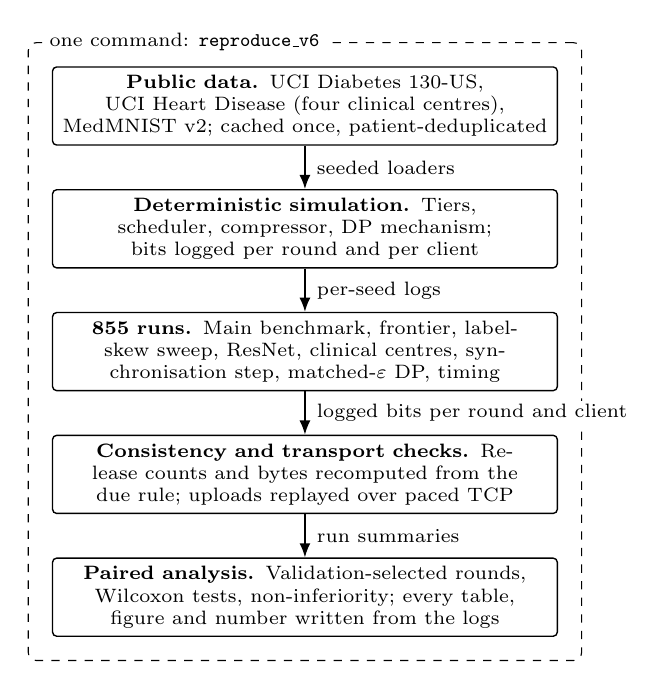
\begin{tikzpicture}[node distance=5.5mm, every node/.style={font=\scriptsize}]
\node[proc, text width=62mm] (d) {\textbf{Public data.} UCI Diabetes 130-US, UCI Heart Disease (four clinical centres), \mbox{MedMNIST v2}; cached once, patient-deduplicated};
\node[proc, text width=62mm, below=of d] (s) {\textbf{Deterministic simulation.} Tiers, scheduler, compressor, DP mechanism; bits logged per round and per client};
\node[proc, text width=62mm, below=of s] (r) {\textbf{\num{tmRuns} runs.} Main benchmark, frontier, label-skew sweep, ResNet, clinical centres, synchronisation step, matched-$\varepsilon$ DP, timing};
\node[proc, text width=62mm, below=of r] (e) {\textbf{Consistency and transport checks.} Release counts and bytes recomputed from the due rule; uploads replayed over paced TCP};
\node[proc, text width=62mm, below=of e] (a) {\textbf{Paired analysis.} Validation-selected rounds, Wilcoxon tests, non-inferiority; every table, figure and number written from the logs};
\draw[arr] (d) -- node[lab, right=1mm] {seeded loaders} (s);
\draw[arr] (s) -- node[lab, right=1mm] {per-seed logs} (r);
\draw[arr] (r) -- node[lab, right=1mm] {logged bits per round and client} (e);
\draw[arr] (e) -- node[lab, right=1mm] {run summaries} (a);
\begin{scope}[on background layer]
\node[grp, fit=(d)(s)(r)(e)(a), inner sep=3mm, label={[font=\scriptsize, fill=white, inner sep=2pt, anchor=west, xshift=2mm]north west:one command: \texttt{reproduce\_v6}}] {};
\end{scope}
\end{tikzpicture}
\caption{Pipeline of the study, from the public data to the reported numbers. All stages are run by one command, which first checks that repeated runs are bit-identical.}
\label{fig:pipeline}
\end{figure}

\subsection{Metrics}
\label{sec:metrics}
The patients of each client are split into training, validation and test sets (70/10/20\%, patient-grouped), and $\mathcal V_k$ and $\mathcal T_k$ denote the last two. With $\mathrm{AUC}_k^{\mathcal T}(r)$ the AUROC of client $k$'s own model after round $r$ on $\mathcal T_k$, the personalised AUROC and the reported round are
\begin{equation}
\begin{gathered}
A^{\mathcal T}(r)=\frac{\sum_{k}|\mathcal T_k|\,\mathrm{AUC}^{\mathcal T}_k(r)}{\sum_{k}|\mathcal T_k|},\\
\hat r=\min\Big\{\arg\max_{r\le R}A^{\mathcal V}(r)\Big\},
\end{gathered}
\label{eq:metric}
\end{equation}
where $A^{\mathcal V}$ is the same average over the validation splits. Clients whose split contains a single class are left out of the corresponding average, identically for every method. The primary metric is $A^{\mathcal T}(\hat r)$, and test data are never used to select anything.

The cost paired with it is the upload. With $b_{k,t}$ the bits that client $k$ sends in round $t$, the cumulative upload after round $r$ is
\begin{equation}
B(r)=\frac{1}{8\cdot10^{6}}\sum_{t=1}^{r}\sum_{k}b_{k,t}\quad\text{(MB)}.
\label{eq:upload}
\end{equation}
Two readings of (\ref{eq:upload}) are reported and are kept apart throughout. $B(\hat r)$ is the upload needed to obtain the reported model and is the cost that belongs to the primary metric. $B(R)$ is the upload of the whole training budget of $R=60$ rounds, which a deployment without early stopping would send. A full-rate method continues to transmit after its selected round, so $B(R)$ shows a larger saving for sparse schedules than $B(\hat r)$ does, and every statement about a saving names the reading on which it is based.

Secondary metrics are the mean of $A^{\mathcal T}$ over the last ten rounds, over the rounds of the last twenty that directly follow a synchronisation, and at $r=R$; the expected calibration error (ECE) and the Brier score~\cite{vancalster2019} before and after Platt scaling~\cite{platt1999} fitted on $\mathcal V_k$; and the AUROC of the worst client, $\min_k\mathrm{AUC}^{\mathcal T}_k(\hat r)$. Fig.~\ref{fig:pipeline} summarises the study.

\subsection{Problem Statement}
Given a quota $\rho$ on the payload fraction (\ref{eq:payload}), optionally a cap $\pi$ on the payload of any single round and a privacy budget $(\varepsilon^\star,\delta)$, the scheduler chooses intervals $\mathbf K$ and phases $\boldsymbol\phi$ for
\begin{equation}
\max_{\mathbf K,\boldsymbol\phi}\ A^{\mathcal T}(\hat r)\quad\text{s.t.}\quad\Pi_\infty(\mathbf K)\le\rho,\quad\hat P\le\pi,\quad\varepsilon(\mathbf K)\le\varepsilon^\star .
\label{eq:problem}
\end{equation}
A schedule is regarded as successful if $A^{\mathcal T}(\hat r)$ is non-inferior to that of full-rate personalisation and at least as high as that of the best uniform period at the same bytes. The objective is not known before training, so Section~\ref{sec:method} optimises a surrogate. The quantity $\varepsilon(\mathbf K)$ is defined only for a schedule that is fixed before training, because the accountant charges only data-independent releases.

\section{Quota-Constrained Multi-Rate Scheduling}
\label{sec:method}

The scheduler separates four decisions: which parameters are sent (the tiers), when they are sent (per-tier intervals chosen under the quota), how large an upload is (an optional compressor), and how private it is (the DP mechanism and its accountant). Fig.~\ref{fig:arch} shows the architecture.

\begin{figure*}[t]
\centering
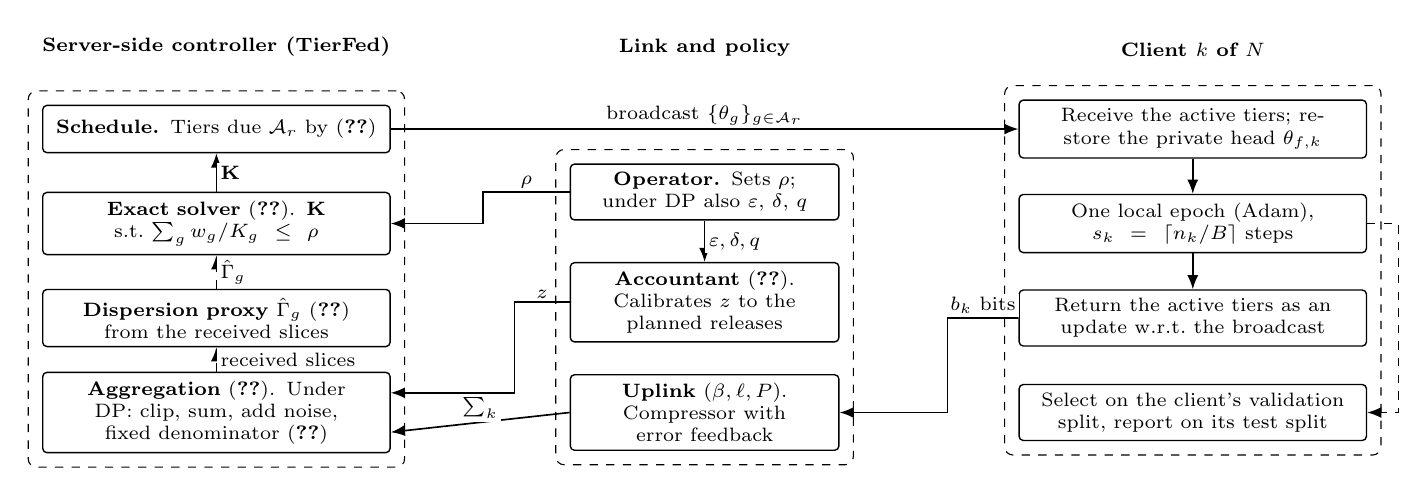
\begin{tikzpicture}[x=1mm,y=1mm]
\node[hdr] at (0,8) {Server-side controller (\tierfed{})};
\node[hdr] at (62,8) {Link and policy};
\node[hdr] at (124,8) {Client $k$ of $N$};
% server column
\node[srvbox, text width=42mm] (sched) at (0,0)   {\textbf{Schedule.} Tiers due $\mathcal A_r$ by (\ref{eq:due})};
\node[srvbox, text width=42mm] (solve) at (0,-12) {\textbf{Exact solver} (\ref{eq:ip}). $\mathbf K$ s.t.\ $\sum_g w_g/K_g\le\rho$};
\node[srvbox, text width=42mm] (disp)  at (0,-24) {\textbf{Dispersion proxy} $\Gh_g$ (\ref{eq:gammahat}) from the received slices};
\node[srvbox, text width=42mm] (agg)   at (0,-36) {\textbf{Aggregation} (\ref{eq:agg}). Under DP: clip, sum, add noise, fixed denominator (\ref{eq:dp})};
% link column
\node[lnkbox, text width=32mm] (op)   at (62,-8)  {\textbf{Operator.} Sets $\rho$; under DP also $\varepsilon$, $\delta$, $q$};
\node[lnkbox, text width=32mm] (acc)  at (62,-22) {\textbf{Accountant} (\ref{eq:rdp}). Calibrates $z$ to the planned releases};
\node[lnkbox, text width=32mm] (link) at (62,-36) {\textbf{Uplink} $(\beta,\ell,P)$. Compressor with error feedback};
% client column
\node[stebox, text width=42mm] (bcast) at (124,0)   {Receive the active tiers; restore the private head $\theta_{f,k}$};
\node[stebox, text width=42mm] (train) at (124,-12) {One local epoch (Adam), $s_k=\lceil n_k/B\rceil$ steps};
\node[stebox, text width=42mm] (ret)   at (124,-24) {Return the active tiers as an update w.r.t.\ the broadcast};
\node[stebox, text width=42mm] (eval)  at (124,-36) {Select on the client's validation split, report on its test split};
\begin{scope}[on background layer]
\node[grp, fit=(sched)(solve)(disp)(agg)] {};
\node[grp, fit=(op)(acc)(link)] {};
\node[grp, fit=(bcast)(train)(ret)(eval)] {};
\end{scope}
% data path down the round (solid)
\draw[arr] (sched.east) -- node[lab, above] {broadcast $\{\theta_g\}_{g\in\mathcal A_r}$} (bcast.west);
\draw[arr] (bcast.south) -- (train.north);
\draw[arr] (train.south) -- (ret.north);
\draw[arr] (ret.west) -- ++(-9,0) node[lab, above, pos=0.5] {$b_k$ bits} |- (link.east);
\draw[arr] (link.west) -- node[lab, above] {$\sum_k$} ([yshift=-2.5mm]agg.east);
% policy inputs (solid)
\draw[arr] (op.west) -- ++(-11,0) node[lab, above, pos=0.5] {$\rho$} |- (solve.east);
\draw[arr] (op.south) -- node[lab, right] {$\varepsilon,\delta,q$} (acc.north);
\draw[arr] (acc.west) -- ++(-7,0) node[lab, above, pos=0.5] {$z$} |- ([yshift=2.5mm]agg.east);
% measurements fed back (dashed)
\draw[meas] (agg.north) -- node[lab, right] {received slices} (disp.south);
\draw[meas] (disp.north) -- node[lab, right] {$\Gh_g$} (solve.south);
\draw[arr]  (solve.north) -- node[lab, right] {$\mathbf K$} (sched.south);
\draw[meas] (train.east) -- ++(4,0) |- (eval.east);
\end{tikzpicture}
\caption{Architecture of the scheduler and its environment. Solid arrows carry data and policy inputs, and dashed arrows carry measurements that are fed back. Only the active tiers are broadcast and replaced at the client (\ref{eq:restart}); the other tiers stay at the client and continue to be trained. Under DP the dashed path from the received slices to the solver is removed, and the schedule is planned before training (Section~\ref{sec:method-privacy}).}
\label{fig:arch}
\end{figure*}

\subsection{Dispersion Measurement}
\label{sec:dispersion}
\tierfed{} estimates how strongly the clients disagree on each tier from the slices that it receives. For tier $g$ with tensors $j\in g$,
\begin{equation}
\Gh_g^{(r)}=\frac{\sum_{j\in g}\frac1{|\mathcal S_r|}\sum_{k\in\mathcal S_r}\big\|\theta_{k,j}^{(r,s_k)}-\bar\theta_j^{(r)}\big\|_2^2}{\sum_{j\in g}\big\|\bar\theta_j^{(r)}\big\|_2^2+\xi_0},
\label{eq:gammahat}
\end{equation}
where $\bar\theta_j^{(r)}$ is the unweighted mean of the received tensors and $\xi_0=10^{-12}$. The ratio is scale-free, which makes tiers of different magnitude comparable. It is available only for the tiers received in round $r$, and the last value is carried forward for the others.

Under the restart step the received slices are one local epoch away from a common value, so $\Gh_g$ does not depend on the interval that preceded the upload, and the controller does not measure the effect of its own earlier decisions. The logs confirm this. For uniform periods $K$ from 1 to 8 on the main benchmark, the mean of $\Gh_g$ over the synchronisation rounds after warm-up lies between \num{tmDispRsSlowMin} and \num{tmDispRsSlowMax} ($\times10^{-3}$) for the slow tier and between \num{tmDispRsMedMin} and \num{tmDispRsMedMax} for the medium tier (supplement, Table~\sref{tab:dispersion}). Under the carry-over step the same quantity grows with the interval, by factors of \num{tmDispRatioSlowFour} and \num{tmDispRatioMedFour} for the two tiers at $K=4$ and of \num{tmDispRatioSlowEight} and \num{tmDispRatioMedEight} at $K=8$.

\subsection{Cost of an Interval, Programme and Closed Form}
\label{sec:programme}
\emph{Assumptions.} The analysis concerns the shared tiers with the private heads held fixed, local SGD with step size $\eta$ in place of Adam, the same number $s$ of local steps at every client, and equal aggregation weights $1/N$. Each $F_k$ is assumed to be block separable, $F_k(\theta)=\sum_gF_{k,g}(\theta_g)$, with $L$-smooth blocks, so that the gradient of a tier does not depend on the other tiers; this removes the coupling between tiers and is the main idealisation. Stochastic gradients are unbiased with variance at most $\sigma_g^2$ on tier $g$, the heterogeneity of tier $g$ is bounded, $\frac1N\sum_k\|\nabla_gF_k(\theta)-\nabla_gF(\theta)\|^2\le\Gamma_g$, and $F_g=\frac1N\sum_kF_{k,g}$ is bounded below by $F_g^\star$~\cite{stich2019,wang2021coop}. The experiments depart from these assumptions in that they use Adam, $s_k=\lceil n_k/B\rceil$ steps, sample weights and a coupled network, and with unequal $s_k$ plain averaging converges towards a reweighted objective~\cite{wang2020fednova}. The two propositions describe the idealised system. They motivate the schedule and are not used to predict accuracy.

\begin{proposition}[Cost of an interval under the restart step]
\label{prop:bound}
Let tier $g$ be synchronised every $K_g$ rounds by (\ref{eq:restart})--(\ref{eq:adopt}). There are absolute constants $c_0,c_1,c_2$ such that the following holds for $\eta\le c_0/(LK_{\max}s)$.

\noindent(a) \emph{Client copies.} After $m\ge1$ local epochs from a common value of tier $g$, with $\bar\theta_g=\frac1N\sum_k\theta_{k,g}$,
\begin{equation}
\frac1N\sum_{k=1}^N\mathbb E\big\|\theta_{k,g}-\bar\theta_g\big\|^2\le c_2\,\eta^2s^2m^2\big(\Gamma_g+\sigma_g^2\big),
\label{eq:drift}
\end{equation}
and $m\le\max(1,K_g-1)\le K_g$ at every point of the schedule.

\noindent(b) \emph{Server copy.} Let $r_1<\dots<r_{J_g}$ be the rounds up to $R$ in which tier $g$ is due, and $D_g=F_g(\theta_g^{(1)})-F_g^\star$. Then
\begin{align}
\min_{1\le j\le J_g}\mathbb E\big\|\nabla_gF(\theta^{(r_j)})\big\|^2
&\le \frac{c_1D_g}{\eta sJ_g}+c_1\eta L\,\frac{\sigma_g^2}{N}\notag\\
&\quad+c_2\,\eta^2L^2s^2\big(\Gamma_g+\sigma_g^2\big).
\label{eq:bound}
\end{align}
\end{proposition}
The proof is given in the supplement (Section~\sref{supp:proofs}). Part (a) is the drift lemma of local SGD~\cite{stich2019,khaled2020} applied to one tier. Part (b) holds because, under block separability, the steps that a client takes on a tier between two synchronisations of that tier never enter the server copy, so the synchronisations of tier $g$ form a sequence of $J_g$ rounds of federated averaging with $s$ local steps~\cite{wang2020fednova,karimireddy2020}. The variance in the second term of (\ref{eq:bound}) is divided by $N$ because every step of the averaged model combines one stochastic gradient from each client. These $N$ gradients are independent, each has a variance of at most $\sigma_g^2$, and their average with equal weights therefore has a variance of at most $\sigma_g^2/N$, which is the linear speed-up of local SGD in the number of clients. With the sample weights $p_k$ of (\ref{eq:agg}) the factor $1/N$ becomes $\sum_kp_k^2=1/N_{\mathrm{eff}}$. On the main benchmark $\sum_kp_k^2=\num{tmSumPSq}$, which corresponds to $N_{\mathrm{eff}}=\num{tmNeff}$ for $N=20$, and at the clinical centres $N_{\mathrm{eff}}=\num{tmHospNeff}$ for $N=4$.

Under the restart step an interval therefore has two costs. By (\ref{eq:bound}), the server copy of tier $g$ receives $J_g\approx T_w+(R-T_w)/K_g$ aggregation rounds instead of $R$, so the first term grows in proportion to $K_g$ while the last term does not depend on $K_g$. By (\ref{eq:drift}), the clients' own copies, which are the models that are evaluated, drift apart between synchronisations by an amount that grows as $K_g^2$. Under the carry-over step the two costs merge into the bound of local SGD with period $K_gs$~\cite{wang2021coop}: the $K_g$ local epochs enter the average, $J_g$ is replaced by $R$, and the last term of (\ref{eq:bound}) becomes $c_2\eta^2L^2s^2K_g^2(\Gamma_g+\sigma_g^2)$. In both cases $K_g^2(\Gamma_g+\sigma_g^2)$ measures what a long interval costs on tier $g$, and it is small only for a tier on which the clients agree.

\emph{Programme.} Given a quota $\rho$, the controller solves
\begin{equation}
\mathbf K^\star=\arg\min_{K_g\in\{1,\dots,K_{\max}\}}\sum_{g\in\mathcal G_{\mathrm{sh}}}K_g^2\,\Gh_g\ \ \text{s.t.}\ \sum_{g\in\mathcal G_{\mathrm{sh}}}\frac{w_g}{K_g}\le\rho .
\label{eq:ip}
\end{equation}
The objective is the right-hand side of (\ref{eq:drift}) at its largest value $m=K_g$, summed over the shared tiers, with the measured $\Gh_g$ in the place of $\Gamma_g+\sigma_g^2$; the factor $c_2\eta^2s^2$ is common to the tiers and does not change the minimiser. The proxy is not an estimate of $\Gamma_g+\sigma_g^2$. Its numerator is the dispersion after one local epoch, in which the noise and the heterogeneity enter with different powers of $s$, and its denominator is the squared norm of the tier, which differs between tiers. The programme does not contain the server-side cost of (\ref{eq:bound}) either. The programme is thus a heuristic surrogate, and every statement below about (\ref{eq:ip}) concerns this surrogate. With the head private, $\mathcal G_{\mathrm{sh}}=\{\mathrm s,\mathrm m\}$ and $K_{\max}=8$, the programme has 64 candidates and is solved by enumeration, with ties broken in favour of the denser schedule.

\begin{proposition}[Closed form and the value of differentiation]
\label{prop:cuberoot}
Let $\Gamma_g>0$, $w_g>0$, $\sum_gw_g=1$, and relax $K_g$ to the positive reals. Then (\ref{eq:ip}) has the unique minimiser
\begin{equation}
K_g^\star=\Big(\frac{w_g}{\Gamma_g}\Big)^{1/3}\frac{S}{\rho},\qquad S=\sum_hw_h^{2/3}\Gamma_h^{1/3},
\label{eq:cuberoot}
\end{equation}
with value $J^\star=S^3/\rho^2$. The uniform interval $K=1/\rho$ costs $J_{\mathrm u}=\sum_g\Gamma_g/\rho^2$, and
\begin{equation}
\Psi=1-\frac{J^\star}{J_{\mathrm u}}=1-\frac{S^3}{\sum_g\Gamma_g}\in[0,1),
\label{eq:psi}
\end{equation}
with $\Psi=0$ if and only if $w_g/\Gamma_g$ is the same for all tiers. When $1/\rho$ is an integer, no integer schedule lowers the objective of (\ref{eq:ip}) below that of the uniform period by more than the fraction $\Psi$.
\end{proposition}
The proof (supplement, Section~\sref{supp:proofs}) uses the KKT conditions of the convex programme, H\"older's inequality with exponents $3/2$ and $3$ for $\Psi\ge0$, and the integer feasibility of $K=1/\rho$. Two properties of the closed form are used in the evaluation. First, the ratio of two intervals, $K_a/K_b=(w_a\Gamma_b/w_b\Gamma_a)^{1/3}$, compresses differences between tiers: a factor of eight in the ratio of payload to dispersion is needed for a factor of two in the interval, so tiers with similar ratios receive the same interval after rounding. Second, the proposition holds for any positive weights and therefore applies exactly to (\ref{eq:ip}) with $\Gh_g$ in the place of $\Gamma_g$. $\Psi$ is invariant to a factor common to all tiers. Evaluated on $\Gh_g$ at the end of warm-up, it states, before any sparse round has taken place, by how much a per-tier schedule can lower the surrogate below a uniform one. It does not state how much accuracy such a reduction is worth.

\subsection{Schedule Rule, Phases and the Quota}
Rounds are indexed $r=1,\dots,R$. The first $T_w$ rounds synchronise every shared tier, and thereafter tier $g$ is due when
\begin{equation}
\mathcal A_r=\begin{cases}\mathcal G_{\mathrm{sh}}, & r\le T_w,\\ \{g:\ (r-T_w-\phi_g)\bmod K_g=0\}, & r>T_w,\end{cases}
\label{eq:due}
\end{equation}
with phase $\phi_g=0$ unless the tiers are staggered. The fixed periods, the DP planner and the accountant all use this rule, and the consistency check of Section~\ref{sec:results-check} recomputes every release from it. Adaptive \tierfed{} sends tier $g$ when at least $K_g$ rounds have passed since its last synchronisation, which coincides with (\ref{eq:due}) whenever $\mathbf K$ is constant after warm-up. $T_w=5$ and $K_{\max}=8$ throughout. Fig.~\ref{fig:round} shows one round at the server.

\emph{Phases and the peak.} A quota on the mean does not bound the payload $P_r$ of a single round, because tiers with aligned phases are due together and then send the full shared payload. Two tiers with phases $\phi_a$ and $\phi_b$ are never due in the same round if and only if $\phi_a-\phi_b\not\equiv0\pmod{\gcd(K_a,K_b)}$ (supplement, Section~\sref{supp:proofs}). With $\gcd(K_a,K_b)\ge2$ the offset $\lfloor\gcd/2\rfloor$ separates them and bounds the peak after warm-up by $\max_gw_g$ at the same long-run payload fraction $\Pi_\infty$; over a finite horizon $\Pi_R$ can differ slightly, because the phase changes which synchronisations fall inside it. With co-prime intervals no phase separates the tiers. The staggered variant adds the constraint $\max_{r>T_w}P_r\le\pi$ to (\ref{eq:ip}) and checks it over one hyper-period $\mathrm{lcm}(\mathbf K)$. The warm-up rounds still send the whole payload, and they can be sent with eight-bit quantisation to lower their peak as well.

\emph{The quota.} Solving (\ref{eq:ip}) with $\rho$ bounds $\Pi_\infty$ of (\ref{eq:payload}) and not the realised $\Pi_R$: a warm-up of $T_w$ rounds at payload fraction $c_w$ adds $T_w(c_w-\Pi_\infty)/R$ to the realised fraction. A quota over all rounds is met by solving with $\rho'=(\rho R-c_wT_w)/(R-T_w)$. Both forms are reported, and the realised $\Pi_R$ is read from the logs.

\begin{figure}[t]
\centering
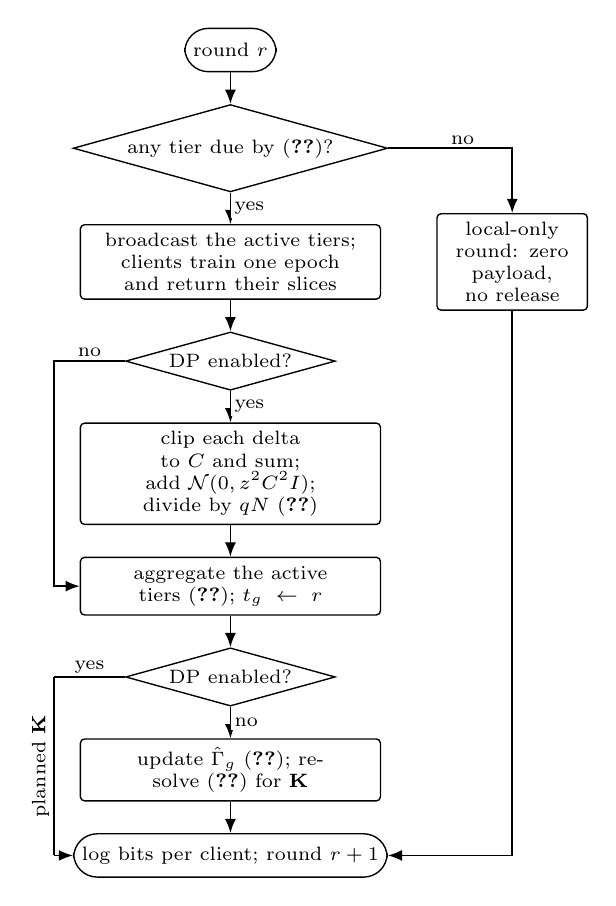
\begin{tikzpicture}[node distance=4mm and 6mm, every node/.style={font=\scriptsize}]
\node[term] (start) {round $r$};
\node[dec, below=of start] (due) {any tier due by (\ref{eq:due})?};
\node[proc, text width=36mm, below=of due] (bc) {broadcast the active tiers; clients train one epoch and return their slices};
\node[dec, below=of bc] (dp) {DP enabled?};
\node[proc, text width=36mm, below=of dp] (priv) {clip each delta to $C$ and sum;\\ add $\mathcal N(0,z^2C^2I)$;\\ divide by $qN$ (\ref{eq:dp})};
\node[proc, text width=36mm, below=of priv] (ag) {aggregate the active tiers (\ref{eq:agg}); $t_g\leftarrow r$};
\node[dec, below=of ag] (dp2) {DP enabled?};
\node[proc, text width=36mm, below=of dp2] (upd) {update $\Gh_g$ (\ref{eq:gammahat}); re-solve (\ref{eq:ip}) for $\mathbf K$};
\node[term, below=of upd] (next) {log bits per client; round $r+1$};
\node[proc, text width=17mm, right=7mm of bc] (local) {local-only round: zero payload, no release};
\draw[arr] (start) -- (due);
\draw[arr] (due) -- node[lab, right] {yes} (bc);
\draw[arr] (due.east) -| node[lab, above, pos=0.3] {no} (local);
\draw[arr] (local.south) |- (next.east);
\draw[arr] (bc) -- (dp);
\draw[arr] (dp) -- node[lab, right] {yes} (priv);
\draw[arr] (dp.west) -- ++(-9mm,0) node[lab, above, pos=0.5] {no} |- (ag.west);
\draw[arr] (priv) -- (ag);
\draw[arr] (ag) -- (dp2);
\draw[arr] (dp2) -- node[lab, right] {no} (upd);
\coordinate (k1) at ($(dp2.west)+(-9mm,0)$);
\coordinate (k2) at (k1 |- next.west);
\draw[line width=0.6pt] (dp2.west) -- node[lab, above] {yes} (k1);
\draw[line width=0.6pt] (k1) -- node[midway, rotate=90, anchor=south, font=\scriptsize, inner sep=1.5pt] {planned $\mathbf K$} (k2);
\draw[arr] (k2) -- (next.west);
\draw[arr] (upd) -- (next);
\end{tikzpicture}
\caption{Flow of one round at the server. In a local-only round the clients still train their own copies. Under DP the schedule is fixed before training, and the dispersion is never computed from the private slices.}
\label{fig:round}
\end{figure}

\emph{Compression.} An optional compressor acts on each client's update relative to the broadcast, with error feedback. It emits a fraction $\kappa\in(0,1]$ of the float32 bits, and the bits that it emits are the bits that are counted.

\subsection{Privacy: Threat Model, Mechanism and Eligible Schedules}
\label{sec:method-privacy}
\emph{Threat model.} Clients send their updates over TLS to an aggregator that is trusted to apply the mechanism and sees the raw updates, as in central DP-FedAvg~\cite{mcmahan2018dp}. Central DP protects the released aggregates against those who receive them, the other clients among them. A passive network observer cannot read the payloads but sees when each client transmits and how many bytes it sends, which is exactly the schedule. A schedule that depends on client data can leak for this reason even when every payload is encrypted. Secure aggregation with distributed noise~\cite{kairouz2021ddg} would remove the trust in the aggregator but not this metadata. Poisoning is outside the scope of this article.

\emph{Mechanism.} In each round every client joins the cohort $\mathcal S_r$ independently with probability $q$. Full participation, $q=1$, is the primary cross-silo setting, and $q<1$ is examined as a sensitivity analysis. The server clips the update $\Delta_k=\theta_k^{(r,s_k)}-\theta^{(r)}$ of every participating client on the due tiers and adds noise to the sum before dividing by the \emph{fixed} expected cohort size,
\begin{equation}
\tilde\Delta=\frac1{qN}\Big(\sum_{k\in\mathcal S_r}\Delta_k\min\big(1,\tfrac{C}{\|\Delta_k\|_2}\big)+\mathcal N(0,z^2C^2I)\Big),
\label{eq:dp}
\end{equation}
which is the fixed-denominator estimator of DP-FedAvg~\cite{mcmahan2018dp}. Adding or removing one client changes the sum by at most $C$ in $\ell_2$ norm, and the denominator reveals nothing about the realised cohort; a planned release whose cohort is empty still adds noise. Because of the restart step, $\Delta_k$ is the result of one local epoch for every schedule, so the clipping norm $C$ has the same meaning for all of them. The server applies the mechanism to every method in the same way.

\emph{Accountant.} Over the $R_{\mathrm{tx}}$ planned releases, the R\'enyi DP of the Poisson-subsampled Gaussian mechanism is composed at integer orders~\cite{mironov2019sgm},
\begin{align}
\varepsilon_\alpha&=\frac{R_{\mathrm{tx}}}{\alpha-1}\log\sum_{k=0}^{\alpha}\binom{\alpha}{k}(1-q)^{\alpha-k}q^ke^{\frac{k^2-k}{2z^2}},\notag\\
\varepsilon&=\min_\alpha\Big\{\varepsilon_\alpha+\frac{\log(1/\delta)}{\alpha-1}\Big\},
\label{eq:rdp}
\end{align}
with $\delta=10^{-5}$; for $q=1$ this reduces to $R_{\mathrm{tx}}\alpha/(2z^2)$~\cite{mironov2017}. The implementation is checked against the TensorFlow-Privacy reference and the closed form for $q=1$ (supplement, Section~\sref{supp:dp}). At $q=1$ the exact privacy of $R_{\mathrm{tx}}$ Gaussian releases is $\mu$-Gaussian DP with $\mu=\sqrt{R_{\mathrm{tx}}}/z$~\cite{dong2022gdp,balle2018}. This exact accountant and (\ref{eq:rdp}) both depend on $R_{\mathrm{tx}}$ only through $R_{\mathrm{tx}}/z^2$, so the exact one would lower the noise multiplier of every method by the same factor, between \num{gdpSigmaCutEightPct}\% and \num{gdpSigmaCutOnePct}\% for $\varepsilon^\star$ from 8 to 1 (supplement, Section~\sref{supp:dp}). The comparison at matched $\varepsilon$ is unaffected by the choice of accountant, and every reported $\varepsilon$ is an upper bound. The multiplier $z$ is calibrated to the release count of each method by bisection on (\ref{eq:rdp}).

\emph{Which schedules are covered.} The accountant covers a release only if the decision to release does not depend on the private data. This holds for FedAvg, FedProx, FedPer, local training, a fixed period and the planner described below, whose release rounds are fixed before training. It does not hold for adaptive \tierfed{}, AdaComm, LAG or the FedLAMA-style rule, whose schedules are functions of client updates or losses, and the released code refuses to run these under DP. Privacy filters and odometers~\cite{rogers2016odometer} and the sparse vector technique~\cite{lyu2017svt} charge for data-dependent release decisions, whereas FL schedulers take such decisions without charging for them. DP-FTRL~\cite{kairouz2021ftrl} and matrix-factorisation mechanisms~\cite{choquette2023banded} are suited to full participation but also require data-independent release rounds, and they are not evaluated here.

\emph{Planning under a privacy budget (\tierfed{}-DP).} A planner that respects the accountant chooses $\mathbf K$ before training from public quantities only: $(\varepsilon^\star,\delta)$, $q$, $R$, $T_w$, $w_g$ and $\rho$. For each candidate it computes the release set of (\ref{eq:due}) and the smallest $z(\mathbf K)$ that keeps these releases $(\varepsilon^\star,\delta)$-DP, and it minimises
\begin{equation}
J(\mathbf K)=\frac{\sum_g w_gK_g^2}{K_{\max}^2}+\lambda\,\frac{\sum_{r}P_r(\mathbf K)\,z(\mathbf K)^2}{\sum_{r}P_r(\mathbf 1)\,z(\mathbf 1)^2}
\label{eq:jdp}
\end{equation}
over the candidates whose realised payload fraction $\Pi_R$, warm-up included, is within the quota. The first term is the drift cost of (\ref{eq:ip}) under a flat prior $\Gamma_g\propto w_g$, the second is the injected noise energy, and each is normalised by its largest value; fewer releases need less noise but allow more drift. Under the flat prior Proposition~\ref{prop:cuberoot} gives $\Psi=0$, so the relaxed minimiser of the first term is a uniform period. The integer planner is not restricted to equal intervals, however. Evaluated on a grid of \num{tmPlanCells} combinations of the prior weight $\lambda$ and the quota (supplement, Table~\sref{tab:planner}), it returns equal intervals in \num{tmPlanCellsEqual} of them, among which are all those in which the quota does not bind\claim{tmPlanEqualWithoutQuota}, and the unequal pair \num{tmPlanUnequalPairs} in the remaining \num{tmPlanCellsUnequal}, all at $\rho=\num{tmPlanUnequalRho}$, where the warm-up rounds make $(4,4)$ infeasible; the choice does not depend on $\varepsilon^\star$\claim{tmPlanEpsFree}. In the DP experiments of this article, which use $\rho=1$ and $\lambda=1$, the planner selects $\num{tmDpPlannerK}$ in every seed\claim{tmDpPlannerSameK}. It is evaluated as an ablation of planning under a budget and is not claimed as a contribution.

\section{Experimental Setup}
\label{sec:setup}
Every method is run under the protocol of Section~\ref{sec:system} on the same seeds and data splits, and every number is read from the logs. This section lists the experiment families, the baselines and reference bounds, the privacy and timing experiments, and the statistical procedure that decides each comparison.


\textbf{Experiment families.} The main protocol comprises \num{tmRuns} runs, which are listed by family in the supplement (Table~\sref{tab:families}): the main comparison on the specialty groups and at the clinical centres, the accuracy--upload frontier with the communication parameter of every method swept, the label-skew sweep and the ResNet backbone, which examine the regimes to which Proposition~\ref{prop:cuberoot} points, the round-sparse schedules with the carry-over step of Section~\ref{sec:federation}, and the matched-$\varepsilon$, timing and peak-aware runs. Additional experiments that were read at the final round without a validation split are reported in Section~\sref{supp:legacy} of the supplement and are identified there as such.

\textbf{Baselines and bounds.} The full-rate methods are FedAvg~\cite{mcmahan2017}, FedProx~\cite{li2020fedprox} and FedPer~\cite{arivazhagan2019}, the last of which is the reference of the non-inferiority tests. The round-sparse methods are AdaComm~\cite{wang2019adacomm}, LAG~\cite{chen2018lag}, a FedLAMA-style per-layer interval rule reimplemented from its published description~\cite{lee2023fedlama}, and fixed periods on (\ref{eq:due}) with the private head and the warm-up of \tierfed{}. LAG is run with the sample weights of (\ref{eq:agg}) and, as a variant, with equal client weights. All round-sparse methods run on the protocol of Section~\ref{sec:federation}, restart step included, so that the comparison isolates the schedule; AdaComm and the fixed local period as published upload the result of all local steps since the last synchronisation, which corresponds to the carry-over step of Section~\ref{sec:results-sync}. Three references bound the task: local training without communication, a centralised MLP trained on the pooled training splits of all clients for the same number of passes, and gradient boosting~\cite{ke2017lightgbm}. All three are scored on the same per-client test splits, with the round, epoch or iteration chosen on validation. SCAFFOLD~\cite{karimireddy2020}, whose control variates are defined for SGD, is reported with an SGD local solver in the supplement.

\textbf{Differential privacy.} FedPer, the fixed periods $K=4$ and $K=8$, one-shot federation (no warm-up and a single release in round $R$, after a data-independent broadcast of the initial model) and the planner are run at $\varepsilon^\star=4$, $\delta=10^{-5}$, $q=1$ and $C=1$, each with $z$ calibrated to its own release count. Local training is the reference with $\varepsilon=0$ on the same splits. Sweeps with $q<1$ over $\varepsilon^\star\in\{1,2,4,8\}$ for 20 and 100 clients are reported in the supplement.

\textbf{Timing side channel.} One target client holds half of its labels flipped (shifted world) or none (clean world). A passive observer sees which rounds carry traffic and how many bytes each client sends, and summarises a run by one of four observables $o$: the number of rounds with traffic, the number of rounds in which the target transmits, the bytes of the target, or the bytes of all clients. The power of the observer is the Mann--Whitney AUC over the $n_1$ shifted and $n_0$ clean runs,
\begin{equation}
\mathrm{AUC}=\frac1{n_1n_0}\sum_{i=1}^{n_1}\sum_{j=1}^{n_0}\Big(\mathbb 1\big[o^{(1)}_i>o^{(0)}_j\big]+\tfrac12\,\mathbb 1\big[o^{(1)}_i=o^{(0)}_j\big]\Big),
\label{eq:auc}
\end{equation}
which equals 0.5 when the schedule reveals nothing. Its significance is assessed by a permutation test: the statistic is the largest value of $|\mathrm{AUC}-0.5|$ over the four observables, and its null distribution is obtained from 10,000 random reassignments of the runs to the two worlds, which accounts for the choice among observables. A schedule is reported as leaking when $|\mathrm{AUC}-0.5|\ge0.25$ on at least one observable and the permutation $p$-value is below 0.05.

\textbf{Statistics.} All comparisons are paired across seeds. Two primary contrasts were fixed in the code before the runs, together with the metric and both thresholds: \tierfed{} against FedPer, and \tierfed{} against the best uniform period at matched bytes. With $\mathcal U$ the uniform periods run in a setting, $B_K$ the mean upload $B(R)$ of period $K$, $B_{\mathrm{TF}}$ that of \tierfed{} and $\bar A^{\mathcal V}_K$ the mean validation AUROC at $\hat r$, the best uniform period and the gain over it are
\begin{equation}
\begin{gathered}
K_{\mathrm u}=\arg\max_{K\in\mathcal U:\,B_K\le1.05\,B_{\mathrm{TF}}}\bar A^{\mathcal V}_K,\\
\Delta_{\mathrm u}=\frac1S\sum_{s=1}^{S}\big(A^{\mathcal T}_{\mathrm{TF},s}-A^{\mathcal T}_{K_{\mathrm u},s}\big),
\end{gathered}
\label{eq:gate}
\end{equation}
over the $S$ seeds that both share. Every other comparison is exploratory. Tests are two-sided Wilcoxon signed-rank tests, and intervals are percentile bootstrap intervals over seeds with 10,000 resamples. The second contrast was first specified with a Holm-corrected $p<0.05$, which the smallest families cannot reach by construction, so $\Delta_{\mathrm u}$ is judged by its interval instead: a setting counts as a gain only if the 95\% interval excludes zero and $\Delta_{\mathrm u}\ge0.005$ AUROC. No setting meets either rule\claim{tmGateNoWin}\claim{tmGateNoHolmWin}. A difference below 0.005 AUROC is not called relevant, whatever its $p$-value. Non-inferiority to FedPer is tested one-sided,
\begin{equation}
H_0:\ \mathbb E[d]\le-\Delta_{\mathrm{NI}},\qquad d=A^{\mathcal T}_{\text{method}}(\hat r)-A^{\mathcal T}_{\text{FedPer}}(\hat r),
\label{eq:ni}
\end{equation}
by the signed-rank test on $d+\Delta_{\mathrm{NI}}$ with $\Delta_{\mathrm{NI}}=0.01$ and, as a sensitivity margin, 0.005. Repeated runs are bit-identical on one machine. On a second machine every data-independent schedule sends the same bytes, but the AUROC of a single run can change by up to \num{xmachineAurocDiff} (Section~\ref{sec:results-check}), so every comparison is computed within one machine.

\section{Results}
\label{sec:results}

This section reports the checks of the protocol, the main comparison on both benchmarks, the settings in which a per-tier schedule could be expected to help, the effect of the synchronisation step, the cost on constrained links, and privacy. Unless stated otherwise, values are means over seeds on the readmission data with the MLP and the specialty groups, and $p$-values are from paired Wilcoxon tests.

\subsection{Protocol Checks}
\label{sec:results-check}
The consistency check recomputes, from the stated rules, the transmitting rounds of every data-independent schedule, the bits of every uncompressed round with full participation and the releases charged by the accountant, over all \num{consLogs} logs of this article. It finds \num{consFailed} mismatches in \num{consChecksSchedule} schedule checks, \num{consChecksBits} byte checks and \num{consChecksAccountant} accountant checks.

All runs of the main protocol were made on one Linux machine, and \num{xmachineRuns} of the label-skew and timing runs were repeated on a Windows laptop. Every data-independent schedule sends the same bytes in every round on both machines\claim{xmachineBytesIdentical}, and so do \num{xmachineAdaptiveSame} of the \num{xmachineAdaptivePairs} adaptive runs; the others differ by up to \num{xmachineAdaptiveMbPct}\%, because their decisions depend on floating-point values computed from client data. The AUROC at the selected round changes by a median of \num{xmachineAurocMedian} and by at most \num{xmachineAurocDiff}. The maximum occurs under strong label skew, where the validation curve is flat and a small numerical difference selects another round (\num{xmachineSelDiffer} runs). The outcome of the second primary contrast is the same on both machines, and for every schedule the observer AUC of the timing experiment lies on the same side of 0.75\claim{xmachineGateSame}\claim{xmachineTimingSame}.

Because the selected round can move in this way, both primary contrasts are repeated under two other rules: the first maximum of the trailing three-round mean of $A^{\mathcal V}$, and the mean of $A^{\mathcal T}$ over the last ten rounds, which involves no selection (supplement, Section~\sref{supp:selection}). Under none of the three rules is \tierfed{} ahead of the best uniform period by 0.005 AUROC with an interval above zero in any setting\claim{tmSelNoWin}. Its agreement with FedPer is less robust. Under the smoothed rule it is below FedPer by more than 0.005, with an interval below zero, in \num{tmSelSmoothBehindWord} of the \num{tmGateSettingsWord} settings (\num{tmSelSmoothBehindList}), because the first-maximum rule can select the peak that follows a synchronisation.

\begin{table*}[t]
\caption{Comparison of the Methods on the 20 Specialty Groups}
\label{tab:main}
\centering\footnotesize
\fit{\gen{tm_main}}
\tabnote{MLP, means over \num{tmMainSeeds} seeds. AUROC at $\hat r$: personalised test AUROC at the validation-selected round with its bootstrap 95\% interval. MB to $\hat r$ and MB, 60 rounds: the readings $B(\hat r)$ and $B(R)$ of the upload (\ref{eq:upload}). Last 10 and Phase: mean AUROC over the last ten rounds and over the post-synchronisation rounds of the last twenty. +FT~3: final model after three further local epochs. ECE: without and with Platt scaling. Worst group: lowest AUROC of a group at $\hat r$. $\Delta$ FedPer and $p$: paired difference from FedPer at $\hat r$ and its Wilcoxon $p$-value. The symbol $\equiv$ joins schedules that send the same tiers in every round and therefore produce identical runs.}
\end{table*}

\subsection{Main Comparison on the Specialty Groups}
\label{sec:results-main}
Table~\ref{tab:main} reports the main comparison. At the validation-selected round the federated methods are close to one another. FedPer reaches \num{auFedperAuroc}, and, with the exception of AdaComm, no method differs from it by more than \num{auFedSpread} AUROC, which is below the threshold of 0.005 that this study treats as relevant (the largest difference is that of \num{auFedSpreadName}, $p\num{auFedMinP}$). AdaComm differs from FedPer by \num{auAdacommEightDFedper} ($p\num{auAdacommEightDFedperP}$) with an upload of \num{tmAdacommMbSel}~MB up to its selected round, and local training differs by \num{auLocalDFedper} ($p\num{auLocalDFedperP}$), so federation improves on local training in this task.

\ifflag{auTierfedAlwaysFourFour}{\tierfed{} chooses $\mathbf K=(4,4)$ in every seed. After warm-up its schedule coincides with that of the fixed period $(4,4)$ in every round, the two runs are identical\claim{tmTierfedIsFixed}, and Table~\ref{tab:main} lists them in one row. This is the behaviour that Proposition~\ref{prop:cuberoot} predicts: $\Psi$ at the end of warm-up is \num{auGateSpecialtyPsi}\%, so no per-tier schedule can lower the surrogate by more than that fraction.}{\runreq} \tierfed{} is non-inferior to FedPer at $\Delta_{\mathrm{NI}}=0.01$ ($p\num{auTierfedNiTenP}$) and at 0.005 ($p\num{auTierfedNiFiveP}$); AdaComm is non-inferior at 0.01 ($p\num{auAdacommEightNiTenP}$) but not at 0.005 ($p\num{auAdacommEightNiFiveP}$).

The two readings of the upload give different savings, and they are stated separately. Up to the selected round \tierfed{} uploads \num{tmTierfedMbSel}~MB and FedPer \num{tmFedperMbSel}~MB, a saving of \num{tmSaveSelPct}\%. \tierfed{} selects round \num{tmTierfedRound} on average and FedPer round \num{tmFedperRound}, so this saving is obtained with about twice as many rounds. Over the 60 rounds the uploads are \num{tmTierfedMbAll} and \num{tmFedperMbAll}~MB, a saving of \num{tmSaveAllPct}\%, most of which comes from the rounds in which FedPer continues to transmit after its selected round (Fig.~\ref{fig:dyn}(b)).

\begin{figure*}[t]
\centering\fig{fig_dynamics}{\textwidth}
\caption{Training on the specialty groups (MLP, means over \num{tmMainSeeds} seeds). (a) Personalised test AUROC $A^{\mathcal T}(r)$ with its 95\% interval; the dot on each curve marks the mean selected round $\hat r$. The \tierfed{} curve is also that of Fixed $(4,4)$, and the LAG curve coincides with that of FedPer. (b) Cumulative upload $B(r)$ of all clients. (c) Upload of one client per round as a fraction of its shared payload, for the aligned and the staggered period $(4,4)$ (seed 42, rounds 1--21, of which rounds 1--5 are the warm-up).}
\label{fig:dyn}
\end{figure*}

The round at which a method is read has a large effect on the comparison. Full-rate training reaches its best validation round early, and its test AUROC then declines. Under a sparse schedule the test AUROC rises at each synchronisation and falls between synchronisations (Fig.~\ref{fig:dyn}(a)). Both effects follow from the restart step: the server copy advances by one aggregated epoch per synchronisation, so a period of four reaches a given state of the shared tiers about four times later, and the local epochs in between fit each client's copy to its own data. Over the last ten rounds the sparse schedules are consequently ahead (\tierfed{} \num{auTierfedLast}, FedPer \num{auFedperLast}), and a comparison at the final round would favour them, whereas at the validation-selected round the difference is \num{auTierfedDFedper}. Fine-tuning each client's final model for three further local epochs lowers the AUROC of every method, by \num{auFtLossMin} to \num{auFtLossMax}\claim{auFtAlwaysLowers}, which indicates that additional local adaptation does not account for the late-round difference. The two LAG rows of Table~\ref{tab:main} differ only in the aggregation weights. At its default threshold LAG never skips an upload; with sample weights its final-round AUROC is \num{auLagFinal}, level with FedAvg (\num{auFedavgFinal}), and with equal client weights it is \num{auLagUniformFinal}.

The AUPRC follows the same pattern (FedPer \num{auFedperAuprc}, \tierfed{} \num{auTierfedAuprc}, local training \num{auLocalAuprc}, against a prevalence of \num{diabetesmlpPrevalenceFrac}). Inverse-frequency class weighting shifts the scores of every method, so the raw ECE is between \num{auEceRawMin} and \num{auEceRawMax}; Platt scaling on each client's validation split lowers it to between \num{auEceCalMin} and \num{auEceCalMax} for every method at no communication cost. The AUROC of the worst group is between \num{auWorstMin} and \num{auWorstMax}, so the sample-weighted mean conceals groups for which no method is useful.


A direct paired comparison of \tierfed{} with each baseline is given in the supplement (Table~\sref{tab:paired}). \tierfed{} is above local training on \num{tmPairLocalHigher} seeds and above AdaComm on \num{tmPairAdacommEightHigher}; against every other federated method the difference is at most \num{tmPairRestMaxAbs} in absolute value, and no Holm-corrected test is significant\claim{tmPairRestNoneSig}.

\subsection{Comparison at the Four Clinical Centres}
\label{sec:results-centres}

\begin{table*}[t]
\caption{Comparison of the Methods at the Four Clinical Centres}
\label{tab:centres}
\centering\footnotesize
\fit{\gen{tm_hospitals}}
\tabnote{Fed-Heart-Disease, MLP, means over \num{tmHospSeeds} seeds. The columns are those of Table~\ref{tab:main}, without fine-tuning and calibration. Worst centre: lowest AUROC of a centre at $\hat r$.}
\end{table*}

Table~\ref{tab:centres} and Fig.~\ref{fig:sync}(a,b) repeat the comparison with clients that are real institutions. The full-rate methods and the densest period lie between \num{tmHospFullMin} and \num{tmHospFullMax} AUROC, and FedPer reaches \num{tmHospFedperAuroc}. Local training reaches \num{tmHospLocalAuroc}; its difference from FedPer, \num{tmHospLocalDFedper} ($p\num{tmHospLocalDFedperP}$), and that from FedAvg are not significant with \num{tmHospSeeds} seeds, so a benefit of federation over local training is not established on this small dataset.

\tierfed{} again selects $\mathbf K=(4,4)$ in every seed\claim{tmHospAlwaysFourFour}, with $\Psi=\num{tmHospPsi}$\% on average and at most \num{tmHospPsiMax}\%, and its runs are identical to those of the fixed period\claim{tmHospTierfedIsFixed}. Unlike on the specialty groups, this period lowers the accuracy at the selected round. The difference from FedPer is \num{tmHospTierfedDFedper} AUROC [\num{tmHospTierfedDFedperLo}, \num{tmHospTierfedDFedperHi}] ($p\num{tmHospTierfedDFedperP}$), which exceeds the relevance threshold, and non-inferiority at 0.01 is not shown ($p\num{tmHospNiTenP}$). The shorter period $(2,2)$ is level with FedPer (\num{tmHospFixedTwoDFedper}, $p\num{tmHospFixedTwoDFedperP}$) with \num{tmHospFixedTwoMbAll}~MB over 60 rounds against \num{tmHospFedperMbAll}~MB, while the longer period $(8,8)$ and AdaComm differ from FedPer by \num{tmHospFixedEightDFedper} ($p\num{tmHospFixedEightDFedperP}$) and \num{tmHospAdacommDFedper} ($p\num{tmHospAdacommDFedperP}$). In bytes, \tierfed{} uploads \num{tmHospTierfedMbSel}~MB up to its selected round against \num{tmHospFedperMbSel}~MB for FedPer, and \num{tmHospTierfedMbAll} against \num{tmHospFedperMbAll}~MB over 60 rounds. Over the last ten rounds the order is reversed, as on the main benchmark (\tierfed{} \num{tmHospTierfedLast}, FedPer \num{tmHospFedperLast}).

These results have to be read with the size of the dataset in mind. The smallest centre holds \num{tmHospSizeMin} patients, in \num{tmHospSingleRuns}\% of the runs one centre has a test split with a single class and is left out of the average, the AUROC of the worst centre is between \num{tmHospWorstMin} and \num{tmHospWorstMax} for every method, and the intervals of Table~\ref{tab:centres} are about $\pm\num{tmHospCiHalf}$ wide. Within these limits the two benchmarks agree that the scheduler reduces to a uniform period. They differ in what that period costs at the selected round: no measurable amount on the specialty groups, and \num{tmHospAbsTierfedDFedper} AUROC at the clinical centres. Section~\ref{sec:results-sync} shows that this cost depends on the synchronisation step.

\subsection{Conditions for a Gain From Per-Tier Scheduling}
\label{sec:results-arch}

\begin{figure*}[t]
\centering\fig{fig_au}{\textwidth}
\caption{Accuracy, upload and the bound. (a) $A^{\mathcal T}(\hat r)$ against the total upload $B(R)$, with the communication parameter of every method swept (mean and 95\% interval; grey lines: local training, centralised MLP and gradient boosting). (b) $A^{\mathcal T}(\hat r)$ against the Dirichlet parameter $\alpha$ for \tierfed{}, FedPer and the best uniform period at matched bytes; the series are offset horizontally so that equal values remain visible, and the dotted line is local training. (c) Gain $\Delta_{\mathrm u}$ of (\ref{eq:gate}) with its 95\% interval in every setting, ordered by $\Psi$ at the end of warm-up (right-hand axis); open markers: identical runs, shaded band: $\pm0.005$. (d) Share $v(W)$ of rounds that miss the transfer window on the 5-Mbit/s link, against the window length relative to the upload time of the full payload; \tierfed{} produces the same curves as the fixed period with the same phases.}
\label{fig:au}
\end{figure*}

\begin{table*}[t]
\caption{\tierfed{} Against the Best Uniform Period at Matched Bytes in Every Setting}
\label{tab:gate}
\centering\footnotesize
\fit{\gen{tm_gate}}
\tabnote{Second primary contrast (\ref{eq:gate}), with $\rho=0.25$. $\Psi$: measured at the end of warm-up. $\mathbf K$: intervals (slow, medium) that \tierfed{} uses in the first round after warm-up, as the most frequent pair over seeds. MB: upload $B(R)$ over 60 rounds. Gain $\Delta_{\mathrm u}$: with its bootstrap 95\% interval and Wilcoxon $p$-value. Identical runs: \tierfed{} chose the intervals of the best uniform period and sent the same tiers in every round.}
\end{table*}

Fig.~\ref{fig:au}(a) places every method on one plane of accuracy against upload (\num{auFrontierSeeds} shared seeds). Above \num{auPlateauFrom}~MB the \num{auPlateauN} configurations form a plateau between \num{auPlateauMin} and \num{auPlateauMax} AUROC, just below the centralised MLP (\num{tmCentralFrontier}) and gradient boosting (\num{tmHgbFrontier}) on the same seeds. AdaComm with an initial period of 4 is ahead of \tierfed{} ($\rho=0.25$) with a smaller upload, \num{auAdaFourVsTfMbA} against \num{auAdaFourVsTfMbB}~MB, by \num{auAdaFourVsTf} [\num{auAdaFourVsTfLo}, \num{auAdaFourVsTfHi}] ($p\num{auAdaFourVsTfP}$), which is below the relevance threshold, and \tierfed{} at $\rho=0.15$ differs by \num{auTfFifteenVsEight} [\num{auTfFifteenVsEightLo}, \num{auTfFifteenVsEightHi}] from the uniform period $K=8$ with a larger upload. \tierfed{} lies within the relevance threshold of the frontier of this benchmark and does not extend it.

Table~\ref{tab:gate} and Fig.~\ref{fig:au}(b,c) apply the second primary contrast in every setting.\ifflag{auHetSitesAll}{}{ At $\alpha=\num{auHetSkewAlpha}$ only \num{auHetSitesMin} to \num{auHetSitesMax} of the 20 clients receive data, and \num{auHetSingleMin} to \num{auHetSingleMax} of them have a test split with a single class, so that setting rests on few clients.} Across the \num{auHetSettings} Dirichlet settings $\Psi$ at the end of warm-up is at most \num{auHetPsiMax}\%, \tierfed{} gives the two tiers different intervals in at most a fraction \num{auHetDiffMax} of the rounds after warm-up, and its gain over the best uniform period at matched bytes lies between \num{auHetGainMin} and \num{auHetGainMax} AUROC, with no interval above zero\claim{tmHetNoWin}. Label skew does not separate the payload-to-dispersion ratios of the tiers on this model. The backbone does. On the ResNet (Fig.~\ref{fig:resdp}(a,b)) $\Psi$ is \num{auGateResnetPsi}\%, and \tierfed{} chooses $\mathbf K=\num{auResnetKEarly}$ directly after warm-up in every seed\claim{auResnetKEarlyAll}, close to the interval ratio of \num{auResnetRatio} that (\ref{eq:cuberoot}) predicts, and gives the tiers different intervals in a fraction \num{auResnetDiff} of the rounds after warm-up. Its difference from the best uniform period at matched bytes (\num{auGateResnetBest}) is \num{auGateResnetGain} AUROC [\num{auGateResnetLo}, \num{auGateResnetHi}] over \num{tmResnetSeeds} seeds, which is not a gain by the rule of Section~\ref{sec:setup}\claim{tmResnetNoWin}. A fixed period frozen at $\num{auResnetKEarly}$ after warm-up follows the same trajectory until round \num{auResnetFirstDiffMin} at the earliest, which is later than every selected round\claim{auResnetFrozenSameAtSel}, so adaptation during training has no part in this result. The per-tier split itself does not improve accuracy in this setting.

\begin{figure*}[t]
\centering\fig{fig_resdp}{\textwidth}
\caption{Backbone and privacy. (a) $A^{\mathcal T}(r)$ on the ResNet (means over \num{tmResnetSeeds} seeds; dots mark the mean $\hat r$; axis starts at 0.60); the curves of \tierfed{} and Fixed $\num{auResnetKEarly}$ coincide until round \num{auResnetFirstDiffMin}. (b) Intervals chosen by \tierfed{} on the ResNet, as means over seeds. (c) $A^{\mathcal T}(r)$ under client-level DP with $\varepsilon^\star=4$ and $q=1$ (\num{tmDpSeeds} seeds), with local training without DP for reference. (d) Total upload of all clients in each run of the timing experiment, relative to the median of the clean runs of the same schedule, for the clean world and for the world in which the target client holds flipped labels (symmetric-log axis); the last row is \tierfed{} on the ResNet.}
\label{fig:resdp}
\end{figure*}

\subsection{Effect of the Synchronisation Step}
\label{sec:results-sync}

\begin{table*}[t]
\caption{Round-Sparse Schedules Under the Restart and the Carry-Over Synchronisation Step}
\label{tab:sync}
\centering\footnotesize
\fit{\gen{tm_sync}}
\tabnote{The restart step (\ref{eq:restart}) is used by every other experiment; under the carry-over step a tier is uploaded after all local epochs since its last synchronisation. For each step: $A^{\mathcal T}(\hat r)$, mean selected round $\hat r$, upload $B(\hat r)$ in MB, and mean AUROC over the last ten rounds. Difference at $\hat r$: carry-over minus restart, paired over seeds, with its bootstrap 95\% interval and Wilcoxon $p$-value. Full-rate methods are identical under both steps. The rescaled variant of \tierfed{} was run under the carry-over step only.}
\end{table*}

\begin{figure*}[t]
\centering\fig{fig_sync}{\textwidth}
\caption{Clinical centres and synchronisation step. (a) $A^{\mathcal T}(r)$ at the four clinical centres (means over \num{tmHospSeeds} seeds; dots mark the mean $\hat r$). (b) Cumulative upload $B(r)$ at the clinical centres. (c) $A^{\mathcal T}(r)$ of the fixed period $(4,4)$ on the specialty groups under the restart and the carry-over step, with FedPer for reference. (d) Dispersion $\Gh_g$ of the uploaded slices in the synchronisation rounds after warm-up against the uniform period $K$, for both steps and both shared tiers (logarithmic axis).}
\label{fig:sync}
\end{figure*}

The restart step discards the local epochs that a client spends on a tier between two synchronisations, whereas the carry-over step uploads their result. Table~\ref{tab:sync} and Fig.~\ref{fig:sync}(c,d) compare the two. On the specialty groups the step does not change the outcome of the comparison between schedules. \tierfed{} selects $(4,4)$ in every seed under the carry-over step as well, both with the measured dispersion and with the rescaled one, and its runs are identical to those of the fixed period $(4,4)$ under that step\claim{tmSyncGateSpecTierfedIsFixedFour}\claim{tmSyncGateSpecTierfedDbIsFixedFour}.

The step does change how a sparse schedule trains. Under the carry-over step all local epochs reach the server copy, so the fixed period $(4,4)$ attains its best validation round after \num{tmSyncSpecFixedFourCoRound} instead of \num{tmSyncSpecFixedFourRsRound} rounds, with \num{tmSyncSpecFixedFourCoMb} instead of \num{tmSyncSpecFixedFourRsMb}~MB of upload\claim{tmSyncSpecAllEarlier}. Its AUROC at that round differs by \num{tmSyncSpecFixedFourD} [\num{tmSyncSpecFixedFourLo}, \num{tmSyncSpecFixedFourHi}] ($p\num{tmSyncSpecFixedFourP}$) from that under the restart step, and for the period $(8,8)$ the difference is \num{tmSyncSpecFixedEightD} [\num{tmSyncSpecFixedEightLo}, \num{tmSyncSpecFixedEightHi}]; both are below the relevance threshold\claim{tmSyncSpecNoneRelevant}. After the selected round the carry-over runs lose accuracy in the way full-rate training does (Fig.~\ref{fig:sync}(c)), and their mean AUROC over the last ten rounds is lower than under the restart step by \num{tmSyncSpecLastMin} to \num{tmSyncSpecLastMax}\claim{tmSyncSpecAllLastLower}. Against FedPer, the period $(4,4)$ under the carry-over step differs by \num{tmSyncFpSpecFixedFourD} [\num{tmSyncFpSpecFixedFourLo}, \num{tmSyncFpSpecFixedFourHi}] at the selected round, with \num{tmSyncSpecFixedFourCoMb}~MB of upload against \num{tmSyncFpSpecFedperMb}~MB. On this benchmark the restart step thus gives a sparse schedule a later optimum and a stable late phase at the price of more rounds and more upload up to the selected round, whereas the carry-over step reaches a comparable optimum sooner and with less upload and then depends on early stopping.

At the clinical centres the step has a larger effect. \tierfed{} again selects $(4,4)$ in every seed and is identical to the fixed period\claim{tmSyncGateHospTierfedIsFixedFour}\claim{tmSyncGateHospTierfedDbIsFixedFour}, so the finding about per-tier scheduling is unchanged. The uniform period itself is more accurate under the carry-over step. The AUROC of the period $(4,4)$ at the selected round rises by \num{tmSyncHospFixedFourD} [\num{tmSyncHospFixedFourLo}, \num{tmSyncHospFixedFourHi}] ($p\num{tmSyncHospFixedFourP}$) and is then level with that of FedPer (difference \num{tmSyncFpHospFixedFourD} [\num{tmSyncFpHospFixedFourLo}, \num{tmSyncFpHospFixedFourHi}]), with \num{tmSyncHospFixedFourCoMb}~MB of upload up to that round against \num{tmSyncFpHospFedperMb}~MB; the period $(8,8)$ and AdaComm improve by \num{tmSyncHospFixedEightD} and \num{tmSyncHospAdacommD}\claim{tmSyncHospAllHigher}. The loss of \num{tmHospAbsTierfedDFedper} AUROC reported in Section~\ref{sec:results-centres} is therefore tied to the restart step on this small dataset and is not a property of the sparse period as such.

On the ResNet, where the tiers differ, the carry-over step was run for \tierfed{}, for its variant with the rescaled dispersion and for the uniform period $(4,4)$ on \num{tmSyncResSeedsWord} seeds. \ifflag{tmSyncResVsFourTierfedSplits}{\tierfed{} again splits the tiers: it}{\tierfed{}} uses the intervals $\num{tmSyncResVsFourTierfedKEarly}$ directly after warm-up and gives the tiers different intervals in a fraction \num{tmSyncResVsFourTierfedDiffRate} of the later rounds ($\num{tmSyncResVsFourTierfedDbKEarly}$ and \num{tmSyncResVsFourTierfedDbDiffRate} with the rescaled dispersion). Its difference from the uniform period $(4,4)$ at the selected round is \num{tmSyncResVsFourTierfedD} [\num{tmSyncResVsFourTierfedLo}, \num{tmSyncResVsFourTierfedHi}] AUROC with an upload of \num{tmSyncResVsFourTierfedMb} against \num{tmSyncResFourMb}~MB over 60 rounds, and \num{tmSyncResVsFourTierfedDbD} [\num{tmSyncResVsFourTierfedDbLo}, \num{tmSyncResVsFourTierfedDbHi}] with \num{tmSyncResVsFourTierfedDbMb}~MB for the rescaled variant. \ifflag{tmSyncResVsFourTierfedCiAboveZero}{The first interval excludes zero, but the difference is below the relevance threshold of 0.005\claim{tmSyncResVsFourTierfedBelowThreshold}, and the second interval includes zero.}{Both intervals include zero.} Neither is a gain by the rule of Section~\ref{sec:setup}\claim{tmSyncResNoGainVsFour}, so the finding of Section~\ref{sec:results-arch} does not depend on the synchronisation step.

\subsection{Peak Load, Radio Wake-Ups and Link Cost}
\label{sec:results-net}
\begin{table*}[t]
\caption{Peak Load, Radio Wake-Ups and Link Cost on the Specialty Groups}
\label{tab:network}
\centering\footnotesize
\fit{\gen{tm_network}}
\tabnote{MLP, means over \num{tmMainSeeds} seeds (\num{tmPeakSeeds} seeds for the row with an 8-bit warm-up). MB: upload $B(R)$. Peak: largest payload fraction $\hat P$ of a round after warm-up. Missed: share $v(W)$ of rounds that miss a window of 0.6 times the upload time of the full payload on the cell-edge link. Wake-ups: $u_k$ per client (\ref{eq:netmetrics}). $t$ and $t_{\mathrm{sh}}$: communication time with independent links and with one shared uplink (\ref{eq:netcost}). $E$: uplink transmit energy.}
\end{table*}

A quota on the mean leaves the payload of a single round unconstrained. Every transmitting round of the aligned period $(4,4)$ sends the full shared payload (Fig.~\ref{fig:dyn}(c)), and \num{auPeakFixedFourFourViolSix} of all rounds miss a window of 0.6 times the upload time of the full payload on the cell-edge link (Table~\ref{tab:network}, Fig.~\ref{fig:au}(d)). Staggering the two tiers limits every round after warm-up to \num{auPeakFixedFourFourStPost} of the payload at the same long-run payload fraction; over 60 rounds the upload is \num{tmStaggeredMb}~MB against \num{tmAlignedMb}~MB, because the phase places one more synchronisation inside the horizon. Only the warm-up rounds then miss the window (\num{auPeakFixedFourFourStViolSix}), and an eight-bit warm-up lowers the share to \num{auPeakFixedFourFourStWEightViolSix}. The AUROC changes by \num{auStaggerDiff} ($p\num{auStaggerP}$).

The cost of staggering is paid in radio wake-ups, \num{tmStaggeredWake} per client instead of \num{tmAlignedWake}, and in transmit energy, \num{tmStaggeredEnergy} against \num{tmAlignedEnergy}~J on the cell-edge link before any radio overhead per wake-up is counted~\cite{huang2012lte,narayanan2021variegated}; that overhead would increase the difference. Staggering helps to meet a transfer window; it does not save energy. It requires at least two tiers with separate phases, since a schedule that synchronises the whole model at once has nothing to offset, and on these benchmarks it is the measurable benefit of the tier structure. When the clients share one uplink, a saving in bytes is a saving in time: the communication time over 60 rounds is \num{auNetFedperShared}~s for FedPer and \num{auNetTierfedShared}~s for \tierfed{} on the cell-edge link. Replaying the logged per-client uploads over TCP paced at the rate of the model reproduced the modelled times to within \num{emuMaxAbsRelErrPct}\% (supplement, Table~\sref{tab:replay}), which tests the implementation of the model; it says nothing about how realistic the model is.

\subsection{Privacy: Matched Budgets and the Schedule as a Side Channel}
\label{sec:results-privacy}

\begin{table}[t]
\caption{Schedules at a Matched Privacy Budget With 20 Clients}
\label{tab:dp}
\centering\footnotesize
\fit{\gen{tm_dp}}
\tabnote{$\varepsilon^\star=4$, $\delta=10^{-5}$, $q=1$, $C=1$; means over \num{tmDpSeeds} seeds. $z$: noise multiplier calibrated to the number of releases. Clipped: share of updates that are clipped. Final round: the value covered by the accountant. At $\hat r$ and $\hat r$: validation-selected value and round, given for reference only, because the selection is not charged. Local training releases nothing ($\varepsilon=0$) and is evaluated on the same seeds.}
\end{table}

\begin{table}[t]
\caption{Observer AUC of the Timing Side Channel for Each Schedule and Observable}
\label{tab:timing}
\centering\footnotesize
\fit{\gen{tm_timing}}
\tabnote{AUC (\ref{eq:auc}) with which a passive observer distinguishes the world in which the target client holds flipped labels from the clean world; 0.5 corresponds to chance. $p$: permutation $p$-value of the largest deviation from 0.5 over the four observables.}
\end{table}

The selection of a round on the validation splits reads the clients' data and is not charged by the accountant, so under DP the final round is the primary value (Table~\ref{tab:dp}). At the same budget every releasing schedule ends between \num{tmDpFinalMin} and \num{tmDpFinalMax} AUROC, below local training on the same seeds, which releases nothing and ends at \num{tmDpLocalFinal}\claim{tmDpAllMeansBelowLocal}; a releasing schedule is below local training in \num{tmDpBelow} of the \num{tmDpPairs} pairs of seed and method. With the uncharged selection the gap is wider for every schedule except one-shot federation, \num{tmDpBestSel} at best against \num{tmDpLocalSel}, and at no round does the mean AUROC of a releasing schedule other than one-shot exceed \num{tmDpCurveMax} (Fig.~\ref{fig:resdp}(c)). One-shot federation appears to match local training under selection, but in every seed its selected round (round \num{tmDpOneshotRound} on average) precedes its single release\claim{tmDpOneshotSelBeforeRelease}, and after the release its AUROC is \num{tmDpOneshotFinal}. Up to its selected round it is local training from a common initial model and involves no federation.

The cause is the size of the federation. With 20 clients the noise on the average is $zC/N$ per release, and at $\varepsilon^\star=4$ it dominates the update for every schedule, while \num{tmDpFedperClip} of FedPer's updates are clipped at $C=1$. The exact accountant would lower $z$ by \num{gdpSigmaCutFourPct}\% for every method alike, which does not close a gap of this size. At this federation size the comparison does not rank the schedules. Its practical implication is that federation under client-level DP should be avoided here, or that records should be protected instead of clients. A larger federation alone did not change this in a supplementary experiment with 100 clients, read at the final round, in which every private arm stays between \num{tmHundredMin} and \num{tmHundredMax} (supplement, Table~\sref{tab:dp100}).

Table~\ref{tab:timing} reports what the schedule reveals to a passive observer. The fixed period sends the same bytes in both worlds by construction, and so does \tierfed{} on the MLP, whose intervals do not change during training\claim{tmTFixedFourFourSilent}\claim{tmTTierfedSilent}; a schedule that does not adapt reveals nothing. \ifflag{tmTAdacommEightSilent}{AdaComm, whose period depends on the training loss, also produced identical traffic in both worlds in these runs.}{\ifflag{tmTAdacommEightLeaks}{AdaComm, whose period depends on the training loss, is distinguishable: \num{tmTAdacommEightBestObs} separates the two worlds with an AUC of \num{tmTAdacommEightBestAuc} ($p\num{tmTAdacommEightPEq}$).}{AdaComm, whose period depends on the training loss, changes its traffic with the data of the target in some runs, but the two worlds are not separated reliably (largest deviation: AUC \num{tmTAdacommEightBestAuc}, $p\num{tmTAdacommEightPEq}$).}}

LAG with $\xi=2000$ never skips an upload of the target client\claim{tmTLagXiTwoZeroZeroZeroTargetNeverSkips}, but the other clients skip \num{tmTLagXiTwoZeroZeroZeroOtherSkipPct}\% of theirs, and how often they do so depends on the data of the target through the shared model. \ifflag{tmTLagXiTwoZeroZeroZeroLeaks}{The total upload of all clients therefore separates the two worlds with an AUC of \num{tmTLagXiTwoZeroZeroZeroAucAll} ($p\num{tmTLagXiTwoZeroZeroZeroPEq}$; Fig.~\ref{fig:resdp}(d)), which means that a client cannot protect itself by never skipping an upload.}{The total upload of all clients separates the two worlds with an AUC of \num{tmTLagXiTwoZeroZeroZeroAucAll} (Fig.~\ref{fig:resdp}(d)), which does not reach significance with \num{tmTLagXiTwoZeroZeroZeroRunsWord} runs per world ($p\num{tmTLagXiTwoZeroZeroZeroPEq}$).} With $\xi=5000$ the target's own rounds reveal it (AUC \num{tmTLagXiFiveZeroZeroZeroAucTarget}, $p\num{tmTLagXiFiveZeroZeroZeroPEq}$)\claim{tmTLagXiFiveZeroZeroZeroLeaks}. Both observers use timing and volume alone, since every payload is encrypted.

On the ResNet, where \tierfed{} changes its intervals during training, \ifflag{tmTTierfedResnetSilent}{its traffic was nevertheless identical in both worlds in all \num{tmTTierfedResnetRuns} pairs of runs.}{\ifflag{tmTTierfedResnetLeaks}{its traffic depends on the data of the target as well: \num{tmTTierfedResnetBestObs} separates the two worlds with an AUC of \num{tmTTierfedResnetBestAuc} ($p\num{tmTTierfedResnetPEq}$).}{its traffic differs between the two worlds in some runs, but with \num{tmTTierfedResnetRunsWord} runs per world the worlds are not separated reliably (largest deviation: AUC \num{tmTTierfedResnetBestAuc}, $p\num{tmTTierfedResnetPEq}$).}} A scheduler cannot guarantee before training that it will not adapt, which is why the accountant has to refuse every adaptive schedule.

\section{Discussion}
\label{sec:discussion}
The results are discussed in three parts: the claims that the evidence does not support, the limitations of the study, and recommendations for practice.

\textbf{Claims not supported.} In no setting tested, and under neither synchronisation step, is \tierfed{} more accurate than a well-chosen uniform period by the relevance threshold of 0.005 AUROC. Its quota is not an advantage in itself, because a uniform period meets a quota $\rho$ with $K=\lceil1/\rho\rceil$. The evidence on $\Psi$ is one-sided. A small $\Psi$ was followed by no gain in every setting, which is what the bound predicts, but the only setting with a large $\Psi$, the ResNet, showed no gain either. A large $\Psi$ is necessary for a per-tier schedule to lower the surrogate; whether it is necessary for a gain in accuracy remains untested, because no setting showed such a gain, and the ResNet shows that it is not sufficient. No tested setting supports the use of $\Psi$ as a recommendation for per-tier scheduling.

\textbf{Limitations.} The clients of the main benchmark are specialty groups and not hospitals, and the dataset with real clinical centres is small: it has four clients, the smallest of which holds \num{tmHospSizeMin} patients. Proposition~\ref{prop:bound} assumes block-separable smoothness, equal local steps, equal weights and SGD, whereas the experiments use a coupled network, unequal steps, sample weights and Adam. Proposition~\ref{prop:cuberoot} is exact for the programme and says nothing about accuracy, and the programme uses a norm-normalised proxy and ignores the server-side cost of an interval. The restart step, on which all main results rest, discards local computation. The carry-over step was examined for the round-sparse schedules only and without DP, and its effect on the accuracy of a sparse period relative to FedPer had opposite signs on the two datasets, which the present experiments do not explain. The label-skew sweep and the frontier use five seeds\claim{tmFiveSeedFamilies}, and the ResNet timing experiment uses \num{tmTTierfedResnetRunsWord} runs per world. The privacy unit is the client. Under record-level DP-SGD~\cite{liu2022crosssilo,liu2024recordlevel} every local step is charged, so the synchronisation schedule would not change $\varepsilon$ under standard composition.

\textbf{Recommendations.} The reported round should be selected on validation data, and the upload should be stated for that round as well as for the whole budget. $\Psi$ can be measured at the end of warm-up at no cost; when it is small, a uniform period $K=\lceil1/\rho\rceil$ is sufficient, and it can be staggered if the payload of a single round matters and the additional radio wake-ups are acceptable. The period and the synchronisation step should be validated against full-rate personalisation on the data at hand, since the period that cost nothing on the specialty groups cost accuracy at the clinical centres under the restart step and none under the carry-over step. Under client-level DP the schedule should be fixed before training, $z$ calibrated to its release count, the final round reported or the selection charged, and the result compared with local training before federation is adopted.

\section{Conclusion}
\label{sec:conclusion}
This article examined whether per-tier synchronisation improves on a uniform period in cross-silo federated learning under a byte quota, using \tierfed{}, a quota-constrained multi-rate scheduler. The closed form of its programme bounds the reduction of the drift surrogate that any per-tier schedule can achieve by $\Psi$, which is measurable before any sparse round. In \num{tmGateSettingsWord} settings, which include clients formed from medical specialties, label-skewed partitions, a deeper backbone and four real clinical centres, \tierfed{} showed no gain over the best uniform period at matched bytes\claim{tmGateNoWin}; with a second synchronisation step the largest difference in its favour, \num{tmSyncResVsFourTierfedAbs} AUROC on the ResNet, is below the relevance threshold\claim{tmSyncGateNoWin}\claim{tmSyncResNoGainVsFour}\claim{tmSyncResVsFourTierfedBelowThreshold}. Where $\Psi$ was at most \num{tmGatePsiSmallMax}\% the scheduler selected a uniform period, and on the ResNet, where $\Psi$ is \num{auGateResnetPsi}\%, it split the tiers as predicted without a gain. On the readmission benchmark the uniform period that it selects matches full-rate personalisation at the validation-selected round with \num{tmSaveSelPct}\% less upload up to that round and \num{tmSaveAllPct}\% less over the 60 rounds. At the clinical centres the same period is \num{tmHospAbsTierfedDFedper} AUROC lower when a due tier is restarted from the server copy and level with full-rate personalisation when the locally trained tier is uploaded. The benefit of the tier structure that could be measured is the control of the load of a single round: staggered phases lower the share of rounds that miss a transfer window from \num{auPeakFixedFourFourViolSix} to \num{auPeakFixedFourFourStViolSix}, with more radio wake-ups. Under client-level DP the schedule is part of the mechanism. A schedule that adapts to client data is not covered by the accountant and can be read from the traffic, and with 20 clients every releasing schedule ended below local training, so the quota and the privacy budget have to be planned before training and compared with the option of not federating.

\section*{Data, Code and Declarations}
Code, configuration, per-seed logs and the one-command reproduction of every table, figure and number are available at \url{https://github.com/Abraheem13/tierfed}. All datasets are public and de-identified, and no ethics approval was required. Generative AI tools were used for code refactoring, figure layout and language editing; the authors verified all content, code, numbers and figures. The authors declare no competing interests and no funding.

\bibliographystyle{IEEEtran}
\bibliography{references}

\end{document}
